\documentclass[12pt]{scrbook}

\usepackage[margin=1in]{geometry}
\usepackage{setspace}
\onehalfspacing

\usepackage{libertine}

% ---------- Math ----------
\usepackage{amsmath,amsthm, amssymb}
% \usepackage{xcolor}

% ---------- Graphics & Tables ----------
\usepackage{graphicx}
\usepackage{array}
\usepackage{tabularx}
\usepackage{multirow}
\usepackage{multicol}

% ---------- Linguistics ----------
\usepackage{expex}
\usepackage[tone]{tipa}

% \usepackage{libertine}
% Drawing
% --------------------------------------------------
\usepackage{tikz}
\usetikzlibrary{positioning,arrows.meta, calc}
\tikzset{
  tone/.style={circle,  line width=0.5pt, minimum size=7mm,
               inner sep=0pt, font=\small},
  seg/.style={circle, line width=0.5pt, minimum size=7mm,
               inner sep=0pt, font=\small},
  % gone/.style={text=silver},                             % unlicensed node
  assoc/.style={line width=1pt},                       % plain line
  assocl/.style={assoc, postaction={decorate, decoration={markings,
     mark=at position 0.5 with {\node[font=\tiny, fill=white, inner sep=0.5pt] {$\alpha$};}}}},
  cut/.style={line width=0.6pt, silver},                 % removed line
  newline/.style={line width=1pt, red!75, dashed},       % added line
  % cutmark/.style={midway, text=body, red!75, font=\small},
  succ/.style={-{Stealth[length=1.4mm]}, line width=0.4pt, subtle, dashed}, % successor
  tbu/.style={inner sep=1pt, font=\small},
}


% ---------- References ----------
\usepackage[authoryear]{natbib}

% ---------- Formatting ----------
% \usepackage{parskip}
\usepackage{enumitem}
\usepackage{booktabs,ragged2e}
% ---------- Hyperlinks ----------
\usepackage[
    colorlinks=true,
    linkcolor=blue,
    citecolor=blue,
    urlcolor=blue
]{hyperref}
\usepackage{tikz}
% ---------- Theorems ----------
\newtheorem{theorem}{Theorem}[chapter]
\newtheorem{definition}{Definition}[chapter]
\newtheorem{example}{Example}[chapter]
\newcommand{\tocite}[1]{\textbf{\textcolor{red}{[CITE: #1]}}}
\newcommand{\todo}[1]{\textbf{\textcolor{red}{[#1]}}}
\newcommand{\kuo}[1]{(\ref{#1})}
\usepackage{phonrule}
\usepackage{booktabs}
\usepackage{tikz}
\usetikzlibrary{arrows, arrows.meta, positioning, matrix, tikzmark,calc, automata}
\usepackage{subcaption}
\usepackage{algorithm}
\usepackage{algpseudocode}
\algrenewcommand\algorithmiccomment[1]{\hfill{\footnotesize\textit{// #1}}}
\usepackage[table]{xcolor}
\usepackage{bm}
\usepackage{makecell}




\begin{document}

\tableofcontents
 
\chapter{Introduction}
\label{chap:intro}
% the word introduction should be a H1 or H2?
% the "\section{Background}" is autotagged as H2
Tonal languages are estimated to constitute 60 to 70 percent of the world's languages \citep{yip2002tone}, making tonal phonology a critical and unique subfield within phonology. One key characteristic distinguishing tonal phonology from segmental phonology is its autonomy: tones can operate independently of the segments with which they are associated. This autonomy has been captured by Autosegmental Phonology which uses a multi-tiered structure for tonal representation \citep{goldsmith1976autosegmental} and gives more accurate predictions and explanations than linear phonology \citep{clements1984autosegmental,oddenbook}. Computationally, processes in segmental phonology are characterized as sub-sequential and can be handled by a deterministic transducer \citep{heinz2013vowel} while some processes in tonal phonology such as unbounded tone spreading are found to be more complex and non-deterministic \citep{jardine16dissertation,jardine2017LocalNature}. However, beyond the formal properties of tones \citep{bird1990phonological,coleman1991no,kornai2018formal,jardine2015concatenation}, limited work has been done on tonal pattern learning, and more importantly, little effort has been made to capture the multi-linear properties of tones in the computational linguistics field \citep{albro1994amar,kornai2018formal}, despite their prevalence in the theoretical world.

In the proposed dissertation, I aim to provide a computational expression using formal logic to make tonal patterns and processes applicable for computational modeling and learning. While the previous attempts in tonal learning use a string representation \citep{chandleeComputationalAccountTone2019,oakden2020computational}, this work plans to develop a multi-linear structure faithful to linguistic representation that captures the autonomy of tones. Secondly, autosegmental phonology has achieved a great number of success in African tonal languages \citep{clements1984autosegmental,hyman2009representation}, but far less research has explored Asian tonal languages which are known for having intricate tone-segment interactions. Incorporating these interacting features into the modeling is another goal of this project. Finally, it is noteworthy that one possible reason that tonal phonology has not obtained the same level of discussion in computational linguistics is due to limited tools and resources. No algorithm to date has been able to effectively learn the input-output mapping of autosegmental representations, which are intrinsically graphs. Besides, tonal languages are often transcribed without tonal specifications (as in African language dictionaries) or are transcribed in their underlying representations (as in Mandarin Chinese). For those languages that do have sufficient data, there are usually varying representations or models \citep{bao1999structure,yip1989contour,sy1967phonological}. The proposed work aims to clarify these issues and hopes to develop more tools for tonal linguists to use in learning tonal patterns and processes. These goals will help to gain more insights into tonal phonology and its learnability, provide implications for theoretical generalizations, and get a better understanding of underrepresented languages with limited data.




\section{Thesis Structure}
	Chapter 3, ``Computation of Tonotactic Patterns,” is ongoing and is planned to be completed by the end of this year. Building on my second qualifying paper, this work involves expanding the existing algorithm to encode syllable weight and word boundaries in Hausa, and then apply it to Japanese Nouns. Corpora for both languages have already been gathered and are ready to be implemented into the modified BUFIA pipeline. My goal is to complete both experiments by the end of this semester and write up the chapter.

Chapter 4, ``Interaction between Tone and Other Features'' will be carried out roughly from the winter spanning over the spring semester of 2025. The winter time will be used for research, reading, and writing for the backgrounds. From February to April, I will start experimenting with perhaps two case studies from Shanghai Chinese, Mandarin, or Fuzhou. The plan for Chapter 3 depends on the progress of the two experiments. 


Chapter 5, “Tonal Process Learning,” will take the longest to complete, as there is limited research on the computation and modeling of this topic. I will need additional time to learn new material and conduct further reading. In the timeline, I have allocated May to September for this chapter, but I have also reserved October and November for both writing and addressing any unresolved issues that may arise during the completion of this chapter. 

The introduction chapter provides an overview, including three main points. First, tonotactic well-formedness and tonal processes differ from those at the segmental level, making it reasonable to adopt multi-tiered structures rather than string representations. Second, from a learning perspective, computational tonal phonology is still underexplored. Most existing studies use string representations; many focus on African languages, likely due to the convenience of obtaining tonal data; and very few learning models have been developed for either tonal processes or tonotactic patterns. These research gaps raise important questions regarding representation, patterns, and learning. These questions will be the main focus of this dissertation and will be addressed in the introduction chapter. Chapter One will also include logistical details, such as an outline of the dissertation.

Chapter 2 will serve as a Literature Review chapter and it will mainly cover two broader aspects around tonal phonology. First, as in the overview in this proposal, I will review the issues about how representation, grammar, and typology of tonal languages. Second, I will discuss how previous work regulates the formal properties of tonal representations using model theory or other mathematical methods. 

As the first major part of the dissertation, this chapter will investigate the tonotactic grammar of tonal languages by examining forbidden structures in all surface-true forms. In this chapter, I choose Hausa and Japanese as case studies to represent two typologically different tonal languages. Hausa uses a level tone system where H and L contrast and Japanese employs a pitch accent system. These patterns are argued to be local and their grammar can be learned by searching for the negative literal conjunctions. My goal is to represent the tonal patterns in model theory, apply a bottom-up learning algorithm to learn the grammar, and lastly compare the constraints found by the algorithm with previously reported generalizations, and see to what degree they match with each other.  

The frequently discussed tonal patterns in Hausa are generalized as No Rising Contour, Avoid LL sequence, No initial Contours, and No three-tone contours, but it is unclear to what extent these rules can explain the data, and there are many counterexamples against these generalizations.  In my QP2, I used a small Hausa corpus, from which I translated the orthographic representations into ARs and implemented BUFIA  on it. The experiment revealed 26 distinct ARs among 664 surface-true Hausa words and identified 7 AR structures (syllable number \(\leq 3 \), tone number \(\leq 3\)) missing from the data, which constitute the constraints in the tonal grammar. The computationally discovered constraints either match the ones previously proposed or provide more specific generalizations that better account for the data. 


\section{Motivations}

Effective tone modeling requires choosing appropriate representations and grammar. The motivation behind this work stems from the most common questions in tonal phonology, which address tonal representation, grammar, and learning.

\subsection{Representation}
The first question is what phonological representation should be used for tones. Under the influence of the classic framework of \textit{Sound Patterns of English} \citep{chomsky1968sound}, where phonological strings were divided into discrete feature matrices, tones were likewise treated as intrinsic properties of segments and represented with features indicating pitch ($\pm$ H) and contour shape ($\pm$ contour). Tonal changes are the result of changing feature values and insertion/deletion of segments. Contour comes into form due to two opposite pitch features are adjacent to each other. This approach, however, was soon argued to be inadequate for predicting correct attested patterns, and it failed to capture the commonly observed patterns among tonal languages \citep{hyman2008issues,oddenbook}. Therefore, ``remarkably little insight was produced by the SPE framework into the behavior of tones" \citep[p.8]{clements1984autosegmental}.

Abundant evidence from African tonal languages shows that when considering tonal forms, tonal units and their associations with timing units also need to be taken into account. For example, languages with ``restricted melodies," such as Mende \citep{leben2017tone}, have a fixed set of five melodies to any form regardless of the number of syllables of the form. These melodies ``must be abstracted away from the TBUs on which they are realized" \citep{voorhoeve1973safwa,hyman1974universals}. To capture this, Autosegmental Theory \citep{goldsmith1976autosegmental,clements1980vowel} enriches the geometry of phonological representation by proposing a multilinear structure: tones are represented on a separate autonomous tier and are related to segments on the adjacent tier through association lines governed by specific well-formedness conditions (WFC) (see also \citet{clements1984autosegmental}). Common tonal patterns such as contours or tone plateaus can be explained as multiple tones connecting to the same segment or one tone spanning across multiple segments. The insertion or deletion of one tier does not necessarily trigger the same operation on the other tier. The temporal rearrangements between tones and TBUs are handled by changing the association lines between two tiers. Autosegmental Theory has proven especially useful in explaining tonotactic patterns and tonal processes where linear phonological models often struggle \citep{hyman2011tone,oddenbook}. 

Feature matrices and Autosegmental Representations (ARs) are not the only approaches to tonal analysis. \citet{inkelas2013abc+} introduced \textit{Q-theory}, initially designed to account for complex diphthongs, which later expanded to contour tones. Under this framework, each tone (or segment) can be divided into three temporally ordered, quantized subsegments. This is motivated by the observation that most complex tones do not exceed three tonal levels and very rarely have four-tone contours \citep{shih2013subsegmental}. However, this approach has been argued to be logically equivalent to ARs in model theory and logical interpretations \citep{jardine2021qtheory}. \citet{kornai2018formal} also compared different ways of encoding string-based representations of ARs. Similarly, the two tonal models proposed by \citet{yip1989contour} and \citet{bao1999structure} are also shown to be notationally equivalent using formal logic \citep{oakdenNotationalEquivalenceTonal2020}.

Given that varying models and representations are argued to be logically equivalent, or at least translatable, formal logic is possible to represent their internal structure and facilitate learning explicitly. This is the motivation for this study. 

\subsection{Grammar}

Besides representations, the second question in tonal phonology concerns the type of grammar that should be used. The first distinction is whether the grammar is rule-based or constraint-based. Take the classic tonal mapping problem for instance. In a rule-based approach, tonal mapping requires a globally evaluated direction (leftward vs. rightward), along with other parameters such as morphological category and tone quality \citep{goldsmith1976autosegmental}, but this cannot account for those two-edge effects, and sometimes leads to wrong predictions. \citet{zoll2003optimal} argues that the directionality needs to be reconsidered, and proposes the optimal tonal mapping where directionality can be handled by the interaction between universal violable constraints: a morphological direction constraint \textsc{Align} and two quality-sensitive markedness constraints \textsc{Clash} and \textsc{Lapse}.

\citet{jardine2017LocalNature} argues that the grammar of tonotactic well-formedness consists of language-specific, inviolable local constraints. These constraints can be expressed locally over ARs, which are intrinsically graphs. A well-formed AR structure can be viewed as a graph that does not contain any forbidden subgraphs. Using Model Theory, each AR graph can be abstracted into a mathematical model with a unique signature to indicate its distinct internal structure. This method captures the locality and nonlinearity makes it possible to learn tonotactic patterns over ARs, and also explains the North Karanga Shona ``edge-in" pattern that Optimal Tonal Theory fails to generalize.
More importantly, this approach of searching subfactors to get grammar can be learned through The Bottom Up Factor Inference  Algorithm \citep[BUFIA,][]{chandleeBufia2019}. 

\chapter{Tones: Theory and Computation} 
\label{chap:tones}

Languages with tonal distinctions have been studied as a more or less separate 
subfield known as tonal phonology. This division reflects a natural difference 
between the nature of tone and that of segments, as evidenced by a large body of 
empirical evidence from Asian and African languages. Rather than being inherent 
properties of vowels, tones may change independently of the segments that bear 
them. This property challenges traditional linear rule-writing approaches, which 
provide a cumbersome means of capturing tonal generalizations. Consequently, any 
discussion of tone necessarily involves a discussion of its representations, 
ranging from accent marks and feature-based representations to phonetically 
based notational systems \citep{chao1930system}. These approaches can be found 
throughout both the African and Asian tonal phonology literature. Among them, 
Goldsmith's (1976) autosegmental theory has become the most influential and widely 
adopted framework. The first half of this chapter provides an overview of the major 
approaches to tonal representation and typology.

The issue of representation further poses important requirements for computational 
modeling. Since the introduction of autosegmental theory by 
\citet{goldsmith1976autosegmental}, there has been a clear shift in theoretical 
phonology toward structurally enriched representations. In contrast, computational 
approaches have been slower to adopt such representations. 
Works by \citet{jardine16dissertation,chandlee2019autosegmental,oakden2020computational} 
argue that linguistically meaningful representations can reduce computational complexity. 
These representations include autosegmental graphs \citep{jardine16dissertation}, 
metrical structures \tocite{lamount}, and feature-based representations for segmental 
learning \tocite{magda}. These proposals, together with their computational 
implementations, highlight an important direction for computational modeling: 
the use of linguistically informed representations to improve interpretability, 
data efficiency, and linguistic adequacy through the development of small, 
specialized language models. The second half of this chapter reviews 
computational approaches to tonal phonology, including finite-state transducers 
and other computational models. It also discusses the challenges and 
opportunities involved in developing computational models that effectively 
capture the complexities of tonal phonology.

\section{Representations of Tone}

Estimates of the proportion of the world's tonal languages vary 
from 42.9\% \tocite{thet}

\citet{yip2002tone}, for example, suggests that as many as 60--70\% of the world's 
languages may be tonal, whereas \citet{maddieson2013tone} estimates the proportion 
to be closer to 40\%. This discrepancy reflects differences in language sampling as 
well as in the criteria used to distinguish tone languages from languages with pitch 
accent or marginal tonal contrasts. Nevertheless, tone languages have a non-even 
geographical distribution: they are especially widespread in Africa, Central America, 
and East and Southeast Asia, while occurring more sparsely in Eurasia, North America, 
and Australia 
\citep{welmers1962, maddieson2013tone, kao2017phonological, 
	gordon2016phonological}.

Since tonal languages are widespread across different 
geographic regions, different conventions for representing 
tones have been developed to accommodate the languages in 
questions. \citet{yip2002tone} classified three main notational traditions 
for tones: Africanist, Asianist, and Central Americanist.
I group the latter two together for the present discussion since 
both use numerical notation, although they differ in how the numbers 
correspond to pitch levels and contours. 

It is worth mentioning that, in this section, I use the terms ``notation'' and 
``representation'' interchangeably. Although the two terms differ, all the methods 
discussed below have been used in theoretical or computational analyses of tonal 
phonology. I review five such systems: letter notation, number notation, feature-based 
representation, Q-Theory, and autosegmental representation. The first two function 
primarily as notational systems in previous work, whereas the remaining three are more 
formal representational frameworks that have also been applied beyond tonal phonology.

\subsection{Letter System}

An Africanist convention is to represent tone using accent marks. Tones are commonly 
marked with diacritics, even when they are not represented in a language’s everyday 
orthography. Table~\ref{tab:africanist} shows a basic system.
\begin{table}[ht]
	\centering
	\caption{Common Africanist tone notation}
	\label{tab:africanist}
	\begin{tabular}{lll}
		\hline
		\textbf{Tone} & \textbf{Symbol} & \textbf{Letter} \\
		\hline
		High      & \textit{á} & H      \\
		Low       & \textit{à} & L      \\
		Mid       & \textit{ā} & M      \\
		Falling   & \textit{â} & F   \\
		Rising    & \textit{ǎ} & R   \\
		%		Fall-rise & `\/\` & FR/HLH \\
		%		Rise-fall & \textit{a᷈} & RF/LHL \\
		\hline
	\end{tabular}
\end{table}

It should be noted that Africanist notation varies across linguists 
and languages. First, the unmarked tone in a two-tone system may be 
left without a diacritic; similarly, the mid tone is often unmarked 
in a three-tone system. Conversely, the macron (ā) is also used to 
indicate vowel length in some literature. 
\tocite{Provide examples of unmarked-tone conventions in several African languages} 

Second, the notation of contour tones may be ambiguous, particularly 
in languages in which contour tones have greater distributional 
flexibility. As shown in Table~\ref{tab:africanist}, a falling tone 
may be written with a circumflex on the nucleus vowel (\textit{â}), 
on a long vowel (\textit{â:}), or on one element of a complex 
nucleus (\textit{âi}, \textit{ân}). Additionally, contour tones
can emerge in the surface form as a morphological or phonological processes, even though the language does not have underlying contour form. One practice is to distinguish underlying contour from deritational contour with F vs HL and R vs LH. but this praxrixe is 
not consistnetly used. therefore, contour tones may alternatively be represented as (\textit{áà} = \textit{â:}). In 
languages that permit both concave and convex contour tones, 
circumflex and caron diacritics alone may be insufficient to 
represent more complex contours unambiguously.\tocite{Mende tonal 
notation system}

\begin{table}[ht]
	\centering
	\caption{Common Africanist tone notation}
	\label{tab:africanist_updated}
	\begin{tabular}{lll}
		\hline
		\textbf{Tone} & \textbf{Symbol} & \textbf{Letter} \\
		\hline
		High      & \textit{á} & H      \\
		Low       & \textit{à} & L      \\
		Mid       & \textit{ā} & M      \\
		Falling   & \textit{â,â:,áà} & F/HL   \\
		Rising    & \textit{ǎ} & R/LH   \\
		Fall-rise & `\/\` & FR/HLH \\
		Rise-fall & \textit{a} & RF/LHL \\
		\hline
	\end{tabular}
\end{table}

Although these rules describe the observed mappings, they obscure the generalization 
that the tonal components are preserved while the number of tone-bearing units is 
reduced. A representation that decomposes contour tones into sequences of level tones 
captures this generalization more directly.

\subsection{Phonetic-Based Notation}

In the Asianist tradition, tone is commonly represented using Chao’s five-level 
system \citep{chao1930system}. An example of this system is shown in Table~\ref{tab:cantonese-tones}, which lists the nine lexical tones of Cantonese.

\begin{table}[ht]
\centering
\caption{Lexical tones in Cantonese}
\label{tab:cantonese-tones}

\begin{tabular}{llll@{\qquad}llll}
\toprule
\multicolumn{4}{c}{Non-entering} &
\multicolumn{4}{c}{Entering} \\
\cmidrule(r){1-4}\cmidrule(l){5-8}
Tone & Value & Description & Example &
Tone & Value & Description & Example \\
\midrule
T1 & 55 & High level   & \textit{si1} `poem' &
T7 & 5  & High entering & \textit{sik7} `know' \\

T2 & 25 & High rising  & \textit{si2} `history' &
T8 & 3  & Mid entering  & \textit{sek8} `tin' \\

T3 & 33 & Mid level    & \textit{si3} `to try' &
T9 & 2  & Low entering  & \textit{sihk9} `eat' \\

T4 & 21 & Low falling  & \textit{si4} `time' &
   &    &               & \\
T5 & 23 & Low rising   & \textit{si5} `market' &
   &    &               & \\

T6 & 22 & Low level    & \textit{si6} `matter' &
   &    &               & \\
\bottomrule
\end{tabular}
\end{table}
 
Chao's system has been widely adopted in the study of Chinese languages and dialects.
The specific rules are as follows:
\begin{enumerate}[itemsep=1em, parsep=-1em]
	\item The natural pitch range of a speaker’s normal voice is divided into five levels, with 1 representing the lowest pitch and 5 the highest.
	\item A sequence of digits indicates the starting point, turning point(s), and the endpoint of a pitch contour. 
	\item A toneless or neutral-tone syllable may be represented by 0.
	\item An entering-tone syllable—that is, a syllable ending in a stop coda—is conventionally represented by a single digit.
\end{enumerate}

In Central Americanist notation, tones are represented in a similar way, but in a 
reversed order, with 1 representing the highest pitch and 5 the lowest. This system 
is used in the study of Mayan languages, such as K’iche’ and Q’eqchi’. 

This way of representing tones is effective in describing their productive
and perceptual details. However, this can also leads to its limitation
and explains why such system is more treated as a notation rather than a formal mental representation of speakers. Transcriptions of the same languages can vary greatly across
linguists due to allphonic (or allotonic) and interspeakers variability. 
Take Shanghai Chinese (also known as Shanghainese, a variaty in Wu Chinese) as an example. Shanghainese has five tones, and their tone values have had different numerical
descriptions from different sources, as shown in Table~\ref{tab:shanghai-tones}.

\begin{table}[ht]
\centering
\caption{Tone values reported across different sources}
\label{tab:shanghai-tones}
\begin{tabular}{lccccc}
\toprule
& \multicolumn{5}{c}{Tones} \\
\cmidrule(lr){2-6}
Sources & T1 & T2 & T3 & T4 & T5 \\
\midrule
JSS 1960          & 53              & 34               & 13 / 14           & 5                & 2               \\
Walton 1983       & 53              & 34               & 14                & 5                & 2               \\
Xu et al. 1981--83 & 53             & 34               & 13                & \underline{55}   & 12              \\
Xu \& Tang 1988   & 53 / \underline{52}
                  & 334 / \underline{434}
                  & 113 / \underline{223}
                  & \underline{55} / \underline{54}
                  & 12 / \underline{23} \\
T. Shen 1981 (1985)
                  & 52
                  & 334 / 34
                  & 113 / 13
                  & 4 / 5 / 7 (\underline{45})
                  & \underline{23} \\
Yuan 1983         & 42              & 34 / 434         & 24                & 5                & \underline{23}  \\
Norman 1988       & 42              & 35               & 24                & \underline{55}   & \underline{23}  \\
\bottomrule
\end{tabular}
\end{table}

Obviously, tonal processes can be generalized using this numerical system, but 
the generalization appears to involve arbitrary changes in pitch values (which is, 
as the reader progresses in Section \tocite{later}, same issues for feature system). 
For example, the fall-rise tone (T3) in Mandarin is consistently transcribed as 214. 
When two fall-rise tones are adjacent, the former one will undergo a sandhi process
and become a high rise. This process is formalized as 214 + 214 = 35 + 214. 
Although, this gives a clear depiction of the phonetic details, but the relationship 
between 214 and 35 appears arbitrary and does not reveal the phonological structure 
underlying the change. 

\subsection{Tonal Feature}
From this section onward, we shift from tone ``notations'' to 
attempts of their mental ``representations''. In segmental 
phonology, consonants and vowels are represetned
as a matrices of feature values, where every segment has its
distinctive features to seperate itself from others.

\tocite{SPE, Pike, Woo etc}

\citet{sy1967phonological} proposes one
of the earliest feature theories of lexical tones to compensate
for the numerical system does not directly reveal the
phonological structure of tones, and enable tones to be studied 
in natural classes and typology. Wang uses the feature \textsc{[$pm$contour]} to
distinguish level tones from contour tones; the three features
\textsc{[$pm$High]}, \textsc{[$pm$ Central]}, and \textsc{[$pm$Mid]} to represent
pitch height; \textsc{[rising]} and \textsc{[falling]} to describe the
direction of pitch movement; and \textsc{[convex]} to distinguish
rise--fall contours from fall--rise contours. These features are shown
in Table~\ref{tab:tone-feat-matrix}.

\begin{table}[ht]
\centering
\caption{Tones and their features}
\label{tab:tone-feat-matrix}
\setlength{\tabcolsep}{5pt}
\begin{tabular}{l*{13}{c}}
\toprule
Tone 
& 1
& 2
& 3
& 4
& 5
& 6
& 7
& 8
& 9
& 10
& 11
& 12
& 13
\\
Feature
  & \tone{55}
  & \tone{11}
  & \tone{44}
  & \tone{22}
  & \tone{33}
  & \tone{25}
  & \tone{14}
  & \tone{53}
  & \tone{31}
  & \tone{535}
  & \tone{313}
  & \tone{453}
  & \tone{131} \\
\midrule
Contour
  & $-$ & $-$ & $-$ & $-$ & $-$
  & $+$ & $+$ & $+$ & $+$ & $+$ & $+$ & $+$ & $+$ \\

High
  & $+$ & $-$ & $+$ & $-$ & $-$
  & $+$ & $-$ & $+$ & $-$ & $+$ & $-$ & $+$ & $-$ \\

Central
  & $-$ & $-$ & $+$ & $+$ & $+$
  & $-$ & $-$ & $-$ & $-$ & $-$ & $-$ & $-$ & $-$ \\

Mid
  & $-$ & $-$ & $-$ & $-$ & $+$
  & $-$ & $-$ & $-$ & $-$ & $-$ & $-$ & $-$ & $-$ \\

Rising
  & $-$ & $-$ & $-$ & $-$ & $-$
  & $+$ & $+$ & $-$ & $-$ & $+$ & $+$ & $+$ & $+$ \\

Falling
  & $-$ & $-$ & $-$ & $-$ & $-$
  & $-$ & $-$ & $+$ & $+$ & $+$ & $+$ & $+$ & $+$ \\

Convex
  & $-$ & $-$ & $-$ & $-$ & $-$
  & $-$ & $-$ & $-$ & $-$ & $-$ & $-$ & $+$ & $+$ \\
\bottomrule
\end{tabular}
\end{table}

Under this theory, H, L, R, F, the common tones in african languages,
can be presented as [+H,-contour], [-H,-contour], [-H,+contour], [+H,+contour]. In other words, R
and F will be a natural class of [+contour] and L and R will be [-H].
For Mandarin Chinese, only two features are able to distinguish the
froru tones, see table~\ref{tab:mandarin-tone-features} 

\begin{table}[ht]
    \centering
    \caption{Pekingese tones represented by features}
    \label{tab:mandarin-tone-features}
    \begin{tabular}{lcccc}
        \toprule
        & Tone 3 [214] & Tone 4 [51] & Tone 2 [35] & Tone 1 [55] \\
        \midrule
        \textsc{Falling} & $+$ & $+$ & $-$ & $-$ \\
        \textsc{Rising}  & $+$ & $-$ & $+$ & $-$ \\
        \bottomrule
    \end{tabular}
\end{table}

Mandarin third-tone sandhi can now be represented as follows. 
Compared with the numerical notation, this generalization 
reveals more clearly that a fall--rise tone loses its falling 
component when it precedes another fall--rise tone.

\ex
\text{[+falling]} $\rightarrow$ [-falling] /
\text{[\underline{\hspace{1em}}, +rising]}  [+falling, +rising]
\xe

One property of this feature system is that it treats contour tones as
single units. However, \tcitet{woo} argues that contour tones should 
be decomposed into sequences of level tones. Thus, whether contour 
tones should be represented as single units is an important question 
for feature theories of tone.

Example~\ref{ex:cantdo} presents two common processes: H becomes R 
after {L, F}, and L becomes F after {H, R}. These processes cannot be
described using the feature \textsc{[contour]} because neither {L, F}
nor {H, R} forms a natural class in this system. Moreover, the theory
predicts unattested patterns, as shown in Example~\ref{ex:unattested}.

\ex \label{ex:cantdo}
H $\rightarrow$ R / \{L,F\} \_\_\\
L $\rightarrow$ F / \{H,R\} \_\_
\xe 

\ex \label{ex:crazyrules}
*[+H] $\rightarrow$ [+contour] / [-H]\_\_  \hfill equivalent to H $\rightarrow$ F / \{L,R\} \_\_\hfill(unattested)\\
*[-H] $\rightarrow$ [+contour] / [+H]\_\_\hfill   equivalent to L $\rightarrow$ R / \{H,F\} \_\_ \hfill(unattested)
\xe

There are also other attempts to adopt features to tone fields.
\cite{zhu1999shanghai} merged Chao's phonetic notation and feature
system, with one added feature - [Register] to captures the register
issues in many chinese dialects. Schachter and Fromkin’s (1968) landmark
generative phonology of Akan (Kwa, Ghana) describes a high tone
unassociated with a tone­ bearing unit (TBU) as [+seg, +tone, ØF]. 

\subsection{Q-Theory}

\citet{inkelas2013abc+} introduced \textit{Q-theory}, initially designed to account
for complex diphthongs and later expanded to contour tones. Under this
framework, each tone (or segment) can be divided into three temporally ordered,
quantized subsegments. A phonological representation follows the format
Q($q_1$, $q_2$, $q_3$), where a traditional representation, or a segment, can be
decomposed into three subsegments $q$. Here, ``q'' is loosely based on the concept
of quantized temporal subphases of the unit phonologists call a ``segment.''
A vowel with a rising-falling tone can be represented as
V(à\textsuperscript{1}á\textsuperscript{2}à\textsuperscript{3}).
\citet{inkelas2013abc+} argue that Q-theory can compensate for the difficulty of
Aperture Theory, which limits the number of aperture positions to a maximum of
two.

Q-theory is motivated by the typological observation that most complex tones do
not exceed three tonal levels and that four-tone contours are very rare
\citep{shih2013subsegmental}. It provides a useful harmony--disharmony typology
based on whether the target of change is the whole segment or a subsegment.

% See Table~\ref{tab:tone-harmony}.


% \begin{table}[htbp]
% 	\centering
% 	\caption{Tone harmony and disharmony involving whole segments and subsegments}
% 	\label{tab:tone-harmony}
% 	\begin{tabular}{lll}
% 		\hline
% 		& \textbf{Whole segment: Q} & \textbf{Subsegment: q} \\
% 		\hline
		
% 		\textbf{Harmony}
% 		&
% 		\begin{tabular}[t]{@{}l@{}}
% 			\textbf{a. Changzhi} \\
% 			(Duanmu 1994; a.o.) \\
% 			/kuə213-təʔ535/ $\rightarrow$ [kuə213-təʔ213] \\
% 			`pan, dim.'
% 		\end{tabular}
% 		&
% 		\begin{tabular}[t]{@{}l@{}}
% 			\textbf{c. Yoruba} \\
% 			(Akinbiyi \& Liberman 2001) \\
% 			/rárà/ $\rightarrow$ [rárâ] \\
% 			`elegy'
% 		\end{tabular}
% 		\\[2ex]
		
% 		\textbf{Disharmony}
% 		&
% 		\begin{tabular}[t]{@{}l@{}}
% 			\textbf{b. Pingyao} \\
% 			(Chen 1992; Yip 2002) \\
% 			/hai35 bing35/ $\rightarrow$ [hai53 bing35] \\
% 			`become ill'
% 		\end{tabular}
% 		&
% 		\begin{tabular}[t]{@{}l@{}}
% 			\textbf{d. Tianjin} \\
% 			(Chen 1985; a.o.) \\
% 			/feiL-jiL/ $\rightarrow$ [feiLH.jiL] \\
% 			`airplane'
% 		\end{tabular}
% 		\\
		
% 		\hline
% 	\end{tabular}
% \end{table}

The first limitation of Q-theory is that, even though the typological observation
suggests a lack of four-tone contours, there is in fact a typological category
found in some Chinese dialects known as the ``double circumflex''
\citep{zhu2012dipping}. Double-circumflex tones have two perceptually salient turning
points. Three variants of the double-circumflex tone can be distinguished by the
relative heights of these turning points, as shown in
Table~\ref{tab:double-circumflex}.

\begin{table}[htbp]
	\centering
	\caption{Three variants of double-circumflex tones}
	\label{tab:double-circumflex}
	\begin{tabular}{llll}
		\hline
		\textbf{Type} & \textbf{Contour} & \textbf{Variety} & \textbf{Example} \\
		\hline
		Back-low     & 4232 & Yuejiashan Mandarin (Zhongyang)
		& \textit{xiang} `make a sound' \\
		Equal-height & 3232 & Deqing Wu (Zhejiang)
		& \textit{ma} `hemp' \\
		Front-low    & 3242 & Qiyang Xiang (Hunan)
		& \textit{dong} `freeze' \\
		\hline
	\end{tabular}
\end{table}

One possible solution for accommodating these tones within Q-theory is to
consider a single contour (a fall or rise) as the subsegmental unit.
However, if a language with double-circumflex tones also has level tones (such
as 55) or short tones (also known as ``entered tone'', typically noted as 5), Q-theory is again insufficient to account
for all these tone types within a unified representation.

Secondly, Q-theory could also be seen as a flat-string version of a nonlinear
representation. Q could be seen as a tonal node, while its subsegments could be
seen as tone units. Whether a subsegment or the whole segment undergoes a change
also corresponds to the two tonal models proposed by \citet{yip1980}
 and
\citet{bao1999structure}. \citet{jardine2021qtheory} argues that Q-theory is
logically equivalent to ARs under model theory and logical interpretations. This
means that, using a set of logical formulas, there is a bijective transduction
from one representation to the other, and vice versa. The differences are
presentational, but the representations are notationally equivalent.
\citet{oakdenNotationalEquivalenceTonal2020} provides a more detailed discussion
of notational equivalence.

\section{Autosegmental Theory}

Autosegmental theory marks a shift away from the linear representations
of generative phonology developed in \textit{The Sound Pattern of English}
\citep{chomsky1968spe}. \citet{goldsmith1976autosegmental} proposes a
non-linear theory in which tones and segments are represented on separate
autosegmental tiers. 
\begin{quote}
In
autosegmental representation, however, we posit two or more parallel
tiers of phonological segments. Each tier itself consists of a string of
segments, but the segments on each tier differ with regard to what
features are specified in them.	
\citep[p.8]{goldsmith1976autosegmental}
\end{quote}

Elements on different tiers are linked by association lines, which are 
subject to a variety of well-formedness conditions and conventions. 
This framework provides the important insight that speech is
organized into parallel tiers and allows phonological representations to be
visualized as graph-like, multitiered structures. 
\begin{figure}[ht]
\centering
\begin{tikzpicture}[
    node distance=0.8cm,
    every node/.style={font=\normalsize}
]

% (a)
\node at (-1,1.2) {(a)};
\node[anchor=east] at (1.6,1.2) {segmental};
\node at (2.0,1.2) {b};
\node (u1) at (2.5,1.2) {u};
\node at (3.0,1.2) {l};
\node (u2) at (3.5,1.2) {u};

\node[anchor=east] at (1.6,0) {tonal};
\node (H) at (2.5,0) {H};
\node (L) at (3.5,0) {L};

\draw (u1.south) -- (H.north);
\draw (u2.south) -- (L.north);

% (b)
\node at (4.5,1.2) {(b)};
\node (syl1) at (5.8,1.2) {$[+\mathrm{syll}]$};
\node at (7.2,1.2) {$[-\mathrm{syll}]$};
\node (syl2) at (8.6,1.2) {$[+\mathrm{syll}]$};

\node (high) at (5.8,0) {$[+\mathrm{High}]$};
\node (low)  at (8.6,0) {$[-\mathrm{High}]$};

\draw (syl1.south) -- (high.north);
\draw (syl2.south) -- (low.north);

\end{tikzpicture}
\caption{Two representations of the same tonal structure.}
\label{fig:autosegmental-representations}
\end{figure}

A core mechanism and major advantage of autosegmental theory is that
associations can be manipulated independently of the elements they connect.
A phonological process may add or delete an association line without deleting
or changing the associated tone or segment. This separation makes it possible
to represent phenomena such as tone spreading, delinking, floating tones,
and contour tones in a unified way.


\citet{goldsmith1976autosegmental} formalizes a set of well-formedness
conditions (WFCs) governing the relationship between tones and the units
that bear them and require association changes to be minimal while maximising satisfaction of basic representational requirements.
In their original formulation, these conditions require
every vowel to be associated with at least one tone, every tone to be
associated with at least one vowel, and association lines not to cross.

\begin{enumerate}
    \setlength{\itemsep}{0em}
    \setlength{\parskip}{0em}
    \item All vowels are associated with at least one tone.
    \item All tones are associated with at least one vowel.
    \item Association lines do not cross (the No-Crossing Constraint, NCC).
\end{enumerate}

The significance of autosegmental theory extends beyond its ability to
provide simple formalizations of tonal association. As
\citet{leben2018history} comments, ``these simple rules interacted in
different ways in different languages, expressing patterns that might be
language-particular but using mechanisms that were universal''

The rest of this section demonstrate how autosegmental representations
capture tonal processes in both African and Asian languages more effectively
than string-based representations. These processes also serve as case studies
in later chapters.
\chapter{Formal Background} 
\label{chap:formal}
This section will provide mathmatical and logic basics that can be used
to represent various tonal notations and representations. Specially, I
will begin with Model Theory \citep{enderton2001mathematical}, which provide 
a framework that abstract phonological representations as mathematical 
objects, these representations can be strings, features, or ARs. This unified
representation allows us to compare representational choices
\citep{strother2017using, oakdenNotationalEquivalenceTonal2020, jardineetal20qtheoryAP}. The other purpose for this section is to lay a 
foundation for developing and understanding subsequent algorithms and learning,
some of them will be placed in separate chapters.

\section{Models: Why Are They Necessary?}
\label{sec:formal-why}

What is a model exactly and why do we need it? In linguistics, all forms must be represented in 
some way, whether as a sequence of symbols, such as an orthographic form 
\textit{phonology}; in an IPA transcription, such as fəʊ.nɑ.lə.ʤi; or as a 
feature bundle like [+nasal, cor, ant][-sonorant, +voice]. 

These representations share a basic property: they consist of a finite 
set of symbols organized in a particular way. What differs across these 
representations is how and what structural dependency they implicitly 
encode. For example, the orthographic form \textit{phonology} 
implies that there are nine letters organized by a successor relation: 
\textit{p} is followed by \textit{h}, which is followed by \textit{o}, 
and so on. In other words, the symbols are linearly ordered.

The form /fəʊ.nɑ.lə.ʤi/ encodes additional structure. For example, the 
first syllable /fəʊ/ contains three segments, /f/, /ə/, and /ʊ/, each 
following the preceding segment in a linear order. The dot indicates 
syllabification, but its formal interpretation is open to research 
questions. It could be interpreted as a boundary symbol following /ʊ/, or 
as indicating a dominance relation: a syllable node dominates the three 
segments that belong to that syllable. It is difficult to say which 
interpretation is more appropriate, or if this representation more
advantagous than the orthographic form without specifying what relations 
are included in the representation.

A feature representation such as [+nasal, cor, ant][-sonorant, +voice] 
illustrates not only a form might have more than one type of relations, 
but the principles governing these relations may differ and even 
contridictory to one another. Phonologists know by 
convention that each bracket indicates a position of a segment; and what 
goes inside the bracket specifies the properties this segment has. In this 
case, the first bundle describes a segment has the properties of being a 
nasal, a place feature of being coronal, and more specifically, anterior; 
the second bundle describes a following segment have both properties of 
being voiced and non-sonorant at the same time. 

Note that the written order of features within a bundle does not necessarily encode a linguistic relation. Although [+nasal] is written before [coronal], and [−sonorant] before [+voice], this does not mean that one feature precedes or dominates the other. With respect to linear order, features within the same bundle are simultaneous properties of a single segment and are therefore unordered with respect to one another. However, 
this principle is not consistent: some phonological theories impose additional structure on particular features. For example, in a feature-geometric representation, a segment must have coronal specification for [anterior] to further take place. In such a representation, the relationship between [coronal] and [anterior] is therefore hierarchical rather than linear. 

What these examples indicates three facts that linguistic modeling 
should be mindful of.

First, a single representation may have multiple formal interpretations, 
and it is hard to make comparison between representations if we do not
explicitly define the relations within. Second, some relations among 
symbols may be implicit and therefore not readily visible in the written 
form. Conversely, the written form may appear to impose relations, such as 
linear order as in [-sonorant, +voice], but that are actually not part of 
the representation. Lastly, the principles governing a representation may 
differ, or even conflict, within the same representation, or across different 
linguistic theories.

To address these issues, we need a method that abstracts away from 
particular linguistic theories and that explicitly and unambiguously captures 
the structure of a representation and the relations among its linguistic 
units. Model theory provides one such method. Rooted in mathematical 
logic, model theory provides a formal way of describing mathematical 
objects, known as \textit{models}. A model explicitly defines a set of 
elements, called its \textit{domain}, together with one or multiple 
relations that hold among those elements. These relations collectively
define a distinct structure, and are called the \textit{signature}. For 
example, a signature may include a binary successor relation, a binary 
dominance/association relation. The benefits of using model theory are 
threefold. First, it reduces ambiguity in the interpretation of 
phonological representations by requiring their units and relations to be 
explicitly defined. Second, it provides a common formal foundation on 
which different phonological representations can be systematically 
compared, for example, in terms of their complexity, expressivity, or 
membership or containment between two. Third, as I will show later in 
this chapter, the well-defined containment relation is important in this 
work since provides a hypothesis space where phonotactic or phonological 
process learning can be performed.

\subsection{Modeling}
[might move to the vincinity of BUFIA/learning]

A string is a finite sequence of symbols or characters. For a 
particular language, we assume a finite set of symbols with which 
strings can be constructed. Let \(\Sigma\) denote this finite 
alphabet, and let \(\Sigma^*\) denote the set of all finite strings 
that can be formed from symbols in \(\Sigma\), including the empty 
string \(\epsilon\). For example, if a language contains only the five 
vowels \textit{a,e,i,o,u}, we may define \(\Sigma=\{a,e,i,o,u\}\), and
the possible strings defined over this alphabet can be \(aa\), \(ababa\). Similarily, for a tonal system with only two tones, H and L, 
we may define \(\Sigma=\{H,L\}.\), then \(H\), \(HL\), \(LHH\), and \(HLHL\) are all members of \(\Sigma^*\).

While \(\Sigma^*\) contains all possible strings that can be 
constructed from the alphabet, \(L\) contains only a subset of these 
strings. Formally, \(L \subseteq \Sigma\). For example, not every 
sequence of letters, such as *bnick, *ptak are ``allowed'' in English.
The learning problem is then to discover a grammar (G) that distinguishes 
well-formed strings from ill-formed ones. Let (L(G)) denote the set of strings 
permitted by (G). Ideally, the language generated by the grammar coincides with 
the target language:

As shown in Figure~\ref{fig:Grammarvenn}, the target language \(L\) is a subset 
of \(\Sigma^*\), the set of all possible strings over the alphabet \(\Sigma\). 
There are multiple possible grammars, such as \(G_1\), \(G_2\), \(G_3\), and \(G_4\), but none of these grammars exactly captures the target language. \(G_1\) permits only a subset of the target language and therefore \textit{undergenerates}: it incorrectly excludes some patterns that belong to \(L\). \(G_2\) both undergenerates and overgenerates: it excludes some patterns in \(L\) while permitting some patterns outside \(L\).

At the other extreme, \(G_4=\Sigma^*\), meaning that the grammar imposes no 
restrictions and permits every possible string. \(G_3\) is more restrictive 
than \(G_4\) and provides a tighter fit of the target language. Nevertheless,\(G_3\) 
still does not coincide with \(L\). Like \(G_4\), it permits some 
patterns that should be excluded and therefore overgenerates. An ideal grammar 
would instead generate exactly the target language, such that \(G=L\).


\begin{figure}[ht]
\centering
\begin{tikzpicture}[
    scale=1.15,
    every node/.style={font=\small}
]

% --------------------------------------------------
% Universe: all possible strings
% G_4 = Sigma*
% --------------------------------------------------
\draw[thick]
    (0,0.25) ellipse (4.2cm and 1.9cm);

\node at (-2.98,1.01)
    {$G_4 = \Sigma^*$};


% --------------------------------------------------
% G_3: overgeneration
% L is a proper subset of G_3
% --------------------------------------------------
\draw[loosely dashed]
    (-0.25,0) ellipse (2.05cm and 1.12cm);

\node at (-1.73,0.25)
    {$G_3$};


% --------------------------------------------------
% Target language
% --------------------------------------------------
\draw[very thick]
    (0.25,0) ellipse (1.35cm and 0.85cm);

\node at (0.25,0.58)
    {$L$};


% --------------------------------------------------
% G_1: undergeneration
% G_1 is a proper subset of L
% --------------------------------------------------
\draw[densely dotted]
    (0.05,-0.10) ellipse (0.65cm and 0.35cm);

\node at (0.05,-0.10)
    {$G_1$};


% --------------------------------------------------
% G_2: both under- and overgeneration
% --------------------------------------------------
\draw[dash dot, dashed]
    (1.99,0.5) ellipse (1.05cm and 0.52cm);

\node at (2.62,0.55)
    {$G_2$};

\end{tikzpicture}

\caption{Possible relations between hypothesized grammars and a target
language $L$. $G_1$ undergenerates $L$, $G_2$ both undergenerates and
overgenerates, $G_3$ overgenerates, and $G_4=\Sigma^*$ places no
restrictions on possible strings.}

\label{fig:Grammarvenn}
\end{figure}


From a constraint-based perspective, \(G\) can be seen as a set 
of constraints that a well-formed form must comply. 



\section{Model Theory} 
\label{sec:formal_prelim} 

\subsection{Relation}
As mentioned in Section~\ref{sec:formal-why}, a model is defined by a set 
of explicitly defined relations, known as signature of a model. These 
relations organize the subparts of a representation with regard to one 
another. Formally, we denote a model in the form of below:

\[
\mathcal{M} = 
\left\langle
D \mid R_1, R_2,\cdots R_n
\right\rangle.
\]


Here, \(\mathcal{M}\) is a model with which an object or a representation
can be mathmatically described. A model consists of two parts. First, 
a domain, \(D\), is a set of natural numbers that indicate how many 
elements are there in the representation. These elements can be any 
building blocks of a representation based on particular linguistic 
theories, for exmaple, syllable, ipa symbols, letters, mora, feature or 
tonal units. Second, a finite set of relations that are defined over 
those elements. Table~\ref{tab:relations} shows some common 
relations that will be used in this work and are also commonly seen
in other works, even though the notation might varies. See more in 
\citet{strother2017using,oakdenNotationalEquivalenceTonal2020,chandleeBufia2019}.

In Table~\ref{tab:relations}, the Property relation
is unary (only one element $x$ is involved), and the rest are binary 
relation (two elements, $x$ and $y$, are involved). 


\begin{table}[!ht]
    \centering
    \begin{tabular}{lll}
        \toprule
        \textbf{Relation} & \textbf{Notation} & \textbf{Interpretation} \\
        \midrule
        Property   & $p(x)$            & $x$ has the property of being $p$ \\
        Successor   & $\lhd(x,y)$            & $x$ immediately precedes $y$\\
        Precedence  & $<(x,y)$                & $x$ precedes $y$ \\
        Dominance   & $\delta(x,y)$ & $x$ dominates $y$ \\
        Association & $\alpha(x,y)$          & $x$ is associated to $y$ \\
        \bottomrule
    \end{tabular}
    \caption{Relations commonly used in phonological representations}
    \label{tab:relations}
\end{table}



A unary relation, which is somewhat counter intuitive, means a relation of an element defined over itself, usually it can be viewed as a property or identity of individual elements. For example, \(p(x)\)
means that the element \(x\) has the property of being \(x\). In a tonal representation, \(H(x)\) means that \(x\) is an element of the domain with the property of being a high tone. In feature theory, \(nasal(x)\) means that x has the property of being nasal.

A relation may also be binary and specifies a connection between two elements. For example, a successor relation specifies that one element \(x\) immediately is followed by another element \(y\). In Section~\ref{sec:formal-why}, we saw that the orthographic form \textit{phonology} follows this pattern: \(p\) is immediately followed by \(h\), and \(h\) is immediately followed by \(o\). Using \(\lhd\) to denote the successor relation, these relations can be written as \(\lhd(p,h)\) and \(\lhd(h,o)\).

A precedence relation resembles successor but does not require adjacency; it specifies only the relative order between two elements. Suppose we use \(\prec\) to denote precedence. Since \(p\) precedes \(h\), \(h\) precedes \(o\), so that \(p\) also precedes \(o\), we have \(\prec(p,h)\), \(\prec(h,o)\), and \(\prec(p,o)\). In contrast, although \(\lhd(p,h)\) and \(\lhd(h,o)\) hold, \(\lhd(p,o)\) does not since they are not adjacent.

If successor and precedence relations are typically represented horizontally, 
dominance and association relations are often represented vertically. They 
connect elements across different tiers or levels of structure. A dominance 
relation specifies a hierarchical relation between elements. One example of such
relation is seen in metrical theory where a syllable can dominates the 
onset: \(\delta(\sigma, o)\). Such relation is one-directional: an onset does not dominate a syllable. Association relation specifies a connection between elements on different tiers, and unlike dominance, it is bi-directional, or
associative. In Autosegmental phonology, a syllable is associated with H tone 
also suggests a H tone is associated with a syllable. In other words, \(\alpha(\sigma, H) \Rightarrow \alpha(H, \sigma)\).

From here on, I will begin by showing how segmental sequences and feature
bundles are represented model-theoretically, and then move on to metrical 
and autosegmental representations. 

Before going into the details, it is useful to preview an important 
distinction among them. Segmental and feature-based representations can largely 
be modeled as one-dimensional structures, in which elements are organized 
primarily by one axis of a linear order. Metrical and autosegmental 
representations, by contrast, require richer relational structures are more 
naturally modeled as graphs, where multiple tiers are involved and elements 
on different tiers are bounded by dominance or association relations.


\subsection{String Model}
\label{sec:prelim.string}
The most basic way to represent tones is to reprense thtem as
strings. For a disyllabic word \textit{tá.tǎ}, if we abstract 
away the segmental informatin, and only keep its tones, we will 
get a sequence of \textit{H.R}: the first syllable has a H tone, 
and the second tone is R. 

Let us assume an alphabet including the four basic tonal units and also 
the symbol for the syllable boundary \(\Sigma = \{., H, L, R, F\}\). 
A visulization of this model to represent \textit{H.R} and its signature 
are shown in Figure~\ref{fig:model:str}. In its signature,
$D = \{1, 2, 3\}$ indicates that there are three elements in the string.
Each element has a linguistically meaningful label to reflect its  
property.  Position $\{1\}$ is labelled with \textbf{H}, $\{2\}$ with  
\textbf{.}, and $\{3\}$ with \textbf{R}. 

Elements are connected via a binary \textit{successor} relation, denoted 
by $\lhd$.  For example, $\lhd = \{\langle 1, 2\rangle, \langle 2,
3\rangle, \langle 3, 4\rangle\}$ specifies that position 1 (element labelled with H) immediately precedes position 2 (labelled with $.$) which
immediately precedes position 3 (labelled with R).

\begin{figure}
    \centering  
    \begin{minipage}{.45\textwidth}
        \centering

        \begin{tikzpicture}[
            scale=.7,
            node distance=1.5cm,
            state/.style={
                draw,
                circle,
                minimum size=0.7cm,
                inner sep=0pt
            }
        ]

            % Domain elements
            \node[state] (1) {1};
            \node[state,right of=1] (2) {2};
            \node[state,right of=2] (3) {3};
            % \node[state,right of=3] (4) {4};

            % Unary labels
            \node[above=2pt of 1, node font=\ttfamily] {H};
            \node[above=2pt of 2, node font=\ttfamily] {.};
            \node[above=2pt of 3, node font=\ttfamily] {R};
            % \node[above=2pt of 4, node font=\ttfamily] {L};

            % Successor relation
            \draw (1) -- (2) node[midway, above] {$\lhd$};
            \draw (2) -- (3) node[midway, above] {$\lhd$};
            % \draw (3) -- (4) node[midway, above] {$\lhd$};

        \end{tikzpicture}
        
    \end{minipage}
    \hfill
    \begin{minipage}{0.50\textwidth}
        \small

        \[
        \begin{aligned}
            \mathcal{M} &= \langle D \mid H,L,R,F, . \lhd\rangle \\[2pt]
            D           &= \{1,2,3\} \\
            H           &= \{1\} \\
            L           &= \emptyset \\
            R           &= \{3\}\\
            F           &= \emptyset \\
            .           &= \{2\} \\
            \lhd        &= \{
                \langle1,2\rangle,
                \langle2,3\rangle
            \}
        \end{aligned}
        \]

    \end{minipage}

    \caption{A string model for \textit{H.R}}

    \label{fig:model:str-HR}
\end{figure}

This model explicitly defines the basic analyzing unit of such 
phonological representation is the tonal label, H, L, R, F. 
Even though in some literautre R, F can futhure decomposed into
H and L, this model treats them as a whole unit. 

If the language warrants a decomposable contour, in this sense
that tá.tâ will be analyzied as H.HL. Then this will bring the 
two changes to the model. First this enlarge the domian since now
we need four elements; second R and F will always be absent from 
representations, hence are removed from the alphabet.


\begin{figure}[ht]
    \centering  
   
    \begin{minipage}{.45\textwidth}
        \centering

        \begin{tikzpicture}[
            scale=.7,
            node distance=1.5cm,
            state/.style={
                draw,
                circle,
                minimum size=0.7cm,
                inner sep=0pt
            }
        ]

            % Domain elements
            \node[state] (1) {1};
            \node[state,right of=1] (2) {2};
            \node[state,right of=2] (3) {3};
            \node[state,right of=3] (4) {4};

            % Unary labels
            \node[above=2pt of 1, node font=\ttfamily] {H};
            \node[above=2pt of 2, node font=\ttfamily] {.};
            \node[above=2pt of 3, node font=\ttfamily] {H};
            \node[above=2pt of 4, node font=\ttfamily] {L};

            % Successor relation
            \draw (1) -- (2) node[midway, above] {$\lhd$};
            \draw (2) -- (3) node[midway, above] {$\lhd$};
            \draw (3) -- (4) node[midway, above] {$\lhd$};

        \end{tikzpicture}
        
    \end{minipage}
    \hfill
    \begin{minipage}{0.50\textwidth}
        \small

        \[
        \begin{aligned}
            \mathcal{M} &= \langle D \mid H,L, . \lhd\rangle \\
            D           &= \{1,2,3,4\} \\
            H           &= \{1,3\} \\
            L           &= \{1,4\} \\
            % R           &= \{3\}\\
            % F           &= \emptyset \\
            .           &= \{2\} \\
            \lhd        &= \{
                \langle1,2\rangle,
                \langle2,3\rangle
                \langle3,4\rangle
            \}
        \end{aligned}
        \]

    \end{minipage}

    \caption{A string model for \textit{H.R}}
    \label{fig:model:str-HHL}
\end{figure}

The use of tonal labels is less common in descriptions of Asian tone languages 
than more phonetically based systems, such as the five-level tone 
notation \citep{chao1930system}, which also has an IPA convention. 
If \textit{tá.tǎ} is represented following this practice (first tone rising, 
the second tone low-rising), we can use either of the two representations shown below: the one on the left, which I call \textit{height notation}, or the one on the right.


\begin{figure}[ht]
    
    \begin{minipage}{.25\textwidth}
    \begin{tikzpicture}[
            scale=.7,
            node distance=1.5cm,
            state/.style={
                draw,
                circle,
                minimum size=0.7cm,
                inner sep=0pt
            }
        ]

            % Domain elements
            \node[state] (1) {1};
            \node[state,right of=1] (2) {2};
            \node[state,right of=2] (3) {3};
            \node[above=2pt of 1, node font=\ttfamily] {\tone{35}};
            \node[above=2pt of 2, node font=\ttfamily] {.};
            \node[above=2pt of 3, node font=\ttfamily] {\tone{214}};
            % \node[above=2pt of 4, node font=\ttfamily] {L};

            % Successor relation
            \draw (1) -- (2) node[midway, above] {$\lhd$};
            \draw (2) -- (3) node[midway, above] {$\lhd$};
            % \draw (3) -- (4) node[midway, above] {$\lhd$};

        \end{tikzpicture}
    \end{minipage}
    \hfill
    \begin{minipage}{.5\textwidth}
        \centering

        \begin{tikzpicture}[
            scale=.7,
            node distance=1.5cm,
            state/.style={
                draw,
                circle,
                minimum size=0.7cm,
                inner sep=0pt
            }
        ]

            % Domain elements
            \node[state] (1) {1};
            \node[state,right of=1] (2) {2};
            \node[state,right of=2] (3) {3};
            \node[state,right of=3] (4) {4};
            \node[state,right of=4] (5) {5};
            \node[state,right of=5] (6) {6};
            
            % Unary labels
            \node[above=2pt of 1] {5};
            \node[above=2pt of 2] {5};
            \node[above=2pt of 3] {.};
            \node[above=2pt of 4] {2};
            \node[above=2pt of 5] {1};
            \node[above=2pt of 6] {4};

            % Successor relation
            \draw (1) -- (2) node[midway, above] {$\lhd$};
            \draw (2) -- (3) node[midway, above] {$\lhd$};
            \draw (3) -- (4) node[midway, above] {$\lhd$};
            \draw (5) -- (4) node[midway, above] {$\lhd$};
            \draw (5) -- (6) node[midway, above] {$\lhd$};

        \end{tikzpicture}
        
    \end{minipage}
    \caption{A string model for \textit{H.R}}
    \label{fig:model:str}
\end{figure}



\subsection{Feature Representations}
\label{sec:prelim.feature}


The feature-based representation also arranges symbols along a single axis.
Like the string model, the signature of the feature model
includes single binary successor relation $\rightarrow$ defining linear order.
Unlike the string models, there are five unary relations:
\{+Low, -Low, +Contour, -Contour, Boundary\},
where \texttt{low} and \texttt{contour} are binary features, 
and \texttt{Boundary} is treated as a privative feature.
In the string model, each position is true of exactly one unary relation.
However, in the feature model, positions may be true of more 
than one unary relation.
\citet{strother2017using} and \citet{vu2018statistical} refer to such 
models as \textit{unconventional} because they are not the standard 
way to model strings in theoretical computer science (though it is 
standard in phonology).
Note in this representation \texttt{[$\pm$Contour]} is only used to indicate monomoraic contour tones.

\begin{figure}[ht]
    \centering

    \begin{minipage}{0.6\linewidth}
        \centering

        \begin{tikzpicture}[
            scale=.7,
            node distance=1.5cm,
            state/.style={
                draw,
                circle,
                minimum size=1cm,
                inner sep=0pt
            }
        ]

            % Domain elements
            \node[state] (1) {1};
            \node[state,right= 1.5cm of 1] (2) {2};
            \node[state,right= 1.5cm of 2] (3) {3};
            \node[state,right= 1.5cm of 3] (4) {4};
            
            % Successor relation
            \draw (1) -- (2) node[midway, above] {$\lhd$};
            \draw (2) -- (3) node[midway, above] {$\lhd$};
            \draw (3) -- (4) node[midway, above] {$\lhd$};

            % Feature labels
            \node[align=center, above=2pt of 1]
                {$+\mathrm{Low}$\\$-\mathrm{Contour}$};

            \node[align=center, above=2pt of 2]
                {$\mathrm{.}$};

            \node[align=center, above=2pt of 3]
                {$-\mathrm{Low}$\\$-\mathrm{Contour}$};

            \node[align=center, above=2pt of 4]
                {$+\mathrm{Low}$\\$-\mathrm{Contour}$};

            % Successor relation
            \draw (1) -- (2);
            \draw (2) -- (3);
            \draw (3) -- (4);

        \end{tikzpicture}
    \end{minipage}
    \hfill
    \begin{minipage}{0.35\linewidth}
        \small
        \[
        \begin{aligned}
            D &= \{1,2,3,4\} \\[2pt]
            +\mathrm{Low} &= \{1,4\} \\
            -\mathrm{Low} &= \{3\} \\
            +\mathrm{Contour} &= \varnothing \\
            -\mathrm{Contour} &= \{1,3,4\} \\
            \mathrm{.} &= \{2\} \\
            \lhd &= \{
                \langle1,2\rangle,
                \langle2,3\rangle,
                \langle3,4\rangle
            \}
        \end{aligned}
        \]
    \end{minipage}

    \caption{Feature model for \textit{mù.tûm} (`person').}
    \label{sec2.fig.feature}
\end{figure}

\subsection{Autosegmental Representation}
\label{sec:prelim.ar}

Unlike the string model, where elements are ordered linearly along a
single axis, an AR distributes linguistic information
across multiple tiers. In this work, in addition to the basic tone and
syllable tiers, we incorporate a mora tier, 
and treat the mora as a secondary unit subordinated
to syllables to indicate the syllable weight. Therefore,
we assume each syllable must be associated with at least one
mora. %, with a pre-specified association line connecting them.
Figure~\ref{fig.model.AR1} illustrates a disyllabic form with an
LH.H melody, which is visualised as a graph in 
Figure~\ref{fig.model.AR2}, which corresponds to the model-theoretic 
relational structure in Figure~\ref{fig.model.AR3}.


\begin{figure}[ht]
	\centering
	% Autosegmental Representation
	\begin{minipage}[b]{0.2\textwidth}
		\centering
		\begin{tikzpicture}
			\node (t1) at (1,1) {L};
			\node (t2) at (2,1) {H};
			
			\node[anchor=base] (c1) at (1,0) {$\mu$};
			\node[anchor=base] (c2) at (1.5,0) {$\mu$};
			\node[anchor=base] (c3) at (2,0) {$\mu$};
			
			\node (s1) at (1,-1) {$\sigma$};
			\node (s2) at (2,-1) {$\sigma$};
			
			\draw (t1) -- (c1);
			\draw (t2) -- (c2);
			\draw (t2) -- (c3);
			\draw (s1) -- (c1);
			\draw (s1) -- (c2);
			\draw (s2) -- (c3);            
		\end{tikzpicture} \vspace{2em}
		\subcaption{AR}
		
		\label{fig.model.AR1}
	\end{minipage}
	\hfill
	% Graph Representation
	\begin{minipage}[b]{0.4\textwidth}
		\centering
		\begin{tikzpicture}[scale=0.5]
			\node[state] (t1) at (0,8) {1\textsubscript{L}};
			\node[state] (t2) at (8,8) {2\textsubscript{H}};
			
			\node[state] (c1) at (0,4) {3\textsubscript{$\mu$}};
			\node[state] (c2) at (4,4) {4\textsubscript{$\mu$}};
			\node[state] (c3) at (8,4) {5\textsubscript{$\mu$}};
			
			\node[state] (s1) at (0,0) {6\textsubscript{$\sigma$}};
			\node[state] (s2) at (8,0) {7\textsubscript{$\sigma$}};
			
			\draw (t1) -- node[midway, left]   {$\alpha$} (c1) -- node[midway, left]
			{$\alpha$}(s1);
			\draw (t2) -- node[midway, left] {$\alpha$} (c2) -- node[midway, left]
			{$\alpha$}(s1);
			\draw (t2) -- node[midway, right] {$\alpha$} (c3) -- node[midway, right]
			{$\alpha$}(s2);
			
			
			\draw (t1) -- node[midway, above]  {$\lhd$} (t2);
			\draw (c1) -- node[midway, above]  {$\lhd$}(c2);
			\draw (c2) -- node[midway, above]  {$\lhd$}(c3);
			\draw (s1) -- node[midway, above]  {$\lhd$}(s2);
		\end{tikzpicture}
		\subcaption{Graph}
		\label{fig.model.AR2}
	\end{minipage}
	\hfill
	% Model Representation
	\begin{minipage}[b]{0.3\textwidth}
		\small
		\centering
		\begin{align*}
			%            M &= \langle D|  H, L, \mu, \sigma, \lhd, \alpha \rangle \\
			D &= \{1, 2, 3, 4, 5, 6, 7\} \\
			L &= \{1\}\\
			H &= \{2\}\\
			\mu &= \{3, 4, 5\}\\
			\sigma &= \{6, 7\} \\
			\lhd &= \{\, \langle 1,2 \rangle, \langle 3,4 \rangle, \langle 4,5 \rangle,
			\langle 6,7 \rangle\} \\
		\alpha &= \left\{
		\begin{aligned}
			&(1,3),(2,4),(2,5),\\
			&(3,6),(4,6),(5,7)
		\end{aligned}
		\right\}
		\end{align*}
		\subcaption{Model}
		\label{fig.model.AR3}
	\end{minipage}
	
	
	\caption{Three representations of a disyllabic LH.H}
	\label{fig.model.AR}
\end{figure}

A graph consists of a set of vertices $V$ and edges $E$.  
As shown in Figure~\ref{fig.model.AR3}, the graph consists
of seven \textit{labelled nodes} which are circles numbered with $\{1, 2,\dots,7\}$, 
representing linguistic units, each labelled with its corresponding properties, such
as $L$, $H$, $\sigma$, or $\mu$. 
The lines connecting elements are referred to as \textit{edges}, which 
may be either \textit{directed} or \textit{undirected}. For clarity, 
we distinguish two types of connections: \textit{association relations}, 
denoted by $\alpha$, refer to the undirected edges across tiers; 
%(e.g., between tones and moras, or between moras and syllables), 
and successor relations, denoted by $\lhd$, represent ordered relationships within a single tier. 
All the successor connections in the current example are given by
\( \lhd = \{\langle 1,2 \rangle,\ \langle 3,4 \rangle,\ \langle 4,5
\rangle,\ \langle 6,7 \rangle \}.\) The association relations, on the
other hand, are expressed as a set of unordered pairs:
\(\alpha = \{ (1,3),\ (2,4),\ (2,5),\ (3,6),\ (4,6),\ (5,7) \}.\)
Together, the tuple $\langle H, L, \mu, \sigma, \lhd, \alpha \rangle$
constitutes the \textit{signature} of this model-theoretic representation
of an AR.

\subsection{Other Tonal Models}
There are other representational proposals about tones, for example, 
the Q-theoretical representation \citep{shih2013subsegmental}, Bao's
tonal model \citep{bao1999structure} and Yip's model \citep{yip1989contour}.
These models, to some extent, are both couched in the autosegmental
theory which encodes the associations across tiers. 

For example, \citet{yip1989contour} proposed two contour tone representations.
One is a contour can be decomposed into two sequences of level tones and the 
other one bahave as a single tone. The distinction is how the tones associate
with the tonal node.

\begin{figure}[ht]
    \centering
    \begin{minipage}[b]{0.7\textwidth}
        \begin{tikzpicture}	
		\node (r1) at (0,0) {TBU:};
		\node (r2) at (0,1) {Tonal Root:};
		\node (n1) at (0,2) {Tone:};
	\end{tikzpicture} \hfill
    \begin{tikzpicture}	
		\node (r1) at (0,2) {L};
		\node (r2) at (1,2) {H};
		\node (n1) at (0,1) {\(\circ\)};
        \node (n2) at (1,1) {\(\circ\)};
        \node (s) at (.5,0) {$\sigma$};
		\draw (s) -> (n1) -> (r1);
		\draw (s) -> (n2) -> (r2);
	\end{tikzpicture}\hfill
	\begin{tikzpicture}	
		\node (r1) at (0,2) {L};
		\node (r2) at (1,2) {H};
		\node (n1) at (0.5,1) {\(\circ\)};
        % \node (n2) at (1,1) {\(\circ\)};
        \node (s) at (.5,0) {$\sigma$};
		\draw (s) -> (n1) -> (r1);
		\draw (s) -> (n1) -> (r2);
	\end{tikzpicture}\hfill
    \end{minipage}
\end{figure}

	
These two representations, although not exactly like the representation 
in Figure~\ref{fig.model.AR} in the terms of its consisting nodes, and labels,
can be modelled with the same relation, that is, the successor relation
within each tier, and on association relation between two adjacent tiers. 
\citet{oakdenNotationalEquivalenceTonal2020} uses a dominance relation,
\(\delta\) for the tonal nodes withe the tonal node. 
% In addition to representing model-theoretic relational structures 
% with graphs, one can use \textit{adjacency matrices}
% \citep{west2001introduction,CLRS2022}, which use binary values to
% denote whether there is an edge between two nodes. Two nodes, $v$ and
% $w$, are considered \textit{adjacent} if there is an edge connecting
% them. If $G$ is a graph with $n$ nodes %,labelled $\{1, 2, \ldots, n\}$,
% then its adjacency matrix $A$ is an $n \times n$ matrix. If $i$ and 
% $j$ are connected, the entry $(i, j)$ has the value of 1; otherwise it is
% 0. 
% Using this method, an AR with $t$ tones, $m$ moras, and $s$ 
% syllables can be encoded as a $t \times m$ tone-mora matrix and 
% a $m \times s$ mora-syllable matrix, with successor relations 
% implicit in the indexing. For instance, Table~\ref{tab.matrices} provides an alternative
% representation of the same AR in Figure~\ref{fig.model.AR}.
% In the tone-mora matrix, the header row reflects the tonal sequence
% $LH$, and the index column reflects the mora sequence. Since the L tone is
% associated with the first mora $\mu_1$, and the H tone is associated with
% both $\mu_2$ and $\mu_3$, the corresponding cells
% $(L, \mu_1), (H, \mu_2), (H, \mu_3)$ are marked with 1, and the others
% with 0 which indicates no connection between them.\footnote{For
% 	convenience, we refer to each cell by the labels of the nodes. Node
% 	indices will be omitted from here on. For example, we may refer to $(1,3)$
% 	and $(2,4)$ with $(L,\mu_1)$ and $(H, \mu_2)$, respectively. However, 
% 	these are the labels of the nodes rather than the nodes 
% 	themselves.}  If we examine the matrix by columns, one can infer that
% the L tone occupies the first mora, while the H tone occupies the
% remaining two.  Likewise, in the mora syllable matrix, since
% $\sigma_1$ is associated with $\mu_1$ and $\mu_2$, and $\sigma_2$ with
% $\mu_3$, the corresponding cells are marked with 1. If we examine this
% matrix by rows, it can be seen that $\sigma_1$ is heavy while
% $\sigma_2$ is light. Hereafter, we refer to the rows and columns in
% the tone-mora matrix as the mora rows and tone columns respectively;
% and to the rows and columns in the mora-syllable matrix as the
% syllable rows and mora columns respectively.
% \begin{table}[ht]
% \centering 
% 	\begin{tabular}{cc}
% 	\centering
% 	\begin{tabular}{c|cc}
% 			& L & H \\
% 			\hline
% 			$\mu_1$ & 1 & 0 \\
% 			$\mu_2$ & 0 & 1 \\
% 			$\mu_3$ & 0 & 1 \\
% 	\end{tabular} \vspace{1em}
% 		&
% 	\begin{tabular}{c|ccc}
% 			& $\mu_1$ & $\mu_2$ & $\mu_3$ \\ \hline
% 			$\sigma_1$ & 1     & 1     & 0     \\
% 			$\sigma_2$ & 0     & 0     & 1
% 	\end{tabular}
% 	\end{tabular}
% 	\caption{Adjacency matrices: tone–mora matrix (left) and mora–syllable matrix (right)}
	
% 	\label{tab.matrices}
% \end{table}

% These AR adjacency matrices capture precisely the same information as
% the graphs and model-theoretic structures. If we replace the header
% row and index column with the node numbers used in the graph model
% signature, and replace the 1s with the indices of row and column, we
% obtain the table filled as in Table~\ref{tab.index}. As can be
% seen, these pairs are identical to the information encoded in
% Figure~\ref{tab.matrices}.

% \begin{table}[ht]
% 	\centering
% 	\begin{tabular}{cc}
% 		$\begin{array}{c|c@{}c@{}c}
% 			& 1 & \lhd & 2 \\
% 			\hline
% 			3 & (1,3)  && 0 \\
% 			\lhd & && \\
% 			4 & 0 & & (2,4) \\
% 			\lhd & && \\
% 			5 & 0 & & (2,5) \\
% 		\end{array}$ \hspace{1em} &
% 		$\begin{array}{c|c@{}c@{}c@{}c@{}c}
% 			& 3 & \lhd & 4 & \lhd & 5 \\
% 			\hline
% 			6           & (3,6) &         & (4,6) &         &   	\\
% 			\lhd  &       &         &       &         &   	\\
% 			7           &       &         &       &         & (5,7) \\
% 		\end{array}$
% 	\end{tabular}
% \caption{Equivalent node-indexed encodings of the adjacency matrices in Table~\ref{tab.matrices}, where $\lhd$ and $\alpha$ are the successor and association predicates of the model signature.}
% 	\label{tab.index}
% \end{table}

% Furthermore, certain patterns can be easily identified by inspecting the
% matrices. For example, a series of contiguous 1s may indicate tone 
% spreading over multiple moras if observed in the tone column, or a mora 
% shared by multiple tones if seen in the mora row. 
% Two 1s positioned diagonally suggest a one-to-one mapping.
% The associations $(L,\mu_1)$ and $(H,\mu_2)$
% in the tone-mora matrix in Table \ref{tab.matrices}
% present an example of this.
% Some particular or ill-formed patterns can also be 
% readily detected, which will be discussed in Section~\ref{sec:bufiaar}.

\section {Transduction}

What is a transduction

string tranduction, feature transducton, AR transduction

	\begin{figure}
		\centering
		
		\begin{minipage}[t]{0.48\textwidth}
			\centering
			
			\begin{tabular}{c c c}
				
				\textbf{UR} & $\Rightarrow$ & \textbf{SR} \\[0.5em]
				
				\begin{tikzpicture}[scale=0.7, every node/.style={inner sep=2pt}]
					\node (v1) at (0,0) {V$_1$};
					\node (v2) at (1.4,0) {V$_2$};
					
					\node (t1) at (0,1.3) {T$_1$};
					\node (t2) at (1.4,1.3) {T$_2$};
					
					\draw (v1)--(t1);
					\draw (v2)--(t2);
				\end{tikzpicture}
				
				&&
				
				\begin{tikzpicture}[scale=0.7, every node/.style={inner sep=2pt}]
					\node [fill=gray!20](v1) at (0,0) {V$_1$};
					\node (v2) at (1.4,0) {V$_2$};
					
					\node (t1) at (0,1.3) {T$_1$};
					\node (t2) at (1.4,1.3) {T$_2$};
					
					\draw (v1)--(t1) node[midway] {=};
					\draw (v2)--(t2);
					
					\draw[dotted, thick] (v2)--(t1);
				\end{tikzpicture}
				
			\end{tabular}
			
		\end{minipage}
		\hfill
		\begin{minipage}[t]{0.48\textwidth}
			\centering
			
			\begin{tabular}{c c c}
				
				\textbf{UR} & $\Rightarrow$ & \textbf{SR} \\[0.5em]
				
				$
				\begin{array}{c|cc}
					& T_1 & T_2\\
					\hline
					V_1 & \cellcolor{gray!75}1 & 0 \\
					V_2 & \cellcolor{gray!15}0 & 1 \\
				\end{array}
				$
				
				&&
				
				$
				\begin{array}{c|cc}
					& T_1 & T_2\\
					\hline
					V_1 & \cellcolor{gray!15}0 & 0 \\
					V_2 & \cellcolor{gray!75}1 & 1 \\
				\end{array}
				$
				
			\end{tabular}
			
		\end{minipage}
		\caption{Contour formation in both graph-theoretic and matrix representations.}
		\label{fig:hiatus}
	\end{figure}

\section{Factor}
\subsection{Structure Containment}
An important concept when considering model-theoretic relational
structures, either strings, sequences of feature bundles, or ARs, is
\textit{containment}. Intuitively, containment refers to the situation
when one structure includes another structure inside of it. We
formalise this notion using two related definitions, following
\citet{chandleeBufia2019}: \textit{restriction}
(Definition~\ref{def.res}) and \textit{containment}
(Definition~\ref{def.contain}). Readers are referred to
\citet{rogers.lambert2019mol} for an alternative formulation. In the
definitions below, it is assumed the structures A and B have the same
signature $\langle R_1, \ldots R_n \rangle$.

\begin{definition}
	\label{def.res}
	\textit{ $A= \langle D^A; R^A_1, \ldots, R^A_n \rangle$ is a \emph{restriction}
		of $B
		= \langle D^B; R^B_1, \ldots, R^B_n \rangle$ iff $D^A \subseteq D^B$ and for
		each $m$-ary relation $R^A_i$, we have $R^A_i = \{(x_1, \ldots, x_m) \in R^B_i \mid x_1, \ldots, x_m \in D^A\}$. }
\end{definition}

\begin{definition}
	\label{def.contain}
	\textit{Structure $A$ is \emph{contained} in structure $B$
		($A \sqsubseteq B$) if there exists a restriction of $B$, denoted
		$B'$, and there exists a function $h:A \rightarrow B'$ such that for
		each $m$-ary relation $R_i$ in the model signature:
		\(R_i(a_1, \ldots, a_m) \in A \implies R(h(a_1), \ldots, h(a_m)) \in
		B'.\)}
\end{definition}

These definitions mean that $A$ is \textit{contained} in $B$ whenever
there exists a subpart of $B$ onto which \(A\) projects via a function
\(h\), and furthermore, that the relations that hold among elements of
\(A\) hold among their corresponding elements in \(B\). For instance,
the AR in Figure~\ref{fig.restriction:a} is contained in the AR
in Figure~\ref{fig.restriction:b} because the dotted region in
\ref{fig.restriction:b} preserves all internal relations of
%:
\ref{fig.restriction:a}, despite the differences in the
indexing. In particular, $\mu_1, \mu_2, \sigma_1$ in
\ref{fig.restriction:a} project to $\mu_2, \mu_3, \sigma_2$ in
\ref{fig.restriction:b}, respectively.


\begin{figure}[h]
	\centering
	\begin{minipage}[t]{0.32\textwidth}
		
		
		\centering
		\begin{tikzpicture}
			\node (t2) at (1,1) {L};
			
			\node[anchor=base] (c1) at (1,0) {$\mu_1$};
			\node[anchor=base] (c2) at (2,0) {$\mu_2$};
			
			\node (s2) at (1,-1) {$\sigma_1$};
			\draw (t2) -- (c1) -- (s2);
			\draw (t2) -- (c2) -- (s2);
			
		\end{tikzpicture} 
		\subcaption{Heavy L syllable}
		\label{fig.restriction:a}
	\end{minipage}	
	\begin{minipage}[t]{0.32\textwidth}
		\begin{tikzpicture}
			\node (t1) at (1,1) {H};
			\node (t2) at (2,1) {L};
			\node (t3) at (3,1) {H};
			
			\node[anchor=base] (c1) at (1,0) {$\mu_1$};
			\node[thick, anchor=base] (c2) at (2,0) {$\mu_2$};
			\node[thick, anchor=base] (c3) at (3,0) {$\mu_3$};
			
			\node (s1) at (1,-1) {$\sigma_1$};			
			\node (s2) at (2,-1)  {$\sigma_2$};
			\draw (t1) -- (c1) -- (s1);
			\draw (t2) -- (c1) -- (s1);
			\draw (t2) -- (c3) --(s2);
			\draw  (t2) -- (c2) -- (s2);
			\draw  (t3) -- (c3);
			\draw[dotted, thick]
			($(t2)+(-0.3,0.3)$) --
			($(t2)+(0.2,0.3)$) --
			($(c3)+(0.3,0.2)$) --
			($(c3)+ (0.3,0.2) + (0,-0.45)$) --
			($(s2)+(0.2,-0.3)$) --
			($(s2)+(-0.3,-0.3)$) --
			cycle;
			
			
		\end{tikzpicture} 
		\subcaption{AR containing a heavy L}
		\label{fig.restriction:b}
	\end{minipage}
	\caption{A heavy L-toned syllable and a structure in which it is contained}
	\label{fig.restriction}
\end{figure}


The containment relation is particularly important because it provides
a natural \textit{ordering} over the space of possible structures. The
ordering is not total, like a linear order; it is a \textit{partial}
ordering. In such a partially-ordered space, some structures are
comparable in terms of containment, but not necessarily all of them
are. \citet{chandleeBufia2019} provides some additional terminology:
if one structure \(A\) is contained in another structure \(B\), then
structure \(A\) is a \textit{subfactor} of structure \(B\), whereas
\(B\) is a \textit{superfactor} of \(A\). They prefer these terms to
substructures and superstructures, which have different
technical meanings in model theory.

To illustrate, Figure~\ref{fig.hasse.str} displays a
non-exhaustive portion of the partial ordering of possible strings
over the alphabet $\Sigma = \{a,b\}$. At the bottom of the ordering is
the empty string $\epsilon$, with more complex strings appearing
higher in the ordering.  Whenever two elements are connected by a
line, it means that the higher element contains the lower element. For
example, no line relates the \(a\) to \(b\), because neither contains
the other.  However, a line is drawn from \(a\) to \(aa, ab\) and
\(ba\), because \(a\) is contained in each of these structures. As
defined above, \(aa, ab, ba\) and \(aaa\), and any other strings that
contain \(a\) are superfactors of \(a\); correspondingly, \(a\) is a
subfactor of each of these strings.

There can be many layers between a superfactor and one of its 
subfactors. When there are no structures ordered 
between a superfactor and one of its subfactors, the 
superfactor is called a \textit{next superfactor}. 
In this sense, among all superfactors of \(a\) such as 
\(\{aa, ab, ba, aaa, aab, \cdots\}\), only those superfactors that 
are exactly one level above are next superfactors of \(a\), 
namely \(\{aa, ab, ba\}\).

\begin{figure}
	\centering
	\begin{tikzpicture}[
		every node/.style={inner sep=1pt, font=\small\itshape},
		edge/.style={},
		]
		\matrix (m) [matrix of nodes,
		row sep=6mm,
		column sep=10mm,
		nodes={anchor=center},
		]{
			\node (aaa) {aaa}; &\node (llb1) {...};&   \node (llb2) {...}; & \node (llb3) {...};&\node (llb4) {...};&\node (llb5) {...};&    \node (bbb) {bbb}; \\
			&\node (aa) {aa}; & \node (ab) {ab}; && \node (ba) {ba}; & \node (bb) {bb}; \\
			&& \node (a) {a}; & & \node (b) {b}; &  \\
			&&& \node (z) {$\epsilon$}; && \\};
		
		\draw[edge] (z) -- (a);
		
		\draw[edge] (z) -- (b);
		
		\draw[edge] (a) -- (aa) -- (aaa);
		\draw[edge] (a) -- (ab);
		\draw[edge] (a) -- (ba);
		
		\draw[edge] (b) -- (bb) -- (bbb);
		\draw[edge] (b) -- (ab);
		\draw[edge] (b) -- (ba);
		\draw[edge, dotted] (aa) -- ++(0,1.5em);
		%	\draw[edge, dotted] (aa) -- ++(1,1.5em);
		\draw[edge, dotted] (ab) -- ++(0,1.5em);
		%	\draw[edge, dotted] (ab) -- ++(1,1.5em);	
		%	\draw[edge, dotted] (bb) -- ++(-1,1.5em);	
		\draw[edge, dotted] (ba) -- ++(0,1.5em);
		\draw[edge, dotted] (bb) -- ++(0,1.5em);
	\end{tikzpicture}
	\caption{Strings over $\Sigma = \{a,b\}$ ordered by the containment relation (non-exhaustive)}
	\label{fig.hasse.str}
\end{figure}%



% \subsection{BUFIA}\label{sec:prelim.bufia}

% Recall that given a set of positive examples, BUFIA returns a grammar just like
% the ones considered by \citet{jardine2017LocalNature}: a conjunction
% of negative literals: $\lnot C_1 \land \lnot C_2 \land \ldots \land \lnot C_n$.
% BUFIA begins its search of the possible structure space with the most
% general structure (the empty structure) and progresses to more
% specific ones. In other words, it proceeds from the bottom of the
% inverted pyramid upwards. In this process, two functions are central 
% to BUFIA: \textsc{Contain} and \textsc{NextSupFact}. For each 
% candidate structure \(S\), BUFIA applies the
% \textsc{Contain} function to check whether it is attested
% in the positive data. If it is, BUFIA concludes it is not a bona-fide
% constraint, discards it, and uses \textsc{NextSupFact} to generate a
% set of next superfactors to continue the search. If, on the other
% hand, \(S\) is absent from the positive data, it is added to the
% grammar as a constraint. For structures that are labelled as constraints,
% BUFIA does not apply \textsc{NextSupFact}. Consequently, all structures/possible 
% constraints that contain it are pruned from the remaining search. The learning 
% process continues until a stopping condition is met, which in this work is a
% predetermined upper bound on the size of the constraints.

% Using the same example from Figure~\ref{fig.hasse.str}, suppose
% the language forbids adjacent \(b\)s, formalised as a constraint
% \(^*bb\), which excludes strings \(\{bb, bba, bbb, abb,
% \cdots\}\). For concreteness, assume a data set \(D = 
% \{aba, baabaa\}\).  BUFIA begins from the most general hypothesis:
% applies \textsc{Contain} to check whether the empty string $\epsilon$
% is attested in the positive data.  Since $\epsilon$ is contained in
% every string trivially, \textsc{Contain} returns true, and BUFIA does
% not add $\epsilon$ as a constraint. Then, BUFIA applies
% \textsc{NextSupFact} to generate the next superfactors of $\epsilon$,
% which are the two singletons \(a\) and \(b\). In a breadth-first
% order, BUFIA checks whether \(a\) and \(b\) are contained in the
% positive data.  In the same fashion, the \textsc{Contain} function
% confirms both strings are attested as substrings of \(D\), discards
% them, and then generates their superfactors for later checking. When
% BUFIA reaches \(bb\), \textsc{Contain} returns false because
% \(bb\) is not contained in any datum in the data set (neither \(aba\) nor 
% \(baabaa\) contains \(bb\)). BUFIA therefore adds
% \(^*bb\) to the grammar and skips generating any superfactors of
% \(bb\). The search then continues with the remaining candidates until
% the stopping condition is met (e.g., the size of structures exceeds a
% predefined size such as two).\footnote{An alternative stopping
%   condition is to set a number of constraints. Both kinds of stopping
%   conditions control the amount of generalisation. The longer the
%   search is permitted, more constraints may be found, and amount of
%   generalisation is reduced. Without any limits, it will overfit the
%   data. However, when the search terminates sooner, generally fewer
%   constraints will be found, and the grammar makes broader
%   generalisations.}

% \citet{chandleeBufia2019} prove that BUFIA returns a set of
% constraints that (1) are consistent with the data (no constraint
% returned by BUFIA is contained in any datum in the positive data); (2)
% contain the most general constraints (obtains the simplest possible
% constraints according to the order imposed by the containment
% relation, e.g.  only \(^*bb\) is returned but not \(^*bba\), \(^*bbb\)
% or others); and (3) generate the smallest set of structures consistent
% with the data, among the other possible grammars that are
% consistent with the data subject to the same conditions (generalises
% conservatively).

% One concern for BUFIA is its time complexity: BUFIA runs in exponential time in the worst 
% case \citep{chandleeBufia2019}. However, as \citet{Swanson+2025} 
% point out, data sparsity is highly advantageous for learning since 
% the hypothesis space is thus pruned more efficiently.

% Another concern raised by the reviewers is that, in its
% present form, BUFIA is fragile with respect to noise. For example, if
% there is a single data point violating a constraint \(C\) in the
% data (a ``noisy intrusion''), then \(C\) will not be included in the
% output grammar, even if \(C\) is an otherwise valid
% generalisation. It is important to put this current limitation in
% context. First, even in the absence of noise, it is currently unknown
% how to learn constraints expressed with ARs. From the viewpoint of
% scientific practice, it makes sense to address an easier problem
% before addressing a harder problem. Second, BUFIA can be adapted to
% handle noise in different kinds of ways. Prior literature suggests
% multiple strategies for handling noisy intrusions, exceptions, and
% sparse data \citep{angluin88, Yang2016, Wu-Heinz-2023-SELDNI,
%   Kaelbling+2023-RILIPD, Dai2025}. Considering versions of BUFIA that
% are robust to all kinds of noise is a valuable direction for future
% research. Third, it is worth pointing out that the mere use of
% statistical methods for learning does not automatically make learners
% robust to noise \citep{Angluin88b}. In other words, noisy data is an
% issue, and one that can be studied separately from the fundamental
% issue of successful generalisation. See \citet{Heinz2009} for
% additional discussion on factoring learning problems.

\chapter{Tonotactics} 
\label{chap:tonotactics}

\section{Overview}\label{sec:intro} 
This chapter investigates tonotactic patterns--the associations between
tones and TBUs. Tonotactic grammar distinguishes what forms between tones and
TBUs are allowed in the language and what is not. In this chapter, I mainly 
discuss three questions:
\begin{enumerate}[label=Q\arabic*., itemsep=0.1em,]
      \item Are tonotactic grammars learnable directly from autosegmental representations (ARs)?
    \item How does the choice of representation (ARs,features, strings) affect tonotactic learning?
    \item How does the choice of learning framework (categorical vs stochastic) affect learning?
\end{enumerate}


As can be seen, a great emphasis is placed on ARs. The reason is that  
autosegmental theory has long been widely adopted in tonal analysis 
especially in African languages. Computationally, grammars over ARs 
have been shown to express both local and long-distance constraints, 
while maintaining a relatively low level of computational complexity 
\citep{jardine2017LocalNature, chandleejardine19aisl}. These theoretical 
and computational advantages should have motivated the use of ARs in 
tonotactic learning. However, despite the importance of ARs in tonal 
phonology and previous research on their formal properties \citep{kornai2007mathematical}, there has been limited work on learning tonal grammars, and, to our knowledge, no phonotactic learning models have 
adopted ARs, while several learners can handle string-based representations.

Driven by this motivation, Q1 asks whether ARs can serve as a viable 
representational basis for tonotactic learning. Once its availability 
is established, we can further compare it to other representations
and over different learning schemes.

Following \citet{jardine2017LocalNature}, the tonotactic grammar consists of a
set of language-specific inviolable constraints over ARs. The
constraints themselves only specify marked AR structures. Logically,
such grammars are simply the conjunction of negative literals
\citep{rogers.lambert2019mol}. In this setting, the tonotactic
learning problem boils down to identifying those constraints (the
marked AR structures) which are consistent with the entire dataset.
These language-specific negative constraints can be learned by 
the Bottom-Up Factor Inference Algorithm (BUFIA, \citet{chandleeBufia2019}).
BUFIA is a learning algorithm that deterministically searches a space of 
possible constraints and is provably guaranteed to find the most general
constraints consistent with its input data \citep{chandleeBufia2019,
	rawski2021structure}. Crucially, it is couched in model theory
\citep{Rogers1998, enderton2001mathematical} so that it can operate
with any particular representational scheme.

To answer Q1, this work develops BUFIA-AR, an instantiation of BUFIA 
that learns tonotactic constraints expressed with ARs. As explained in
Chapter~\ref{chap:formal} and more details in Section~\todo{fix sec} in
the current chapter, 
this implementation uses a matrix-based representation for ARs, which
is an adaptation of matrix-based representations of graphs
\citep{west2001introduction,CLRS2022}.

Section~\todo{fix} presents the learning results of BUFIA-AR, which
was tested on a curated corpus of Hausa \citep{wold-4,li2025learning}, a
Chadic language in West Africa. The corpus consists of 621
mono-morphemic words, which altogether provide a collection of 64
distinct ARs.  Using this corpus as input, we assess the performance
of BUFIA-AR through a combination of qualitative and quantitative
evaluations. 

Section~\todo{fix} provides model evaluations. In particular, I evaluated
the learning results both qualitatively and quantitatively. 
Qualitatively, BUFIA-AR returns a grammar consisting of 11 AR constraints 
when syllable, tone, and mora counts
are limited to three. These BUFIA-AR-learned constraints either align
with, or are more specific than, those previously proposed in the
literature. The algorithm additionally identifies novel patterns that
have not been previously reported. Quantitatively, a cross-validation
experiment shows that BUFIA-AR achieves a mean accuracy over 90\% in
both token- and type-based settings, which outperforms the linguistic 
baseline grammar and a BUFIA learner using
string representations (BUFIA-Str). Altogether, these results
demonstrate the feasibility of using BUFIA-AR for tonotactic grammar
inference. All data and programs used in this paper are accessible in
the Dryad repository.

In Section~\todo{fix}, I use the same corpus data but over varying 
representations, and use as inputs for four different models \todo{fix}:
MaxEnt, BUFIA, and BUFIA-AR.


\section{Leading Question: Tone Mapping and Containment} \label{sec:learning}
% \subsection{Tonal Mapping Problem}\label{sec:learning.mapping}

A central question in tonal phonology learning asks what kinds of 
well-formed tonal patterns are attested in a language, and how such 
patterns can be systematically characterised. 
To illustrate these issues, 
I begin with a frequently discussed example: the tonal mapping 
problem in two West African tonal languages, Hausa and Mende, which
have been constantly discussed in terms of its tonotactics.

Hausa is a Chadic language, while Mende is a Southwestern Mande 
language spoken in Sierra Leone \citep{lebenRepresentationTone1978}.
Both languages has two basic tonemes, H and L, with the mora as the TBU. However, they show distinct patterns in how their tonal
melodies are mapped to TBUs \citep{Newmanbook,
	lebenRepresentationTone1978, zoll2003optimal, jardine2017LocalNature}.  

  
As shown in Table~\ref{tab.hausa.mende}, the two languages first differ in their
monosyllabic contour inventory. Mende permits a wider range of monosyllabic contours, including 
light HL, heavy HL, and heavy LH, whereas Hausa allows only the heavy HL contour. 
Secondly, when a two-tone melody maps onto a trisyllabic word, Mende and 
Hausa have distinct surface forms: 
HL surfaces as H.L.L in Mende (\textit{fé.là.là} `junction') but as H.H.L in Hausa 
(\textit{jée.máa.gèe} `bat'); similarly, LH surfaces as L.L.H in Mende 
(\textit{lè.lè.má} `mantis') but as L.H.H in Hausa (\textit{jì.mí.ná} 
`ostrich').



\begin{table}
	\centering
	\begin{tabular}
		{
			>{\centering\arraybackslash}m{2cm}|
			>{\centering\arraybackslash}m{8cm}|
			>{\centering\arraybackslash}m{5cm}
		}
\toprule
		& Mende & Hausa \\
\midrule
		contours
		&
		\begin{tikzpicture}[scale=.8]
			
			\node (seg) at (0,0) {mbu};
			\node at (0,-0.5) {`owl'};
			\node (H) at (0.3,1) {H};
			\node (L) at (0.8,1) {L};
			\coordinate (v) at (0.3,0.2);
			\draw (H.south) -- (v);
			\draw (L.south) -- (v);
		\end{tikzpicture}\hfil
		\begin{tikzpicture}[scale=.8]
	
			\node (seg) at (0,-.1) {ngew\textopeno\textopeno};
			\node at (0,-0.5) {`God'};
			
			\node (T1) at (-0.12,1) {L};
			\node (T2) at (0.4,1) {H};
			\node (T3) at (0.9,1) {L};
			
			\coordinate (a1) at (-0.12,0.2);
			\coordinate (a2) at ( 0.4,0.2);
			
			\draw (T1) -- (a1);
			\draw (T2) -- (a2);
			\draw (T3.south) -- (a2);
		\end{tikzpicture} \hfil
		\begin{tikzpicture}[scale=.8]
			\node (c) at (0,0) {mbaa};
			\node  at (0,-0.5) {`rice'};
			\node (t1) at (0.2,1) {L};
			\node (t2) at (0.8,1) {H};
			\draw (t1) -- (0.2,0.2);
			\draw (t2.south) -- (0.2,0.2);
		\end{tikzpicture} 
		&
		\begin{tikzpicture}[scale=.8]
			\node (c) at (0,0) {mai};
			\node (g) at (0,-0.5) {`oil'};
			\node (t1) at (0.15,1) {H};
			\node (t2) at (0.75,1) {L};
			\draw (t1) -- (0.15,0.2);
			\draw (t2.south) -- (0.15,0.2);
		\end{tikzpicture} \\ \midrule
		tone mapping 
		&
		\begin{tikzpicture}[scale=.8]
			\node (c) at (0,0) {f e l a l a};
			\node (g) at (0,-0.5) {`junction'};
			\node (t1) at (-0.4,1) {H};
			\node (t2) at (0.13,1) {L};
			\draw (t1) -- ($(t1.south)+(0,-.45)$);
			\draw (t2) -- ($(t2.south)+(0,-.45)$);
			\draw (t2.south) -- ($(t2.south)+(.5,-.45)$);
		\end{tikzpicture} \hfil
		\begin{tikzpicture}[scale=.8]
			\node (c) at (0,0) {l e l e m a};
			\node (g) at (0,-0.5) {`mantis'};
			\node (t1) at (0,1) {L};
			\node (t2) at (0.75,1) {H};
			\draw (t1.south) -- ($(t1.south)+(0,-.45)$);
			\draw (t1.south) -- ($(t1.south)+(-.5,-.45)$);
			\draw (t2.south) -- ($(t2.south)+(0,-.45)$);
		\end{tikzpicture}
		&
		\begin{tikzpicture}[scale=.8]
			\node (c) at (0,0) {j ee m aa g ee};
			\node (g) at (0,-0.5) {`bat'};
			\node (t1) at (.1,1) {H};
			\node (t2) at (0.9,1) {L};
			\draw (t1.south)-- ($(t1.south)+(0,-.45)$);
			\draw (t1.south)-- ($(t1.south)+(-0.9,-.45)$);
			\draw (t2.south) -- ($(t2.south)+(0,-.45)$);
		\end{tikzpicture} \hfill
		\begin{tikzpicture}[scale=.8]
			\node (c) at (0,0) {j i m i n a};
			\node (g) at (0,-0.5) {`ostrich'};
			\node (t1) at (-0.55,1) {L};
			\node (t2) at (0.12,1) {H};
			\draw (t1) -- ($(t1.south)+(0,-.4)$);
			\draw (t2.south) -- ($(t2.south)+(0,-.4)$);
			\draw (t2.south) -- (0.7,0.2);
		\end{tikzpicture}\\
	\bottomrule
	\end{tabular}
	\caption{Contour inventories and tone mapping in Mende and Hausa.}
	\label{tab.hausa.mende}
\end{table}


There are mainly three approaches to the tone mapping problem. The
first identifies three key factors that determine the surface forms:
\textit{directionality} (whether tone spreads rightwards or leftwards), 
\textit{morphological categories }(prefix or suffix), and \textit{tone quality}
(whether spreading is sensitive to H or L) \citep{hyman1987prosodic,
	leben2017tone, hyman2009representation}. The second account is Optimal 
	Tone Mapping \citep[OTM;][]{zoll2003optimal}. 
Zoll argues that directionality-based accounts of
phonological mapping can in some cases yield incorrect surface
predictions. Under OTM, surface tonal patterns emerge from
language-specific rankings between morphological faithfulness
constraints and markedness constraints, \textsc{Clash} and
\textsc{Lapse}, which are sensitive to tone quality.
The third approach, proposed by \citet{jardine2017LocalNature}, 
is to use language-specific, inviolable constraints, where the
constraints are marked, forbidden ARs; that is, ARs to be
avoided. For example, the \textsc{No Short Rise} constraint in Mende
\citep{leben2017tone} that forbids the monomoraic syllable with a LH 
melody can be represented as in Figure~\ref{graph:lh1}.

\begin{figure}[ht]
	\centering
	% --- subtable 1 ---
	\begin{minipage}[b]{0.25\textwidth}
		\centering
		\begin{tikzpicture}
			\node (neg) at (-0.8,2) {\Large $\neg$};		
			\node [] (t1) at (0,2) {L};
			\node [] (t2) at (0.6,2) {H};            
			\node [] (c1) at (0,1) {$\mu$};
			\node [] (s1) at (0,0) {$\sigma$};
			\draw [-] (t1) to (c1.north);
			\draw [-] (t2.south) to (c1.north);
			\draw (c1) -- (s1);
		\end{tikzpicture}
		\subcaption{*$\check{\mu}$}
		\label{graph:lh1}
	\end{minipage}
	\hfill
	% --- subtable 2 ---
	\begin{minipage}[b]{0.25\textwidth}
		\centering
		\begin{tikzpicture}
			\node (neg) at (-0.8,2) {\Large $\neg$};
			\node [] (t1) at (0,2) {L};
			\node [] (t2) at (0.6,2) {H};            
			\node [] (c1) at (0,1) {$\mu$};
			\node [] (c2) at (0.6,1) {$\mu$};
			\node [] (s1) at (0,0) {$\sigma$};
			\draw [-] (t1) to (c1.north);
			\draw [-] (t2.south) to (c1.north);
			\draw [-] (t2.south) to (c2.north);
			\draw [-] (c1.south) to (s1.north);
			\draw [-] (c2.south) to (s1.north);
		\end{tikzpicture}
		\subcaption{*$\check{\mu}\acute{\mu}$}
		\label{graph:lh2}
	\end{minipage}
	\hfill
	% --- subtable 3 ---
	\begin{minipage}[b]{0.3\textwidth}
		\centering
		\begin{tikzpicture}
			\node (neg) at (-0.8,2) {\Large $\neg$};
			\node [] (t1) at (0,2) {L};
			\node [] (t2) at (0.6,2) {H};
			\node [] (c1) at (0,1) {$\mu$};
			\node [] (c2) at (0.6,1) {$\mu$};
			\node [] (c3) at (1.2,1) {$\mu$};
			\node [] (s1) at (0,0) {$\sigma$};
			\node [] (s2) at (0.6,0) {$\sigma$};
			\draw (t1.south) -- (c1.north);
			\draw (c1.south) -- (s1.north);
			\draw (t1.south) -- (c2.north);
			\draw (c2.south) -- (s2.north);
			\draw (t2.south) -- (c3.north);
			\draw (c3.south) -- (s2.north);
			\draw (t2.south) -- (c2.north);
		\end{tikzpicture}
		\subcaption{*$\grave{\mu}\check{\mu}\acute{\mu}$}
		\label{graph:lh3}
	\end{minipage}
	\hfill
\caption{The forbidden structure in (a), *$\check{\mu}$ (corresponding to \textsc{No Short Rise}), and two ARs in (b--c) containing it.}	\label{intro.fig.noLH}
\end{figure}

% Following \citet{jardine2017LocalNature}, if
% Figure~\ref{graph:lh1} is forbidden in the language, any AR
% \textit{containing} it, such as
% Figure~\ref{graph:lh2}-\ref{graph:lh3}, will also be
% forbidden. Formally, if Grammar $G$ is the set of constraints in the
% language, such that \(G = \{AR_1, AR_2, \ldots, AR_n\}\), a well-formed
% AR satisfies the \emph{conjunctive negative literals}:
% \(\lnot AR_1 \land \lnot AR_2 \land \ldots \land \lnot AR_n\)
% \citep{jardine2017LocalNature,rogers.lambert2019mol}. It follows that
% the tonotactic learning problem is to identify a set \(G\) of banned
% ARs given a set of example surface forms. 


% Section~\ref{sec:bufiaar.nextar} introduces the four ways to obtain next 
% superfactors of an AR. This section addresses a different question: 
% given two ARs, how can we determine if one AR \textit{contains} the other? 

Another question is concerning This question is important for any implementation of BUFIA because it
provides an explicit, formal criterion for checking containment rather
than an impressionistic intuition.  For example, one might assume that
a light HL contour is contained in a heavy HL syllable, and similarly
that a light LH is contained in a heavy LH. Under this assumption, any
language that allows a heavy contour would necessarily also allow the
corresponding light contour. This is, however, not accurate. As shown
in Table~\ref{tab.2typescontours}, Hausa accepts heavy HL but not
light HL, whereas Mende accepts heavy LH but not light LH.

In other words, the algorithm must be able to determine that none 
of the structures in Table~\ref{tab.2typescontours} contains 
one another. Containment between ARs is not determined solely 
by tonal string matching or by the number of TBUs, which are 
straightforward to verify (e.g., \textit{L} is contained in \textit{HLH}, 
and a bimoraic sequence is contained within a trimoraic sequence). A more  
challenging task is to identify if the associations across tiers (i.e., the 
temporal arrangement of autosegments) in one AR are fully preserved in another.

\begin{table}[h]
	\centering
	\begin{tabular}{lcccc}
		\toprule
		\textbf{} & \textbf{light LH} & \textbf{light HL} & \textbf{heavy LH} &
		\textbf{heavy HL} \\
		\midrule
		AR & 
		\makecell[c]{\vspace{2pt}
			\begin{tikzpicture}[scale=0.8]
				\node (t1) at (1,1) {L};
				\node (t2) at (2,1) {H};
				\node (c2) at (1.5,0) {$\mu$};
				\node (s1) at (1.5,-1) {$\sigma$};
				\draw (t1) -- (c2) -- (s1);
				\draw (t2) -- (c2) -- (s1);
		\end{tikzpicture}} &
		
		\makecell[c]{\vspace{2pt}
			\begin{tikzpicture}[scale=0.8]
				\node (t1) at (1,1) {H};
				\node (t2) at (2,1) {L};
				\node (c2) at (1.5,0) {$\mu$};
				\node (s1) at (1.5,-1) {$\sigma$};
				\draw (t1) -- (c2) -- (s1);
				\draw (t2) -- (c2) -- (s1);
		\end{tikzpicture}} &
		
		\makecell[c]{\vspace{2pt}
			\begin{tikzpicture}[scale=0.8]
				\node (t1) at (1,1) {L};
				\node (t2) at (2,1) {H};
				\node (c1) at (1,0) {$\mu$};
				\node (c3) at (2,0) {$\mu$};
				\node (s1) at (1.5,-1) {$\sigma$};
				\draw (t1) -- (c1) -- (s1);
				\draw (t2) -- (c3) -- (s1);
		\end{tikzpicture}} &
		
		\makecell[c]{\vspace{2pt}
			\begin{tikzpicture}[scale=0.8]
				\node (t1) at (1,1) {H};
				\node (t2) at (2,1) {L};
				\node (c1) at (1,0) {$\mu$};
				\node (c3) at (2,0) {$\mu$};
				\node (s1) at (1.5,-1) {$\sigma$};
				\draw (t1) -- (c1) -- (s1);
				\draw (t2) -- (c3) -- (s1);
		\end{tikzpicture}} \\
		\midrule
		Hausa & N & N & N & Y \\
		Mende & N & Y & Y & Y \\
		\bottomrule
	\end{tabular}
	\caption{Contour Inventory in Hausa and Mende}
	\label{tab.2typescontours}
\end{table}



\section{BUFIA and BUFIA-AR} \label{sec:prelim} 

In this section, we begin with structures for representing strings
(Section~\ref{sec:prelim.string}), and then extend them to ARs using
graphs and matrices (Section~\ref{sec:prelim.ar}). Central to BUFIA is
Model Theory \citep{enderton2001mathematical}, which views structures
as mathematical objects, and uses formal logic to represent structural
units and the relationships between them. Model-theoretic analysis has
been used to compare differences between different representational
theories of phonological structure
\citep{strother2017using
	oakdenNotationalEquivalenceTonal2020, jardineetal20qtheoryAP}.  
The matrix-based representation used here is a common method in
mathematics and a particularly convenient way to represent AR
graphs. These formal representations are essential for subsequent 
algorithm development and for understanding the properties and 
learnability of ARs.


\subsection{BUFIAs}

\subsection{BUFIA}\label{sec:prelim.bufia}

Recall that given a set of positive examples, BUFIA returns a grammar just like
the ones considered by \citet{jardine2017LocalNature}: a conjunction
of negative literals: $\lnot C_1 \land \lnot C_2 \land \ldots \land \lnot C_n$.
BUFIA begins its search of the possible structure space with the most
general structure (the empty structure) and progresses to more
specific ones. In other words, it proceeds from the bottom of the
inverted pyramid upwards. In this process, two functions are central 
to BUFIA: \textsc{Contain} and \textsc{NextSupFact}. For each 
candidate structure \(S\), BUFIA applies the
\textsc{Contain} function to check whether it is attested
in the positive data. If it is, BUFIA concludes it is not a bona-fide
constraint, discards it, and uses \textsc{NextSupFact} to generate a
set of next superfactors to continue the search. If, on the other
hand, \(S\) is absent from the positive data, it is added to the
grammar as a constraint. For structures that are labelled as constraints,
BUFIA does not apply \textsc{NextSupFact}. Consequently, all structures/possible 
constraints that contain it are pruned from the remaining search. The learning 
process continues until a stopping condition is met, which in this work is a
predetermined upper bound on the size of the constraints.

Using the same example from Figure~\ref{fig.hasse.str}, suppose
the language forbids adjacent \(b\)s, formalised as a constraint
\(^*bb\), which excludes strings \(\{bb, bba, bbb, abb,
\cdots\}\). For concreteness, assume a data set \(D = 
\{aba, baabaa\}\).  BUFIA begins from the most general hypothesis:
applies \textsc{Contain} to check whether the empty string $\epsilon$
is attested in the positive data.  Since $\epsilon$ is contained in
every string trivially, \textsc{Contain} returns true, and BUFIA does
not add $\epsilon$ as a constraint. Then, BUFIA applies
\textsc{NextSupFact} to generate the next superfactors of $\epsilon$,
which are the two singletons \(a\) and \(b\). In a breadth-first
order, BUFIA checks whether \(a\) and \(b\) are contained in the
positive data.  In the same fashion, the \textsc{Contain} function
confirms both strings are attested as substrings of \(D\), discards
them, and then generates their superfactors for later checking. When
BUFIA reaches \(bb\), \textsc{Contain} returns false because
\(bb\) is not contained in any datum in the data set (neither \(aba\) nor 
\(baabaa\) contains \(bb\)). BUFIA therefore adds
\(^*bb\) to the grammar and skips generating any superfactors of
\(bb\). The search then continues with the remaining candidates until
the stopping condition is met (e.g., the size of structures exceeds a
predefined size such as two).\footnote{An alternative stopping
  condition is to set a number of constraints. Both kinds of stopping
  conditions control the amount of generalisation. The longer the
  search is permitted, more constraints may be found, and amount of
  generalisation is reduced. Without any limits, it will overfit the
  data. However, when the search terminates sooner, generally fewer
  constraints will be found, and the grammar makes broader
  generalisations.}

\citet{chandleeBufia2019} prove that BUFIA returns a set of
constraints that (1) are consistent with the data (no constraint
returned by BUFIA is contained in any datum in the positive data); (2)
contain the most general constraints (obtains the simplest possible
constraints according to the order imposed by the containment
relation, e.g.  only \(^*bb\) is returned but not \(^*bba\), \(^*bbb\)
or others); and (3) generate the smallest set of structures consistent
with the data, among the other possible grammars that are
consistent with the data subject to the same conditions (generalises
conservatively).

One concern for BUFIA is its time complexity: BUFIA runs in exponential time in the worst 
case \citep{chandleeBufia2019}. However, as \citet{Swanson+2025} 
point out, data sparsity is highly advantageous for learning since 
the hypothesis space is thus pruned more efficiently.

Another concern raised by the reviewers is that, in its
present form, BUFIA is fragile with respect to noise. For example, if
there is a single data point violating a constraint \(C\) in the
data (a ``noisy intrusion''), then \(C\) will not be included in the
output grammar, even if \(C\) is an otherwise valid
generalisation. It is important to put this current limitation in
context. First, even in the absence of noise, it is currently unknown
how to learn constraints expressed with ARs. From the viewpoint of
scientific practice, it makes sense to address an easier problem
before addressing a harder problem. Second, BUFIA can be adapted to
handle noise in different kinds of ways. Prior literature suggests
multiple strategies for handling noisy intrusions, exceptions, and
sparse data \citep{angluin88, Yang2016, Wu-Heinz-2023-SELDNI,
  Kaelbling+2023-RILIPD, Dai2025}. Considering versions of BUFIA that
are robust to all kinds of noise is a valuable direction for future
research. Third, it is worth pointing out that the mere use of
statistical methods for learning does not automatically make learners
robust to noise \citep{Angluin88b}. In other words, noisy data is an
issue, and one that can be studied separately from the fundamental
issue of successful generalisation. See \citet{Heinz2009} for
additional discussion on factoring learning problems.

\section{Learning over Autosegmental Representations} \label{sec:bufiaar}

This section introduces the BUFIA-AR in Section~\ref{sec:bufiaar.algo}.
Sections~\ref{sec:bufiaar.nextar} and \ref{sec:bufiaar.arcontain}, 
address how its two core functions, \textsc{NextSupFact} and 
\textsc{Contain}, are realised specifically for ARs.  Those sections will also demonstrate that the
use of adjacency matrices simplifies the computational implementation,
making it more straightforward and interpretable. Our goal is to walk
through each piece step by step, as they are essential for (i)
understanding the logical reasoning behind tonotactic learning over
ARs, (ii) properly interpreting the results that follow, and (iii)
replicating our study or adapting BUFIA-AR for other AR-like structures in future work.

\subsection{BUFIA-AR} \label{sec:bufiaar.algo}

BUFIA-AR instantiates BUFIA with ARs, and the \textsc{Contain} and
\textsc{NextSupFact} functions operate in the same manner as in
Section~\ref{sec:prelim.bufia} but only differ in representations.  In
the case of BUFIA-AR, the stopping condition is defined as
predetermined upper bounds on the numbers of tones, moras, and
syllables. These steps are formalised in Algorithm \ref{alg.bufia},
and are discussed in more detail below.  

\begin{algorithm}
	\caption{\textsc{Bottom-Up Factorial Inference Algorithm over Autosegmental Representations}}
	\label{alg.bufia}
	\begin{algorithmic}[1]
		\Require Positive data $D$, initial empty AR $ar_0$, maximum tier limits $t, m, s$
		\Ensure Set of learned generalisations $G$
		
		\State $Q \gets {ar_0}$ %\Comment{initialized with empty AR}
		\State $G \gets \emptyset$ %\Comment{Learned constraints}
		\State $V \gets \emptyset$ %\Comment{Visited structures}
		
		\While{$Q \neq \emptyset$}
		\State $ar \gets Q.\textsc{dequeue}()$ \label{dequeue}
		\If{$ar \notin V$}
		\State $V \gets V \cup \{ar\}$
		
		\If{$\exists x \in D \text{ s.t. } ar \sqsubseteq x$}
		%\Comment{$ar$ is attested in $D$}
		\State $\mathcal{A} \gets \textsc{NextSupFact}(ar)$
		%\Comment{Generate immediate superfactors of $ar$}
		
		\State $\mathcal{A}' \gets \{ ar' \in \mathcal{A} \mid$
  		$\text{size}(ar') \le (t, m, s)$
		$\land\ \nexists g \in G \text{ s.t. } g \sqsubseteq ar'$
		%\Comment{Filter oversized or illegal $ar'$}
		
		\State $Q.\textsc{enqueue}(\mathcal{A}')$ \label{enqueue}

		\Else
		%\Comment{$ar$ is unattested in $D$}
		\State $G \gets G \cup \{ar\}$
		%\Comment{Add $ar$ to grammar}
		\EndIf
		\EndIf
		\EndWhile
	
		\State \Return $G$
	\end{algorithmic}
\end{algorithm}


BUFIA-AR initially requires three inputs: a finite set of positive data
over ARs $D$, an initial empty AR \(ar_0\), and a set of maximum constraint 
limits \(t, m, s \in\mathbb{N}\). The positive data \( D \) contains 
a finite set of well-formed ARs. The positive integers \(t, m, s\) 
limit the numbers of tones, moras, and syllables of an AR considered by BUFIA-AR. 
Additionally, BUFIA-AR initialises two empty sets: \( G \), representing the 
grammar which is empty at first and will be returned with constraints 
discovered by the algorithm once the learning is complete; and a set \( 
V \) which stores checked ARs to avoid revisiting
superfactors that have already been examined.

A queue \(Q\) is used to store structures to be checked 
by BUFIA-AR, following a standard breadth-first search 
method. As shown in Line~\ref{dequeue} and \ref{enqueue},
there are two operations related to \(Q\): \textsc{dequeue} and
\textsc{enqueue}: the former takes an AR structure \(ar\) out of the queue
for checking against the data, and the latter adds the next structure
into \(Q\), making it available for the learner to evaluate later in a breadth-first
manner.

BUFIA-AR is called with the initial structure \( ar_0 \) set to the most
generalised and least complex structure, the empty structure. The
\textsc{Contain} function takes the current structure as an argument
and checks whether it is a subfactor of the data. If so, the
\textsc{NextSupFact} function generates its next superfactors
which must also satisfy the following conditions: the tone,
mora, and syllable of an AR do not exceed \(t, m, s\),
have not yet been visited, and do not contain any structures
already forbidden by the grammar. The eligible superfactors will be
``enqueued'' for later checking. If the current structure is
absent from the dataset---that is, it is not a
subfactor of any data point---then it is added to $G$. This process
repeats until the size of the structure exceeds the predetermined
threshold \(t, m, s\).

As mentioned, function \textsc{Contain} and \textsc{NextSupFact} are
crucial in the implementation of BUFIA-AR. In the following sections,
we will first introduce how to expand a given AR to get its next
superfactors (Section \ref{sec:bufiaar.nextar}). Then we explain how to check
whether one AR is contained within another (Section
\ref{sec:bufiaar.arcontain}).

\subsection{How to Expand Autosegmental Representations}
\label{sec:bufiaar.nextar}

Here we explain how we compute the next superfactors of an AR. This
can be achieved by adding new units to tiers or by adding associations
between tiers. In a general graph-theoretic setting, any addition at
any position would in principle be allowed when constructing a
supergraph. However, for ARs, two principles must be taken into
account: linguistic meaningfulness and computational efficiency.

By linguistic meaningfulness, we require that the resulting graphs be
linguistically interpretable and obey basic universal constraints on
phonological representations. For example, expansions that result in
inconsistent tier projections, such as adding a mora to the tonal
melody tier, or expansions resulting line crossing, will be excluded. Examples of linguistically
invalid expansions are shown in Figure~\ref{fig.invalid.AR}
with dotted lines indicating impossible associations.
\begin{figure}[h]
	\centering
		\begin{tikzpicture}
			\node (s1) at (0,0) {$\sigma_1$};
			\node (m1) at (0,1) {$\mu_1$};
			\node (t1) at (0,2) {H};
			\node (t2) at (1,2) {$\mu_2$};
			\draw [-] (t1) to (m1) to (s1);
			\draw [-, thick, dotted] (t1) -- (t2); %node[midway] {$\times$};
		\end{tikzpicture} \hfil
		\begin{tikzpicture} 
			\node (s1) at (0,0) {$\sigma_1$};
			\node (m1) at (0,1) {$\mu_1$};
			\node (t1) at (0,2) {H};
			\node (m2) at (1,1) {L};
			\draw [-] (t1) to (m1) to (s1);
			\draw [-,thick, dotted] (m1) -- (m2); %node[midway] {$\times$};
		\end{tikzpicture} \hfil
		\begin{tikzpicture} 
			\node (s1) at (0,0) {$\sigma_1$};
			\node (m1) at (0,1) {$\mu_1$};
			\node (t1) at (0,2) {H};
			\node (m2) at (0,-1) {L};
			\draw [-] (t1) to (m1) to (s1);
			\draw [-,thick, dotted] (s1) -- (m2); %node[midway] {$\times$};
		\end{tikzpicture}\hfil
		\begin{tikzpicture} 
			\node (s1) at (0.5,0) {$\sigma_1$};
			\node (m1) at (0,1) {$\mu_1$};
			\node (m2) at (1,1) {$\mu_2$};
			\node (t1) at (0,2) {H};
			\node (t2) at (1,2) {L};
			\draw [-,thick, dotted] (t1) to (m2);
			\draw [-,thick, dotted] (t2) to (m1);
			\draw [-] (s1) to (m2);
			\draw [-] (s1) to (m1);
		\end{tikzpicture}
		
		\caption{Invalid AR Expansions}
	\label{fig.invalid.AR}
\end{figure}
By computational efficiency, we aim to obtain distinct graphs while
minimising redundant construction of identical structures. In many
cases, the same resulting AR can be obtained via multiple expansion
paths. For example, inserting a mora between two existing moras may
yield the same structure as appending a mora to the right edge of the
tier or prefixing one to the left edge. Such redundant derivations
incur unnecessary computational cost by repeating equivalent work, and
we therefore seek to avoid them.

\subsubsection{Adding Units}
Based on these considerations, we require that new elements be added 
only to their projected tiers and only append them to the right 
edge, consistent with the temporal relation. This yields three specific
Expansion Rules (ERs):
\begin{itemize}
	\item \textbf{ER1} Append a tone to the tone tier.
	\item \textbf{ER2} Append a mora to the mora tier.
	\item \textbf{ER3} Append a monomoraic syllable to the syllable tier.
\end{itemize}
ERs (1–3) specify how a new tone, mora, or syllable can be appended 
to the end of each tier, analogously to extending a string.
Figure~\ref{fig.newars} illustrates how the base AR in 
Figure~\ref{ar:base} can be expanded in three different ways: by 
adding a tone L (\ref{ar:sup1}); by adding a monomoraic syllable $\sigma_2$, 
which by default associates to a single mora $\mu_2$ (\ref{ar:sup2}); 
or by adding a mora to the rightmost syllable (\ref{ar:sup3}).

\begin{figure}[ht]
\setlength{\tabcolsep}{4pt}
	\centering
	% --- First subtable ---
	\begin{minipage}[t]{0.2\textwidth}
		\centering
		\begin{tikzpicture}[scale = 0.9] 
			\node (s1) at (0,0) {$\sigma_1$};
			\node (m1) at (0,1) {$\mu_1$};
			\node (t1) at (0,2) {H};
			\draw [-] (t1) to (m1) to (s1);
		\end{tikzpicture}
		
		\vspace{1em}
		
		\begin{tabular}{c|c}
				& \text{H} \\
				\hline
				$\mu_1$ & 1 \\
		\end{tabular}\vspace{2em}


		\begin{tabular}{c|c}
				& $\mu_1$ \\
				\hline
				$\sigma_1$ & 1 \\
		\end{tabular}
		\vspace{1.5em}
		\subcaption{Base AR}\label{ar:base}
	\end{minipage}
	\hfill
	% --- Second subtable ---
	\begin{minipage}[t]{0.2\textwidth}
		\centering
		\begin{tikzpicture}[scale = 0.9]
			\node (s1) at (0,0) {$\sigma_1$};
			\node (m1) at (0,1) {$\mu_1$};
			\node (t1) at (0,2) {H};
			\node (t2) at (1.2,2) {L};
			\draw [-] (t1) to (m1) to (s1);
			\draw [->, >=Latex, dotted,thick] (t1) to (t2);
		\end{tikzpicture}
		
		\vspace{1em}
		
		\begin{tabular}{c|cc}
				& H & L \\
				\hline
				$\mu_1$ & 1 & \textbf{0}\\
		\end{tabular}\vspace{2em}


		\begin{tabular}{c|c}
				& $\mu_1$ \\
				\hline
				$\sigma_1$ & 1 \\
		\end{tabular}
		\vspace{1.5em}
		\subcaption{Add a tone}\label{ar:sup1}
	\end{minipage}	\hfill
	% --- Third subtable ---
	\begin{minipage}[t]{0.2\textwidth}
		\centering
		\begin{tikzpicture}[scale = 0.9]
			\node (s1) at (0,0) {$\sigma_1$};
			\node (s2) at (1.2,0) {$\sigma_2$};
			\node (m1) at (0,1) {$\mu_1$};
			\node (t1) at (0,2) {H};
			\node (m2) at (1.2,1) {$\mu_2$};
			\draw [-] (t1) to (m1) to (s1);
			\draw [->,>=Latex, dotted,thick] (s1) to (s2);
			\draw [-] (m2) to (s2);
			\draw [->,>=Latex, dotted,thick] (m1) to (m2);
		\end{tikzpicture}
	
		\vspace{1.1em}
		
		\begin{tabular}{c|c}
			& \text{H} \\
			\hline
			$\mu_1$ & 1 \\
			$\mu_2$ & \textbf{0} \\
		\end{tabular}\vspace{1em}
		\begin{tabular}{c|cc}
			& $\mu_1$ & $\mu_2$ \\
			\hline
			$\sigma_1$ & 1 & 0\\
			$\sigma_2$ & 0 & \textbf{1}\\
		\end{tabular}
		\subcaption{Add a syllable}\label{ar:sup2}
	\end{minipage}	\hfill
	\begin{minipage}[t]{0.2\textwidth}
		\centering
		\begin{tikzpicture}[scale = 0.9]
			\node (s1) at (0,0) {$\sigma_1$};
			\node (m1) at (0,1) {$\mu_1$};
			\node (t1) at (0,2) {H};
			\node (m2) at (1.2,1) {$\mu_2$};
			\draw [-] (t1) to (m1) to (s1);
			\draw [-, dotted,thick] (m2) to (s1);
			\draw [->,>=Latex, dotted, thick] (m1) to (m2);
		\end{tikzpicture}
		
		\vspace{1.1em}
		
		\begin{tabular}{c|c}
			& \text{H} \\
			\hline
			$\mu_1$ & 1 \\
			$\mu_2$ & \textbf{0} \\
		\end{tabular}\vspace{1em}
		\begin{tabular}{c|cc}
			& $\mu_1$ & $\mu_2$ \\
			\hline
			$\sigma_1$ & 1 & \textbf{1}\\
		\end{tabular}
		\vspace{1em}
		\subcaption{Add a mora}\label{ar:sup3}
	\end{minipage}
	\hfill
	% --- Fourth subtable ---
	\caption{Base AR and its superfactors by adding a new tone,
		syllable, and mora}
	\label{fig.newars}
\end{figure}


One might wonder how ER1 relates to the Obligatory Contour Principle
(OCP). There is cross-linguistic evidence for pressures to avoid
sequences of identical tones, although whether the OCP should be a
universal rule has been debated \citep{goldsmith1976autosegmental,
	meyers1997ocp}. 
	
Our Hausa case study enforces the OCP by 
appending a tone that differs from the final 
tone in the current AR. There are two reasons for this practice. First, there is no clear evidence 
that argues against the OCP in Hausa; second, enforcing the OCP also 
helps reducing the search space by restricting tonal sequences. 
Nonetheless, relaxing this restriction is possible and is left 
for future research.


\subsubsection{Adding Association Lines}
Besides adding units, an AR can also be changed by modifying an 
association line and leaving the number of the segments or features 
unchanged. This ability to manipulate associations independently 
of segments forms the core mechanism of autosegmental theory. 
Concerning the association lines, \citet{goldsmith1976autosegmental} 
proposes a set of well-formedness conditions (WFCs) as a guidance 
of how association lines may be added or deleted. These conditions 
require association changes to be minimal while maximising satisfaction 
of basic representational requirements.

\begin{enumerate}
	\setlength\itemsep{0em}
	\setlength\parskip{0em}
	\item All vowels are associated with at least one tone.
	\item All tones are associated with at least one vowel.
	\item Association lines do not cross (No-Crossing Constraint, NCC)
\end{enumerate}

From a computational perspective, unrestricted growth of association lines is costly, as it allows arbitrary connections between any two nodes.
The NCC plays a crucial role in reducing this complexity by limiting the 
set of admissible association lines. There have been several works 
providing formal definitions of the WFCs \citep{goldsmith1976autosegmental, 
	coleman1991no, jardine2015concatenation, jardine2017LocalNature}. 
Based on these, the NCC rule can be formalised as following. Letting \(\alpha\) be the set of existing associations, a new association \((i,j)\) is valid if 
and only if there does not exist an association \((i',j') \in \alpha\) such 
that \( (i' > i \wedge j' < j) \;\vee\; (i' < i \wedge j' > j)\). 

At the same time, to further avoid adding association lines which give
rise to identical graphs, we impose an additional constraint for
computational efficiency: an association line may be added only to the
the first unassociated unit. In other words, a fully-specified AR (all tones, moras, syllables are already associated with at least one element), will not add new association lines. If an AR contains more than one unassociated unit,
the new association must be formed to the first available unassociated
unit. This is to satisfy WFC 1 and 2. Finally, from a linguistic
perspective, we assume that the association lines between moras and
syllables are pre-specified. Consequently, new association lines are
formed only between moras and tones. This yields the ER4:\\

\noindent \textbf{ER4} Add an association line between tone and mora, subject to the following conditions:
	\begin{enumerate}[label = \alph*.]
		\setlength\itemsep{0em}
		\setlength\parskip{0em}
		\setlength{\parindent}{1em}
		\item do not violate the No-Crossing Constraint;
		\item involve at least one unassociated unit; and
		\item be formed adjacent to the final mora--tone association.\label{er4}
	\end{enumerate}

The final tone-mora association in an AR can be expressed 
mathematically as in Definition~\ref{def.finaltonemora}.

\begin{definition}
	\label{def.finaltonemora}
	\textit{An edge $(t,m)$ in the tone--mora matrix is defined as the final tone--mora association if $t \in H \cup L$, $m \in 
		\mu$, and $(t,m) \in \alpha$, and there exists no edge $(t',m') \in
		\alpha$ such that $t' > t$ or $m' > m$.}
\end{definition} 

Once the final tone-mora association is identified at $(t, m)$, there are 
three options, as listed in Definition~\ref{def.newassoc}, to form an association line $(t', m')$ while adhering to ER4:


\begin{definition}
	\textit{
		Given the final tone--mora association $(t,m)$, a new edge $(t',m')$
		adjacent to $(t,m)$ can be formed in three ways:}
	\begin{enumerate}[label = \alph*.]
		\setlength\itemsep{0em} \setlength\parskip{0em}
		\item $(t', m') = (t{+}1,\, m)$ \qquad\, \textit{if} $\, t{+}1 \in D$  
		\item $(t', m') = (t,\, m{+}1)$ \qquad\, \textit{if} $\, m{+}1 \in D$  
		\item $(t', m') = (t{+}1,\, m{+}1)$ \quad\, \textit{if} $ \, t{+}1,\, m{+}1 \in D$
	\end{enumerate}
	\label{def.newassoc}
\end{definition} 


For example, the AR in Figure~\ref{assoc0} contains an unassociated H tone 
and two unassociated moras, $\mu_3$ and $\mu_4$, as reflected by zeros in 
the tone--mora matrix. Taking the final association $(L,\mu_2)$ as the 
reference point, three new ARs can be formed by adding one adjacent 
association: (i) linking the unassociated tone to the nearest mora 
(Figure~\ref{new.assoc1}); (ii) linking an unassociated mora to the 
nearest tone (Figure~\ref{new.assoc2}); or (iii) directly linking an
unassociated tone and an unassociated mora (Figure~\ref{new.assoc3}).
\begin{figure}[ht]
\setlength{\tabcolsep}{4pt}
	\begin{minipage}{0.22\textwidth}
		\small
		\centering
		\begin{tikzpicture}[scale = 0.7]
			\node (t1) at (2,1) {L};
			\node (t2) at (3,1) {H};
			
			\node[anchor=base] (c1) at (1,0) {$\mu_1$};
			\node[anchor=base] (c2) at (2,0) {$\mu_2$};
			\node[anchor=base] (c3) at (3,0) {$\mu_3$};
			\node[anchor=base] (c4) at (4,0) {$\mu_4$};
			
			\node (s1) at (2,-1) {$\sigma$};
			\node (s2) at (3,-1) {$\sigma$};
			\draw (t1) -- (c1) -- (s1);
			\draw [line width = 0.5mm] (t1) -- (c2);
			\draw (c2) -- (s1);
			\draw (s2) -- (c4);
			\draw (s2) -- (c3);
		\end{tikzpicture}
		
		\vspace{0.3em}
		
		\begin{tabular}{c|cc}
			& L & H \\
			\hline
			$\mu_1$ & 1 & 0 \\
			$\mu_2$ & \cellcolor{gray!80}1 & 0\\
			$\mu_3$ & 0 & 0 \\
			$\mu_4$ & 0 & 0 
		\end{tabular}
		\subcaption{}
		\label{assoc0}
	\end{minipage}\hfill
	\begin{minipage}{0.22\textwidth}
		\small		
		\centering
		\begin{tikzpicture}[scale = 0.7]
			\node (t1) at (2,1) {L};
			\node (t2) at (3,1) {\textbf{H}};
			
			\node[anchor=base] (c1) at (1,0) {$\mu_1$};
			\node[anchor=base] (c2) at (2,0) {${\mu_2}$};
			\node[anchor=base] (c3) at (3,0) {$\mu_3$};
			\node[anchor=base] (c4) at (4,0) {$\mu_4$};
			\draw [line width = 0.5mm] (t1) -- (c2);		
			\node (s1) at (2,-1) {$\sigma$};
			\node (s2) at (3,-1) {$\sigma$};
			\draw (t1) -- (c1) -- (s1);
			\draw (c2) -- (s1);
			\draw (s2) -- (c4);
			\draw (s2) -- (c3);
			\draw [dotted, very thick] (c2) to (t2);
			
		\end{tikzpicture}
		
		\vspace{0.3em}
		
		\begin{tabular}{c|cc} 
			& L & H \\
			\hline
			$\mu_1$ & 1 & 0 \\
			$\mu_2$ & \cellcolor{gray!80}1 & \cellcolor{gray!30}1\\
			$\mu_3$ & 0 & 0 \\
			$\mu_4$ & 0 & 0 
		\end{tabular}
		\subcaption{}
		\label{new.assoc1}
	\end{minipage}
	\hfill
	% --- Second subtable ---
\begin{minipage}{0.23\textwidth}
			\small
		\centering
		\begin{tikzpicture}[scale = 0.7]
			\node (t1) at (2,1) {\textbf{L}};
			\node (t2) at (3,1) {H};
			
			\node[anchor=base] (c1) at (1,0) {$\mu_1$};
			\node[anchor=base] (c2) at (2,0) {$\mu_2$};
			\node[anchor=base] (c3) at (3,0) {${\mu_3}$};
			\node[anchor=base] (c4) at (4,0) {$\mu_4$};
			
			\node (s1) at (2,-1) {$\sigma$};
			\node (s2) at (3,-1) {$\sigma$};
			\draw (t1) -- (c1) -- (s1);
			\draw (c2) -- (s1);
			\draw (s2) -- (c4);
			\draw (s2) -- (c3);
			\draw[dotted, very thick] (c3) to (t1);
			\draw [line width = 0.5mm] (t1) -- (c2);
		\end{tikzpicture}
		
		\begin{tabular}{c|cc}
			& L & H \\
			\hline
			$\mu_1$ & 1 & 0 \\
			$\mu_2$ & \cellcolor{gray!80}1 & 0 \\
			$\mu_3$ & \cellcolor{gray!30}1 & 0 \\
			$\mu_4$ & 0 & 0
		\end{tabular}
		\subcaption{}
		\label{new.assoc2}
	\end{minipage}
	\hfill
	% --- Third subtable ---
\begin{minipage}{0.23\textwidth}
			\small
		\centering
		\begin{tikzpicture}[scale = 0.7]
			\node (t1) at (2,1) {L};
			\node (t2) at (3,1) {\textbf{H}};
			
			\node[anchor=base] (c1) at (1,0) {$\mu_1$};
			\node[anchor=base] (c2) at (2,0) {$\mu_2$};
			\node[anchor=base] (c3) at (3,0) {\textbf{$\mu_3$}};
			\node[anchor=base] (c4) at (4,0) {$\mu_4$};
			
			\node (s1) at (2,-1) {$\sigma$};
			\node (s2) at (3,-1) {$\sigma$};
			\draw (t1) -- (c1) -- (s1);
			\draw (t1) -- (c2) -- (s1);
			\draw (s2) -- (c4);
			\draw (s2) -- (c3);
			\draw [line width = 0.5mm] (t1) -- (c2);
			\draw[dotted, very thick] (c3) to (t2);
		\end{tikzpicture}
		
		\begin{tabular}{c|cc}
			& L & H \\
			\hline
			$\mu_1$ & 1 & 0 \\
			$\mu_2$ & \cellcolor{gray!80}1 & 0 \\
			$\mu_3$ & 0 & \cellcolor{gray!30}1\\
			$\mu_4$ & 0 & 0 
		\end{tabular}
		\subcaption{}
		\label{new.assoc3}
	\end{minipage}
	\caption{Three options to form new associations}
	\label{fig.newassoc}
\end{figure}


These operations offer several advantages both computationally and
linguistically. Computationally, we control the growth of the next
superfactors (by reducing the number of times a unique structure is
produced) without sacrificing expressiveness. We do not claim the
expansion rules are optimal, only that they outperform
naive approaches to superfactor generation.
Linguistically, these operations generate a full tonal inventory, 
including light, heavy, super-heavy syllables,
as well as simple and contour tones and tone-spreading patterns.

Recall from Section~\ref{sec:prelim} that factors stand in a 
containment relation, whereby superfactors contain subfactors. This 
relation yields a hypothesis space, illustrated in 
Figure~\ref{fig.AR.space}, in which lines (some shown as dotted for 
readability) connect a subfactor (lower-ranked) to its next superfactors 
(higher-ranked). If two factors are not connected by any path in this 
graph, they are incomparable, such as the unassociated H and the 
unassociated L.

\begin{figure}
	\centering
	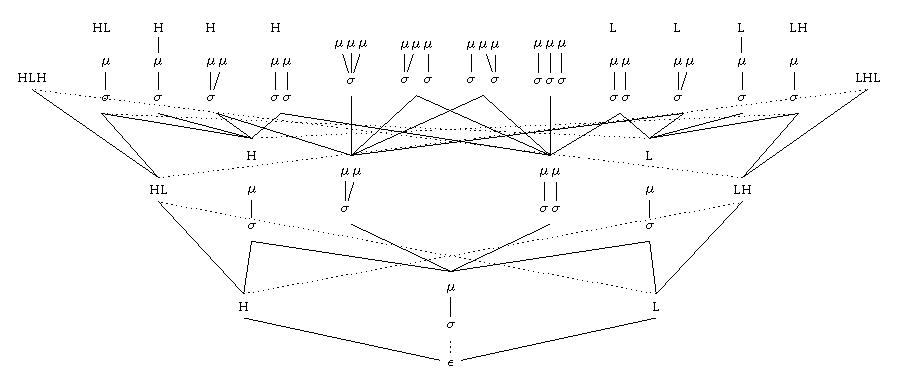
\includegraphics[scale=0.8]{figures/fig.space.pdf}
	\caption{A partially-ordered hypothesis space over ARs}
	\label{fig.AR.space}
\end{figure}

\subsubsection{Interim Summary}
\label{sec:bufiaar.summary}

To summarise, this subsection has presented a concrete method for
computing the next superfactors of a given AR. Four Expansion Rules
were defined: they expand the structure either by adding a unit on a
single tier or by introducing a new association.

We used adjacency matrices to represent the internal associations, and
stipulated some rules to reduce redundancy. Specific matrix patterns
were shown to diagnose ill-formed structures. For example,
Figure~\ref{fig.bad} illustrates three invalid ARs. An
anti-diagonal (from upper right to lower left) of 1s marks a
line-crossing violation, as in Figure~\ref{bad.assoc1}. A column or
row that is filled exclusively with zero indicates an unassociated tone or mora. Such zero-domination is
problematic when it occurs between two columns or rows that contain
associations, as this pattern indicates that an intervening unit has
been skipped, resulting in an improper association formed across it
(as in \ref{bad.assoc2} and \ref{bad.assoc3}) as they violate the
WFC 1 and 2.

\begin{figure}
	\centering	
	\setlength{\tabcolsep}{5pt}
	\begin{minipage}[t]{0.32\textwidth}
		\centering
		\begin{tikzpicture}[scale=0.8]
			\node (t1) at (2,1) {L};
			\node (t2) at (3,1) {H};
			\node[anchor=base] (c1) at (1,0) {$\mu_1$};
			\node[anchor=base] (c2) at (2,0) {$\mu_2$};
			\node[anchor=base] (c3) at (3,0) {$\mu_3$};
			\node[anchor=base] (c4) at (4,0) {$\mu_4$};
			\node (s1) at (2,-1) {$\sigma_1$};
			\node (s2) at (3,-1) {$\sigma_2$};
			\draw (t1) -- (c1) -- (s1);
			\draw (t1) -- (c2) -- (s1);
			\draw (s2) -- (c4);
			\draw (s2) -- (c3);
			\draw[dotted, line width=0.4mm] (c1) to (t2);
		\end{tikzpicture}
		
		\vspace{0.8em}
		
		\begin{tabular}{c|cc}
			& L & H \\
			\hline
			$\mu_1$ & 1 & \cellcolor{gray!30} 1 \\
			$\mu_2$ &\cellcolor{gray!30} 1& 0 \\
			$\mu_3$ & 0 & 0 \\
			$\mu_4$ & 0 & 0 \\
		\end{tabular}
		\subcaption{lines crossing}
		\label{bad.assoc1}
	\end{minipage}
	\hfill
	\begin{minipage}[t]{0.32\textwidth}
		\centering
		\begin{tikzpicture}[scale=0.8]
			\node (t1) at (2,1) {L};
			\node (t2) at (3,1) {H};
			\node[anchor=base] (c1) at (1,0) {$\mu_1$};
			\node[anchor=base] (c2) at (2,0) {$\mu_2$};
			\node[anchor=base] (c3) at (3,0) {\colorbox{gray!30}{$\mu_3$}};
			\node[anchor=base] (c4) at (4,0) {$\mu_4$};
			\node (s1) at (2,-1) {$\sigma_1$};
			\node (s2) at (3,-1) {$\sigma_2$};
			\draw (t1) -- (c1) -- (s1);
			\draw (t1) -- (c2) -- (s1);
			\draw (s2) -- (c4);
			\draw (s2) -- (c3);
			\draw[dotted, line width=0.4mm] (c4) to (t2);
		\end{tikzpicture}

		\vspace{0.8em}
		
		\begin{tabular}{c|cc}
			& L & H \\
			\hline
			$\mu_1$ & 1 & 0 \\
			$\mu_2$ & 1 & 0 \\
			\rowcolor{gray!30} $\mu_3$ & 0 & 0 \\
			$\mu_4$ & 0 & 1 \\
		\end{tabular}
		\subcaption{mora skipping}
		\label{bad.assoc2}
	\end{minipage}
	\hfill
	% --- Third subtable ---
	\begin{minipage}[t]{0.32\textwidth}
		\centering
		\begin{tikzpicture}[scale=0.8]
			\node (t1) at (2,1) {L};
			\node (t2) at (3,1) {\colorbox{gray!30}{H}};
			\node (t3) at (4,1) {L};
			\node[anchor=base] (c1) at (1,0) {$\mu_1$};
			\node[anchor=base] (c2) at (2,0) {$\mu_2$};
			\node[anchor=base] (c3) at (3,0) {$\mu_3$};
			\node[anchor=base] (c4) at (4,0) {$\mu_4$};
			\node (s1) at (2,-1) {$\sigma_1$};
			\node (s2) at (3,-1) {$\sigma_2$};
			\draw (t1) -- (c1) -- (s1);
			\draw (t1) -- (c2) -- (s1);
			\draw (s2) -- (c4);
			\draw (s2) -- (c3);
			\draw[dotted, line width=0.4mm] (c3) to (t3);
		\end{tikzpicture}
		
		\vspace{0.8em}
		
		\begin{tabular}{c|ccc}
			& L & 	\cellcolor{gray!30}H & L \\
			\hline
			$\mu_1$ & 1 & 	\cellcolor{gray!30}0 & 0 \\
			$\mu_2$ & 1 & 	\cellcolor{gray!30}0 & 0 \\
			$\mu_3$ & 0 & 	\cellcolor{gray!30}0 & 1 \\
			$\mu_4$ & 0 & 	\cellcolor{gray!30}0 & 0 \\
		\end{tabular}
		\subcaption{tone skipping}
		\label{bad.assoc3}
	\end{minipage}
	\caption{Invalid association lines}
	\label{fig.bad}
\end{figure}


An alternative interpretation of skipped units is that they are
\textit{floating}. We distinguish between \textit{floating} and
\textit{unassociated} units. Floating tones, which are common in African
languages, are not associated to any TBU and manifest themselves 
under specific phonological conditions. Unassociated units, by
contrast, are available to be linked during the expansion process.

BUFIA-AR does not express floating tones \textit{per se}, only unassociated
units. In principle, floating tones could be incorporated by either
introducing them into structures explicitly, or by interpreting
unassociated units as floating. We leave this matter for future research.

It should be emphasised that explicitly defining how ARs are expanded
is crucial for two reasons. First, the expansion procedure forms the
basis of BUFIA-AR: without it, the space of possible constraints cannot
be traversed, or even represented, and thus the learnability of AR
constraints cannot be properly understood.  Second, this procedure
highlights the multilinear structure and associations between
autosegmental tiers, which are hallmarks of tonal phonology. 


\subsection{Containment Relation}\label{sec:bufiaar.arcontain}

Section~\ref{sec:bufiaar.nextar} introduces the four ways to obtain next 
superfactors of an AR. This section addresses a different question: 
given two ARs, how can we determine if one AR \textit{contains} the other? 



There is more than one method to achieve this algorithmically.
We use a matrix-based containment checker to determine whether two 
ARs, even with the same tone sequence and the same number of syllable 
and mora, will have the same associations.

The matrix containment follows exactly parallel to the general notion
of any structural containment: matrix $A$ is \textit{contained} in
matrix $B$ if there exists a \textit{submatrix} of $B$, denoted $B'$,
that functions as a restriction discussed in Definition~\ref{def.res}, such that all
relations within $A$ are relatively preserved in correspondence with
those in $B'$, as in Definition~\ref{def.contain}.
The following two definitions (Definition~\ref{def.submatrix} and 
\ref{def.ar.matching}) specialize these concepts to the matrix 
representation of ARs.

\begin{definition}
	\label{def.submatrix}
	\textit{Let matrix $A$ be an $m \times n$ matrix.  Matrix $B$ is a
		\emph{submatrix}
		of $A$ by taking $k \ (1 \leq k \leq m)$ contiguous rows and $v \ (1 \leq v
		\leq n)$ contiguous columns from $A$.}\footnote{The term ``submatrix" is
		generally defined by deleting arbitrary rows and/or columns from the original
		matrix. However, in our case, we require a more restricted definition: the
		remaining rows and columns must be \textit{contiguous} in the original matrix,
		which reflects tonal locality.}
\end{definition}

\begin{definition}
	\label{def.ar.matching}
	\textit{
		An $m\times n$ matrix $A = [a_{ij}]$ is \emph{contained} in a matrix $B (A
		\sqsubseteq B)$, if there exists an $m\times n$ submatrix in B, denoted by $B' =
		[b'_{ij}]$ such that for all $i \in [0,m] ,j \in [0,n],\ b'_{ij}  \geq \ a_{ij}
		$.}
\end{definition}

Definition \ref{def.submatrix} defines what a submatrix is.  Definition
\ref{def.ar.matching}
states that a smaller matrix \( A = [a_{ij}] \) is contained in a larger matrix
\( B =
[b_{ij}] \) if we can find a submatrix \( B' \subseteq B \), with the same
dimensions as \( A \), such that the value of each entry in \( B' \) 
is at least as large as the corresponding entry in \( A \); that is, \(
b'_{ij} \geq a_{ij} \) for all \( i, j \). Since the entries of these matrices
are binary, this condition implies two cases:

\begin{enumerate}[label=(\alph*)]
	\item If \( a_{ij} = 1 \), meaning there is an association between node \(
	i \) and node \( j \) in the smaller matrix \( A \), then \( b'_{ij} \) must
	also be 1. This ensures an association found in \( A \) is preserved in \(B'\)
	at the same position;
	\item If \( a_{ij} = 0 \), meaning no association exists between node \( i \)
	and node \( j \) in the smaller matrix \( A \), then \( b'_{ij} \) may be
	either 0 or 1. In other words, \( B' \) may or may not have an
	association at the corresponding position. It is permitted to contain
	additional associations beyond those in \( A \), but it must not omit any that
	are present in \( A \).
\end{enumerate}

The comparison proceeds by first identifying whether the tonal string of one
structure is contained within another, and then verifying whether the
corresponding association matrices align. Even when a tonal substring match
is found, containment is established only if the associated tone--mora and
mora--syllable submatrices match within the aligned region. The full algorithm
is provided in the Supplementary Material, along with a detailed walk-through.
Figure~\ref{fig:matrixmatching} illustrates this procedure:
(\subref{fig:matrix-light}) is not contained in
(\subref{fig:matrix-heavy}) or (\subref{fig:matrix-super}),
whereas (\subref{fig:matrix-heavy}) is contained in
(\subref{fig:matrix-super}), since the submatrices in
(\subref{fig:matrix-super}) (the shaded cells) match the matrices of
(\subref{fig:matrix-heavy}) in terms of associations
as well as tonal strings, but do not match those of
(\subref{fig:matrix-light}).
\begin{figure}[ht]
\centering 
\setlength{\tabcolsep}{5pt}
% --- Block (a) ---
	\begin{subtable}[t]{0.25\textwidth}
		\centering
		\begin{tikzpicture}[scale = 0.9]
			\node (bt1) at (1,1) {L};
			\node (bt2) at (2,1) {H};
			\node (bc1) at (1.5,0) {$\mu_1$};
			\node (bs1) at (1.5,-1) {$\sigma_1$};
			\draw (bt1) -- (bc1) -- (bs1);
			\draw (bt2) -- (bc1) -- (bs1);
			
			% Array 1 (b)
			\node (barray1) at (1.5,-2.5) {
			  \begin{tabular}{c|cc}
			    & L & H \\
			    \hline
			    $\mu_1$ & 1 & 1
			  \end{tabular}
			};
			
			% Array 2 (b)
			\node (barray2) at (1.5, -4.2) {
				\begin{tabular}{c|c}
					& $\mu_1$ \\
					\hline
					$\sigma_1$ & 1  
				\end{tabular}
				};
		\end{tikzpicture}
		\subcaption{}
		\label{fig:matrix-light}
	\end{subtable}
	\hfill
	% --- Block (B) ---
	\begin{subtable}[t]{0.25\textwidth}
		\centering
		\begin{tikzpicture}[scale = 0.9]
			\node (ct1) at (1,1) {L};
			\node (ct2) at (2,1) {H};
			\node (cc1) at (1,0) {$\mu_1$};
			\node (cc2) at (2,0) {$\mu_2$};
			\node (cs1) at (1.5,-1) {$\sigma_2$};
			\draw (ct1) -- (cc1) -- (cs1);
			\draw (ct2) -- (cc2) -- (cs1);
			
			% Array 1
			\node (carray1) at (1.5, -2.5) {
				\begin{tabular}{c|cc}
					& L & H \\
					\hline
					$\mu_1$ & 1 & 0 \\
					$\mu_2$ & 0 & 1 
				\end{tabular}
				};
			
			% Array 2 
			\node (carray2) at (1.5, -4.2) {				
			\begin{tabular}{c|cc}
					& $\mu_1$ & $\mu_2$ \\
					\hline
					$\sigma_1$ & 1  & 1
				\end{tabular}};
		\end{tikzpicture}
		\subcaption{}
		\label{fig:matrix-heavy}
	\end{subtable}
	\hfill
	% --- Block (C) ---
	\begin{subtable}[t]{0.3\textwidth}
		\centering
		\begin{tikzpicture}[scale = 0.9]
			\node (dt0) at (0,1) {H};
			\node (dt1) at (1,1) {L};
			\node (dt2) at (2,1) {H};
			\node (dc0) at (0,0) {$\mu_1$};
			\node (dc1) at (1,0) {$\mu_2$};
			\node (dc2) at (2,0) {$\mu_3$};
			\node (ds0) at (0,-1) {$\sigma_1$};
			\node (ds1) at (1.5,-1) {$\sigma_2$};
			\draw (dt1) -- (dc1) -- (ds1);
			\draw (dt0) -- (dc0) -- (ds0);
			\draw (dt2) -- (dc2) -- (ds1);
			\draw (dt1) -- (dc0);
			
			% Array 1 (c)
			\node (darray1) at (1, -2.5) {
				\begin{tabular}{c|c>{\columncolor[gray]{0.9}}c>{\columncolor[gray]{0.9}}c}
					& H & L & H \\
					\hline
				$\mu_1$ & 1	&	1 & 0 \\
				$\mu_2$ & 0 & \cellcolor{gray!50}1 & \cellcolor{gray!50}0\\
				$\mu_3$ &0 &\cellcolor{gray!50}0&\cellcolor{gray!50}1\\
				\end{tabular}
				};
			
			% Array 2 (c)
			\node (darray2) at (1, -4.5) {
					\begin{tabular}
						{c|c>{\columncolor[gray]{0.9}}c>{\columncolor[gray]{0.9}}c}
					& $\mu_1$ & $\mu_2$ & $\mu_3$\\
					\hline
					$\sigma_1$ & 1 & 0 & 0\\
					$\sigma_2$ & 0 &  \cellcolor{gray!50} 1 & \cellcolor{gray!50} 1\\
				\end{tabular}
				};
		\end{tikzpicture}
		\subcaption{}
		\label{fig:matrix-super}
	\end{subtable}
	\hfill
	\caption{Light LH (11a), heavy LH (11b), 
	and a superfactor of heavy LH (11c)}
	\label{fig:matrixmatching}
\end{figure}


\subsection{Summary}
This section established BUFIA-AR, which and implementation 
of two functions that are core to the BUFIA-AR framework: 
\textsc{NextSupFact} and \textsc{Contain}, which are 
used in the case study described in the next section.


\section{Case Study: Hausa} \label{sec:hausa} is grounded in autosegmental 
theory. In particular, we explained the rationale

This section presents a case study applying BUFIA-AR to identify
tonotactic constraints over ARs in Hausa. We examine Hausa because
suitable data was available; we are unaware of a similar dataset for
Mende. The analysis focuses on non-derived native Hausa words,
examples of which are shown in Table~\ref{ex.hausa.words}. As mentioned
earlier, in Hausa monomoraic syllables can bear either H or L, but
cannot bear contours. A bimoraic syllable can take an HL contour (each
tone associates to one mora) but LH contours are not allowed. Lastly,
Hausa does not have superheavy syllables, therefore monosyllabic
three-tone contours are also not allowed.  


\begin{table}[h!]
	\centering
	\renewcommand{\arraystretch}{2}
	\begin{tabular}{lllll}
		\hline
		
		\textbf{Monosyllabic} 
		& \makecell{\textipa{\texthtd}áa \\ `son’} 
		& \makecell{mèe \\ `what’} 
		& \makecell{mâi \\ `oil’} 
		
		&  \\ \hline
		\textbf{Disyllabic} 
		& \makecell{\textipa{\texthtk}á.sáa \\ `land’} 
		& \makecell{mù.tûm \\ `person’} 
		& \makecell{tú.dùu \\ `hill’} 
		& \makecell{màa.gée \\ `cat’}  \\
		\hline
		
		\textbf{Trisyllabic} 
		& \makecell{í.nú.wàa \\ `shadow’} 
		& \makecell{\textipa{\texthtk}àn.\textipa{\texthtk}á.ráa \\ `ice/snow’} 
		& \makecell{múu.jì.yáa \\ `owl'} 
		& \makecell{fà.dá.màa\\ `swamp'} \\ \hline
	\end{tabular}
	\caption{Nonderived native Hausa words \citep{wold-4}}
	\label{ex.hausa.words}
\end{table}

\citet[p.606]{Newmanbook} notes
non-derived disyllabic words exhibit canonical normal tone
patterns: H.L, L.H, and H.H. For trisyllabic nouns, H.L.H,
H.H.L, L.H.L, and L.H.H are very common, but L.L.H is less
common with basic lexical items. Words ending in L.L, either 
disyllabic or polysyllabic words containing L.L, are relatively uncommon, 
especially when the second syllable bears a long vowel. 
When L.L forms do occur, they are typically restricted to 
ideophones or loanwords \citep[p.606]{Newmanbook}. 
\citet{zoll2003optimal} argues that the absence of H.L.L
and L.L.H is a result of the constraint \textsc{*Lapse} (which
forbids L from spreading across adjacent syllables) outranking
\textsc{*Clash} (which forbids H from spreading across two syllables).
In addition, for canonical, non-derived forms falling (F) tones 
typically fall on the last syllable \citep[p.606]{Newmanbook}.

Based on the above, the linguistically attested constraints in Hausa 
are summarised in Table~\ref{rules}, which are translated into 
AR constraints in Table~\ref{tab.rule.constraints}. In this 
study, we treat these constraints as the baseline grammar against which 
performance of BUFIA models is evaluated. Specifically, we investigate 
whether BUFIA-AR can accurately learn AR-based constraints, and 
if so, how the computationally attested constraints (henceforth, 
BUFIA constraints) correspond to previously identified linguistic 
ones (baseline constraints). We also include a BUFIA-string model 
as a comparison, which learns constraints over the same 
data using string representations.

\begin{table}
	\centering
	\begin{tabular}{ll}
		\toprule
		\textbf{Generalisations} & \textbf{Interpretation}                              \\
		\midrule
		\textbf{\textsc{*Rise$_\sigma$}}     & Syllables may not be associated with rising tones (LH) \\
		\textbf{\textsc{*Contour$_{\mu}$}}   & Moras may be associated with at most one tone.      \\
		\textbf{\textsc{*3t-Contour}}        & No trimoraic contour  \\
		\textbf{\textsc{*NonFinal-Fall}}     & No nonfinal HL contour for polysyllabic words         \\
		\textbf{\textsc{*Lapse}}             & No L spreading across syllables \\
		\bottomrule
	\end{tabular}
	\caption{Phonological Generalisations in Hausa}
	\label{rules}
\end{table}
\begin{table}
	\centering
	\begin{tabular}{ccccc}
		\toprule
		\textbf{\textsc{*Rise$_\sigma$}} &
		\textbf{\textsc{*Contour$_{\mu}$}} &
		\textbf{\textsc{*3t-Contour}} &  
		\textbf{\textsc{*NonFinal-Fall}} &
		\textbf{\textsc{*Lapse}} \\
		\midrule
		\begin{tikzpicture}
			\node (bt1) at (-.4,0.8) {L};
			\node (bt2) at (.4,0.8) {H};
			\node (bc1) at (-.4,0) {$\mu$};
			\node (bc2) at (0.4,0) {$\mu$};
			\node (bs1) at (0,-0.8) {$\sigma$};
			\draw (bt1) -- (bc1) -- (bs1);
			\draw (bt2) -- (bc2) -- (bs1);
		\end{tikzpicture} &
		\begin{tikzpicture}
			\node (bt1) at (-.4,0.8) {X};
			\node (bt2) at (.4,0.8) {X};
			\node (bc1) at (0,0) {$\mu$};
			\node (bs1) at (0,-0.8) {$\sigma$};
			\draw (bt1) -- (bc1) -- (bs1);
			\draw (bt2) -- (bc1) -- (bs1);
		\end{tikzpicture} &
		\begin{tikzpicture}
			\node (bt1) at (-.4,0.8) {$\mu$};
			\node (bt2) at (.0,0.8) {$\mu$};
			\node (bt3) at (.4,0.8) {$\mu$};
			\node (bs1) at (0,-0) {$\sigma$};
			\draw (bt1)  -- (bs1);
			\draw (bt2) -- (bs1);
			\draw (bt3) -- (bs1);
		\end{tikzpicture} &
		\begin{tikzpicture}
			\node (bt1) at (-.6,0.8) {H};
			\node (bt2) at (0,0.8) {L};
			\node (bc1) at (-.6,0) {$\mu$};
			\node (bc2) at (0,0) {$\mu$};
			\node (bs1) at (-.3,-0.8) {$\sigma$};
			\node (bc3) at (0.6,0) {$\mu$};
			\node (bs2) at (0.6,-0.8) {$\sigma$};
			\draw (bt1) -- (bc1) -- (bs1);
			\draw (bt2) -- (bc2) -- (bs1);
			\draw (bc3) -- (bs2);    
		\end{tikzpicture} &
		\begin{tikzpicture}
			\node (bt1) at (0,0.8) {L};
			\node (bc1) at (-.4,0) {$\mu$};
			\node (bc2) at (.4,0) {$\mu$};
			\node (bs1) at (-.4,-0.8) {$\sigma$};
			\node (bs2) at (.4,-0.8) {$\sigma$};
			\draw (bt1) -- (bc1) -- (bs1);
			\draw (bt1) -- (bc2) -- (bs2);
		\end{tikzpicture} \\
		\bottomrule
	\end{tabular}
	\caption{Phonological Generalisations Translated into forbidden ARs}
	\label{tab.rule.constraints}
\end{table}




\subsection{Experiment Setup}
The data used for the current experiment comes from the Hausa dataset
\citep{wold-4} in The World Loanword Database (WOLD) \citep{wold}. It
consists of around 1460 core words whose meanings are present in the
Loanword Typology meaning list. This list includes forms and concepts
that all languages have terms for. For the Hausa dataset, the
vocabulary contains 1668 core meaning-word pairs, along with other
information in fields titled Form, Meaning, Loanword Status, and
Analysability. To ensure consistency with previous generalisations, 
which are based on canonical, non-derived tonal patterns,
we restrict our dataset to monomorphemic words that are clearly 
non-borrowed, and all others were filtered out. In addition, forms 
containing glides (\textipa{\texthtk}w, \textipa{\texthtk}y, kw, ky, gw, gy) 
were excluded to avoid 
ambiguous syllabification and uncertain syllable weight.
As a result, a total of 621 words transcribed in orthography
remained and were stored in a .csv file.
All orthographic forms were first syllabified \citep{kodner2016} then
converted into its corresponding AR representation using the method
described in \citet{jardine2015concatenation}. 
Table~\ref{tab.conversion} shows how an orthographic form with
tonal markers is transformed into its corresponding matrix
representation. After conversion and removal of duplicate ARs, 64
distinct AR types were identified among the 621 words, which serve as
the positive dataset on which BUFIA-AR operates.
\begin{table}[ht]
	\centering
	\begin{tabular}{
			>{\centering\arraybackslash}m{1.2cm}|
			>{\centering\arraybackslash}m{1cm}|
			>{\centering\arraybackslash}m{3.2cm}|
			>{\centering\arraybackslash}m{8cm}
		}
		\toprule
		\textbf{Form} &
		\textbf{Tones} &
		\textbf{AR Diagram} &
		\textbf{Matrix-based Encodings} \\
		\midrule
		\makecell{\textit{k\`oo.g\'ii}\\`river'}
		&
		LH
		&
		\begin{tikzpicture}[scale=.85,every node/.style={scale=.85}]
			\node (t1) at (2,1) {L};
			\node (t2) at (3,1) {H};
			
			\node (c1) at (1,0) {$\mu_1$};
			\node (c2) at (2,0) {$\mu_2$};
			\node (c3) at (3,0) {$\mu_3$};
			\node (c4) at (4,0) {$\mu_4$};
			
			\node (s1) at (2,-1) {$\sigma_1$};
			\node (s2) at (3,-1) {$\sigma_2$};
			
			\draw (t1)--(c1)--(s1);
			\draw (t1)--(c2)--(s1);
			\draw (t2)--(c3)--(s2);
			\draw (t2)--(c4)--(s2);
		\end{tikzpicture}
		&
		\[
		\begin{array}{c|cc}			
		& \text{ L } & \text{ H }\\
			\hline
			\mu_1 & 1 & 0\\
			\mu_2 & 1 & 0\\
			\mu_3 & 0 & 1\\
			\mu_4 & 0 & 1
		\end{array}
		\quad
		\begin{array}{c|cccc}
			& \,\mu_1\, &\,\mu_2 \,& \,\mu_3\, &\, \mu_4\,\\
			\hline
			\sigma_1 & 1 & 1 & 0 & 0\\
			\sigma_2 & 0 & 0 & 1 & 1
		\end{array}
		\]
		\\
		\midrule		
		\makecell{\textit{mù.tûm}\\`person'}
		&
		LF
		&
		\begin{tikzpicture}[scale=.85,every node/.style={scale=.85}]
			\node (t0) at (1,1) {L};
			\node (t1) at (2,1) {H};
			\node (t2) at (3,1) {L};
			
			\node (c1) at (1,0) {$\mu_1$};
			\node (c2) at (2,0) {$\mu_2$};
			\node (c3) at (3,0) {$\mu_3$};
			
			\node (s1) at (1,-1) {$\sigma_1$};
			\node (s2) at (2.5,-1) {$\sigma_2$};
			
			\draw (t0)--(c1)--(s1);
			\draw (t1)--(c2)--(s2);
			\draw (t2)--(c3)--(s2);
		\end{tikzpicture}
		&
		\[
		\begin{array}{c|ccc}
			& \text{ L } & \text{ H } & \text{ L }\\
			\hline
			\mu_1 & 1 & 0 & 0\\
			\mu_2 & 0 & 1 & 0\\
			\mu_3 & 0 & 0 & 1
		\end{array}
		\quad
		\begin{array}{c|ccc}
			& \,\mu_1\, &\,\mu_2 \,& \,\mu_3\,\\
			\hline
			\sigma_1 & 1 & 0 & 0\\
			\sigma_2 & 0 & 1 & 1
		\end{array}
		\]
		\\		\bottomrule
	\end{tabular}
	
	\caption{Corresponding lexical forms, ARs, and their matrix-based encodings.}
	\label{tab.conversion}
\end{table}

We ran BUFIA-AR with the number of syllables,
moras, and tones limited to a maximum of three. 
The number three was chosen for two reasons. 
First, two of the baseline constraints in
Table~\ref{tab.rule.constraints} have three moras. 
If BUFIA-AR stopped searching for constraints before 
structures with three moras, it would not find those 
constraints. Second, we wanted to show that BUFIA-AR 
could return constraints with unassociated units, which 
is a unique aspect of ARs as compared to linear 
representations.

\subsection{Evaluation}
In this section, we provide two types of evaluation: qualitative and 
quantitative. The qualitative evaluation examines how the grammar learned 
by BUFIA-AR compares with the baseline grammar. The quantitative 
evaluation uses $k$-fold cross-validation,
a common method in machine learning for assessing 
how well a predictive model generalises to unseen data. 
\subsubsection{Qualitative Evaluation: Constraints Comparison}
BUFIA-AR found 11 constraints when the numbers of 
syllable, mora, and tone are limited to three. 
More generally, the output of BUFIA-AR for smaller 
values $s,\mu$ and the number of tones are subsets 
of the 11 constraints in Table~\ref{tab.results}. 
Cells with a dash indicate that no constraints were 
found with those $s$ and $\mu$ sizes.  

\begin{table}[hbt]
	\centering
	\begin{tabular}{c|c|c|c}
		\toprule
		& $\mu = 1$ & $\mu = 2$ & $\mu = 3$ \\
		\midrule
		$s = 1$ & 
		\begin{subtable}[t]{1.2cm}
			\begin{tikzpicture}[scale=.85,every node/.style={scale=.85}]
				\node (bt1) at (-.4,0.8) {L};
				\node (bt2) at (.4,0.8) {H};
				\node (bc1) at (0,0) {$\mu$};
				\node (bs1) at (0,-0.8) {$\sigma$};
				\draw (bt1) -- (bc1) -- (bs1);
				\draw (bt2) -- (bc1);
			\end{tikzpicture}
				\subcaption{}\label{cons.a}
			\end{subtable}
		\begin{subtable}[t]{1.2cm}
				\centering
			\begin{tikzpicture}[scale=.85,every node/.style={scale=.85}]
				\node (bt1) at (-.4,0.8) {H};
				\node (bt2) at (.4,0.8) {L};
				\node (bc1) at (0,0) {$\mu$};
				\node (bs1) at (0,-0.8) {$\sigma$};
				\draw (bt1) -- (bc1) -- (bs1);					
				\draw (bt2) -- (bc1);
			\end{tikzpicture}
				\subcaption{}
				\label{cons.b}
		\end{subtable}
			&
		\begin{subtable}[t]{1.2cm}
			\begin{tikzpicture}[scale=.85,every node/.style={scale=.85}]
				\node (bt1) at (-.4,0.8) {L};
				\node (bt2) at (.4,0.8) {H};
				\node (bc1) at (-.4,0) {$\mu$};
				\node (bc2) at (.4,0) {$\mu$};
				\node (bs1) at (0,-0.8) {$\sigma$};
				\draw (bt1) -- (bc1) -- (bs1);
				\draw (bt2) -- (bc2) -- (bs1);
			\end{tikzpicture}
			\subcaption{}
			\label{cons.c}
		\end{subtable}
			&
		\begin{subtable}[t]{1.2cm}
		\begin{tikzpicture}[scale=.85,every node/.style={scale=.85}]
				\node (bc1) at (-.4,0) {$\mu$};
				\node (bc2) at (.4,0) {$\mu$};
				\node (bc3) at (0,0) {$\mu$};
				\node (bs1) at (0,-0.8) {$\sigma$};
				\draw (bc1) -- (bs1);
				\draw (bc2) -- (bs1);
				\draw (bc3) -- (bs1);
			\end{tikzpicture}
			\subcaption{}
			\label{cons.d} 
		\end{subtable}\\
		\midrule
		$s = 2$ & - & - &
		\begin{subtable}[t]{1.2cm}
			\begin{tikzpicture}[scale=.85,every node/.style={scale=.85}]
				\node (bt1) at (-.4,0.8) {H};
				\node (bt2) at (.4,0.8) {L};					
				\node (bc1) at (-.4,0) {$\mu$};
				\node (bc2) at (0,0) {$\mu$};
				\node (bc3) at (.4,0) {$\mu$};
				\node (bs1) at (-.4,-0.8) {$\sigma$};
				\node (bs2) at (.4,-0.8) {$\sigma$};
				\draw (bt1) -- (bc1) -- (bs1);
				\draw (bt2) -- (bc2) -- (bs1);
				\draw (bt2) -- (bc3) -- (bs2);
			\end{tikzpicture}\subcaption{}\label{cons.e}
		\end{subtable} \hfill
		\begin{subtable}[t]{1.2cm}
			\begin{tikzpicture}[scale=.85,every node/.style={scale=.85}]
					\node (bt1) at (-.4,0.8) {H};
					\node (bt2) at (.4,0.8) {L};
					\node (bc1) at (-.4,0) {$\mu$};
					\node (bc2) at (0,0) {$\mu$};
					\node (bc3) at (.4,0) {$\mu$};
					\node (bs1) at (-.4,-0.8) {$\sigma$};
					\node (bs2) at (.4,-0.8) {$\sigma$};
					\draw (bt1) -- (bc1) -- (bs1);
					\draw (bt1) -- (bc2) -- (bs2);
					\draw (bt2) -- (bc3) -- (bs2);
				\end{tikzpicture}
				\subcaption{}
				\label{cons.f}
		\end{subtable} \hfill
		\begin{subtable}[t]{1.2cm}
			\begin{tikzpicture}[scale=.85,every node/.style={scale=.85}]
					\node (bt1) at (0,0.8) {H};
					\node (bt2) at (.4,0.8) {L};
					\node (bt3) at (.8,0.8) {H};
					\node (bc1) at (-.4,0) {$\mu$};
					\node (bc2) at (0,0) {$\mu$};
					\node (bc3) at (.4,0) {$\mu$};
					\node (bs1) at (-.4,-0.8) {$\sigma$};
					\node (bs2) at (.4,-0.8) {$\sigma$};
					\draw (bt1) -- (bc1) -- (bs1);
					\draw (bt1) -- (bc2) -- (bs1);
					\draw (bt1) -- (bc3) -- (bs2);
			\end{tikzpicture}\subcaption{}\label{cons.g}
		\end{subtable}
		\\ \midrule
		$s = 3$ & - & - &
		\begin{subtable}[t]{1.2cm}
			\begin{tikzpicture}[scale=.85,every node/.style={scale=.85}]
				\node (bt1) at (-.4,0.8) {H};
				\node (bt2) at (.4,0.8) {L};
				\node (bc1) at (-.4,0) {$\mu$};
				\node (bc2) at (0,0) {$\mu$};
				\node (bc3) at (.4,0) {$\mu$};
				\node (bs1) at (-.4,-0.8) {$\sigma$};
				\node (bs2) at (0,-0.8) {$\sigma$};
				\node (bs3) at (.4,-0.8) {$\sigma$};
				\draw (bt1) -- (bc1) -- (bs1);
				\draw (bt2) -- (bc2) -- (bs2);					
				\draw (bt2) -- (bc3) -- (bs3);
			\end{tikzpicture}\subcaption{}\label{cons.h}
		\end{subtable}			\hfill
		\begin{subtable}[t]{1.2cm}
			\begin{tikzpicture}[scale=.85,every node/.style={scale=.85}]
				\node (bt1) at (-.4,0.8) {L};
				\node (bt2) at (0,0.8) {H};
				\node (bt3) at (.4,0.8) {L};
				\node (bc1) at (-.4,0) {$\mu$};
				\node (bc2) at (0,0) {$\mu$};					
				\node (bc3) at (.4,0) {$\mu$};
				\node (bs1) at (-.4,-0.8) {$\sigma$};
				\node (bs2) at (0,-0.8) {$\sigma$};
				\node (bs3) at (.4,-0.8) {$\sigma$};
				\draw (bt1) -- (bc1);
				\draw (bt1) -- (bc2);					
				\draw (bt1) -- (bc3);
				\draw (bc1) -- (bs1);
				\draw (bc2) -- (bs2);
				\draw (bc3) -- (bs3);
			\end{tikzpicture}\subcaption{}\label{cons.i}
		\end{subtable}  \hfill
		\begin{subtable}[t]{1.2cm}
			\begin{tikzpicture}[scale=.85,every node/.style={scale=.85}]
				\node (bt1) at (-.4,0.8) {H};
				\node (bt2) at (0,0.8) {L};
				\node (bt3) at (.4,0.8) {H};					
				\node (bc1) at (-.4,0) {$\mu$};
				\node (bc2) at (0,0) {$\mu$};
				\node (bc3) at (.4,0) {$\mu$};
				\node (bs1) at (-.4,-0.8) {$\sigma$};
				\node (bs2) at (0,-0.8) {$\sigma$};					
				\node (bs3) at (.4,-0.8) {$\sigma$};
				\draw (bt1) -- (bc1);
					\draw (bt1) -- (bc2);
				\draw (bc1) -- (bs1);
				\draw (bc2) -- (bs2);
				\draw (bc3) -- (bs3);
			\end{tikzpicture}\subcaption{}\label{cons.j}
		\end{subtable}  \hfill
		\begin{subtable}[t]{1.2cm}
			\begin{tikzpicture}[scale=.85,every node/.style={scale=.85}]
					\node (bt1) at (-.4,0.8) {L};
					\node (bt2) at (0,0.8) {H};
					\node (bt3) at (.4,0.8) {L};
					\node (bc1) at (-.4,0) {$\mu$};
					\node (bc2) at (0,0) {$\mu$};
					\node (bc3) at (.4,0) {$\mu$};
					\node (bs1) at (-.4,-0.8) {$\sigma$};
					\node (bs2) at (0,-0.8) {$\sigma$};
					\node (bs3) at (.4,-0.8) {$\sigma$};
					\draw (bt1) -- (bc1);
					\draw (bt2) -- (bc2);
					\draw (bt2) -- (bc3);
					\draw (bc1) -- (bs1);
					\draw (bc2) -- (bs2);
					\draw (bc3) -- (bs3);
				\end{tikzpicture}
				\subcaption{}
				\label{cons.k}
			\end{subtable}\\
	\bottomrule
	\end{tabular}
	\caption{Hausa constraints returned by BUFIA-AR  when $s \leq 3, \   t \leq 3, \ \mu \leq 3$}
	\label{tab.results}
\end{table}



As shown in Table~\ref{sec5.tab.compare}, all of these
constraints together constitute three categories: one where the
baseline constraints have matching BUFIA constraints, one where the
baseline constraints do not have corresponding BUFIA constraints, and
one where BUFIA constraints do not have corresponding baseline
constraints. In Table~\ref{sec5.tab.compare}, this third category of
constraints also provides names for the BUFIA constraints
(\ref{cons.e}-\ref{cons.h}) in terms of the melody and syllabification
implicated by the structures in Figure~\ref{tab.results}. Boldface 
indicates the tone on heavy syllables. These labels serve only 
as shorthand for the ARs shown in Table~\ref{sec5.tab.compare} and 
may be ambiguous, as they do not fully capture the structures. 

\begin{table}[h!]
	\centering
	\begin{tabular}{p{4cm}p{3.5cm}p{3.5cm}}
		\toprule
		\textbf{Present in both \newline BUFIA and Baseline} 
		& \textbf{Baseline Constraints \newline Absent from BUFIA} 
		& \textbf{BUFIA Constraints \newline Absent from Baseline} \\
		\midrule
		\textsc{*Rise}$_\sigma$~(\ref{cons.c})\newline
		\textsc{*Contour}$_\mu$~(\ref{cons.a}--\ref{cons.b})\newline
		\textsc{*3T-Contour}~(\ref{cons.d})\newline
		& \textsc{*NonFinal-Fall}\newline
		\textsc{*Lapse}
		& \textsc{*F.L}~(\ref{cons.e})\newline
		\textsc{*H.F}~(\ref{cons.f})\newline
		\textsc{*\textbf{H}.H-LH}~(\ref{cons.g})\newline
		\textsc{*H.L.L}~(\ref{cons.h})\newline
		\textsc{*L.L.L-HL}~(\ref{cons.i})\newline
		\textsc{*H.H-LH}~(\ref{cons.j})\newline
		\textsc{*L.H.H-L}~(\ref{cons.k})\\
		\bottomrule
	\end{tabular}
	\caption{Comparing baseline constraints with BUFIA constraints}
	\label{sec5.tab.compare}
\end{table}

The first category is when the BUFIA-AR attested constraints align
with the linguistic generalisations previously argued for in the
literature. For monosyllabic forms (when \(s=1\)), BUFIA-AR returned
four constraints: a monomoraic LH (\ref{cons.a}), a monomoraic HL
(\ref{cons.b}), a bimoraic LH (\ref{cons.c}), and a trimoraic
structure (\ref{cons.d}).  Each of these matches a baseline
constraint.  In particular, (\ref{cons.a}) and (\ref{cons.b}) together
account for the absence of monomoraic contour tones, or the constraint
\textsc{*Contour}$_\mu$. The two constraints further rule out any
structures in which a single mora associates with more than two
tones. Secondly, the BUFIA-constraint (\ref{cons.c}) precisely forbids 
a heavy LH contour, which is identical to \textsc{*Rise} constraint in
Table~\ref{tab.rule.constraints}. Its counterpart, a heavy HL
syllable, is not returned, which appropriately addresses the contour
asymmetry problem discussed earlier. Finally, (\ref{cons.d}) correctly
disallows trimoraic syllables as expressed by the constraint
\textsc{*3T-Contour}. BUFIA-AR does not return any specific tonal
forms for this structure, since any tonal sequence it carries will
ultimately violate the forbidden structure.
One thing to note here is that both \textsc{Contour}{$_\mu$} and
\textsc{3T-Contour} describe structural information:
\textsc{Contour}{$_\mu$} prohibits binary branching on a mora node,
while \textsc{3T-Contour} prohibits ternary branching on a syllable
node. The reason that \textsc{3T-Contour} can be ruled out by a single
constraint \ref{cons.d}, whereas two constraints, \ref{cons.a} and
\ref{cons.b}, are needed to account for \textsc{Contour}{$_\mu$} is
that in the current implementation, tonal specifications must be fully
specified, and we did not include an umbrella feature, or permit
under-specified tonal nodes, that would match both H and L.
Overall, BUFIA constraints (\ref{cons.a}-\ref{cons.d}) correctly
reflect frequently reported patterns regarding the tonal inventory,
TBU, and syllable weight, and arguably cover some of the most
fundamental aspects of Hausa tonology. This demonstrates that BUFIA-AR
is not only capable of learning these tonotactic patterns but also
expressing them in terms of ARs.
The second category regards baseline constraints without matching
BUFIA constraints. There are two of these constraints,
\textsc{*NonFinal-Fall} and \textsc{*Lapse}. Each of these appear to
be partially, not totally, accounted for by some of the BUFIA
constraints. For example, constraint~(\ref{cons.e}) partially captures
the generalisation \textsc{*NonFinal-Fall}, which requires that HL
contours do not occur in non-final position, and in particular, when
the following syllable bears a L tone. This is a clue that the BUFIA
constraints appear to allow for the possibility of an HL contour
followed by a H syllable because no constraint banning such a
configuration was returned. Indeed, a reverse search revealed six
words that exhibit these structures, as shown in Example 
(\ref{hlhwords}).\footnote{\citet[p.~607]{Newmanbook} lists eight
	non-derived words with an initial HL tone, possibly reflecting the
	historical loss of a low-tone vowel. The word \textit{kûn.née} `the ear'
	is one of
	these; the others did not appear in Newman’s records.} These
data points indicate that the constraint \textsc{*NonFinal-Fall} is
too strong and it must be further refined if it is to account for the
full range of observed data.
\ex Hausa words exhibiting HL.H pattern (\textsc{*NonFinal-Fall})

\label{hlhwords}
\setlength{\tabcolsep}{0pt} % reduce horizontal padding
\renewcommand{\arraystretch}{1} % single spacing
\begin{tabular}{@{}l@{\hspace{0.8em}}l@{\hspace{1em}}l@{}}
	a. & jîn.\textipa{\texthtk}ái        & ``the pity’’ \\
	b. & kûn.née        & ``the ear’’ \\
	c. & tsûm.máa       & ``the handkerchief or rag’’ \\
	d. & sâi.wáa        & ``the root’’ \\
	e. & bâu.táa        & ``worship’’ \\
	f. & yân.yáa.wàa    & ``the fox (fennec of Sahara)’’ \\
\end{tabular}
\xe


Consider the next baseline constraint \textsc{*Lapse}, which disfavours
the L-tone spreading, therefore predicts the absence of H.L.L and L.L.H 
\citep{zoll2003optimal}. The BUFIA constraint
(\ref{cons.h}) *H.L.L bans one form of H.L.L when all three syllables
are monomoraic, but does not entail banning other H.L.L structures, 
such as ones that contain a heavy syllable. An
example in the data is the word \textit{sá.bòo.dà} `because.' Even
though this word expresses the H.L.L pattern, it does not contain the
structure shown in (\ref{cons.h}) and therefore it satisfies BUFIA
constraint (\ref{cons.h}) *H.L.L.\footnote{Visually, \raisebox{-.4em}{
		\begin{tikzpicture}[scale=1,baseline=(current bounding box.center)]
			\node (bt1) at (-0.4,0.8) {\scriptsize H};
			\node (bt2) at (0.4,0.8) {\scriptsize L};
			\node (bc1) at (-0.4,0) {\scriptsize $\mu_1$};
			\node (bc2) at (0,0) {\scriptsize $\mu_2$};
			\node (bc3) at (0.4,0) {\scriptsize $\mu_3$};
			\node (bs1) at (-0.4,-0.8) {\scriptsize $\sigma_1$};
			\node (bs2) at (0,-0.8) {\scriptsize $\sigma_2$};
			\node (bs3) at (0.4,-0.8) {\scriptsize $\sigma_3$};
			\draw (bt1) -- (bc1) -- (bs1);
			\draw (bt2) -- (bc2) -- (bs2);
			\draw (bt2) -- (bc3) -- (bs3);
		\end{tikzpicture}
	}
	might appear to be contained in
	\raisebox{-.4em}{
		\begin{tikzpicture}[scale=1,baseline=(current bounding box.center)]
			\node (bt1) at (-0.4,0.8) {\scriptsize H};
			\node (bt2) at (0.4,0.8) {\scriptsize L};
			\node (bc1) at (-0.4,0) {\scriptsize $\mu_1$};
			\node (bc2) at (0,0) {\scriptsize $\mu_2$};
			\node (bc3) at (0.4,0) {\scriptsize $\mu_3$};
			\node (bc4) at (0.8,0) {\scriptsize $\mu_4$};
			\node (bs1) at (-0.4,-0.8) {\scriptsize $\sigma_1$};
			\node (bs2) at (0,-0.8) {\scriptsize $\sigma_2$};
			\node (bs3) at (0.8,-0.8) {\scriptsize $\sigma_3$};
			\draw (bt1) -- (bc1) -- (bs1);
			\draw (bt2) -- (bc2) -- (bs2);
			\draw (bt2) -- (bc3) -- (bs2);
			\draw (bt2) -- (bc4) -- (bs3);
		\end{tikzpicture}
	}
	but in fact the two structures are incomparable in the partially-ordered
	space because \(\mu_3\) is associated to \(\sigma_3\) in the former
	but not in the latter.}

Furthermore, BUFIA-AR did not return a constraint prohibiting the
factor L.L.H. In fact, there are also instances of this pattern as
shown in Example~(\ref{llhwords}). 

\ex Hausa words exhibiting the L.L.H pattern
\label{llhwords}

\begin{tabular}{@{}l@{\hspace{0.8em}}l@{\hspace{1em}}l@{}}
	a.  & mà.là.fáa      & ``the hat or cap’’ \\
	b.  & tùn.kù.yáu     & ``the flea’’ \\
	c.  & gì.zàa.góo     & ``the adze’’ \\
	d.  & tàu.ràa.róo    & ``the star’’ \\
	e.  & gàa.jì.màa.rée & ``the cloud’’ \\
\end{tabular}
\xe

To summarise, the reason BUFIA did not find the baseline constraints
\textsc{*NonFinal-Fall} and \textsc{*Lapse} is simply because they are
not true of the data, which has multiple forms violating those
constraints.

This brings us to the third category, which includes BUFIA constraints
without matching baseline constraints. Generally, these constraints
partially match \textsc{*NonFinal-Fall} and \textsc{*Lapse}. However,
since both baseline constraints are not generally true of the data,
the BUFIA constraints are typically more specific refinements of them,
forbidding narrower classes of forms. We can classify these constraints
to two types: constraints concerning contour (\ref{cons.e}, \ref{cons.f})
and constraints concerning spreading (\ref{cons.g}, \ref{cons.i},
\ref{cons.j}, \ref{cons.k}).

Constraint (\ref{cons.e}) and (\ref{cons.f}) specify two environments that forbid 
a HL contour: when a HL syllable is followed by a light L-toned syllable 
(\ref{cons.e}, *F.L), or when it is preceded by a light H-toned syllable 
(\ref{cons.f}, *H.F). The forms of F.L and H.F, termed as ``non-contrasting'' 
tone by \citet{zoll2003optimal}, have been reported in other languages. 
For instance, in Mende, disyllabic R.H undergoes tone absorption and
simplifies to L.H, and F.L simplifies into H.L \citep{leben2017tone}. 
In Hausa, since the light syllables with rising tones are banned, BUFIA-AR 
only returns *F.L and *H.F constraints. \citet[p.598]{Newmanbook} 
points out that F.L optionally changes to H.L in complex relative pronouns 
and adverbs; however, such simplification does not apply to our dataset, 
with which BUFIA-AR remains consistent.

In terms of the constraints concerning spreading, traditional OT includes 
\textsc{*Clash} and \textsc{*Lapse}, which ban adjacent syllables linked 
to either H or L. Among BUFIA constraints, \textsc{*Clash } and \textsc{*Lapse} 
are reflected in more specific forms as in constraint (\ref{cons.g}-\ref{cons.k}).

Constraints (\ref{cons.e}, *F.L), (\ref{cons.h}, *H.L.L), and (\ref{cons.i}, 
*L.L.L-HL) address the cases which forbid L spreading in particular 
circumstances. Constraint \kuo{cons.e} and \kuo{cons.h} prevent it after H 
tones, and \kuo{cons.i} prevents a trisyllabic L span before a HL melody.

Similarly, the constraint (\ref{cons.f}, *H.F), (\ref {cons.g}, *\textbf{H}.H-LH), 
(\ref{cons.j}, *H.H-LH), and (\ref{cons.k}, *L.H.H-L) restrict H-spreading 
in different environments. For example, \kuo{cons.g} and \kuo{cons.j} prohibit 
an H tone (preceding an LH) from spreading across two syllables, while 
\kuo{cons.k} forbids an H tone from spreading to two syllables when it is 
wedged between two L-toned syllables.

Finally, four BUFIA constraints (\ref{cons.g},*\textbf{H}.H-LH), 
(\ref{cons.i},*L.L.L-HL), (\ref{cons.j},*H.H-LH), and (\ref{cons.k},*L.H.H-L)
potentially demonstrate the expressive advantage of ARs over string
representations. These constraints involve unassociated units, either
unassociated tones or syllables. For example, Constraint
\kuo{cons.g} describes the following condition: when a H spreads over a heavy
syllable to another syllable, the tonal tier can only be extended by
adding one more tone. The association of the unassociated tones does not
have to be specified. A similar pattern is seen in \kuo{cons.i} where
if L tone spreads over three light syllables, the tonal tier will only
accommodate one more tone. These patterns reflect a central fact
regarding autosegmental phonology: units from different tiers do not
need to be synchronised. This idea is more difficult to express with
purely linear string representations.

In summary, this subsection reports the qualitative evaluation of 
BUFIA-AR by comparing BUFIA constraints with the constraints reported
by linguists. It was found that BUFIA-AR is able to learn tonotactic
patterns over AR, and that there are interesting differences between
the constraints produced by BUFIA-AR and those posited by earlier
researchers.


\subsubsection{Quantitative Evaluation: Cross-validation}

The $k$-fold cross-validation procedure partitions the dataset into 
$k$ folds. In each iteration, BUFIA-AR is trained on $k-1$ folds 
and evaluated on the remaining held-out fold. This process is 
repeated $k$ times so that each fold serves as the evaluation 
set exactly once.

Since BUFIA is a deterministic categorical learner, the distinction 
between token- and type-based datasets does not ultimately affect the 
learned grammar. However, we report both settings for completeness. 
In the type-based setting, the dataset consists of 
64 distinct Hausa AR types, randomly divided into four folds (16 types
per fold), with 48 used for training and 16 for testing. In the token-based setting, the full dataset of 621 
tokens is also randomly divided into four folds (155/156 per fold). Within 
the train set (465/466 in total), there were 55–62 unique types.

In each round, BUFIA-AR is trained on three folds and evaluated on the 
remaining fold. The baseline grammar is evaluated on the same held-out 
fold. Accuracy is defined as the proportion of correctly accepted forms in the held-out set (also known as \textit{recall}).

In addition, we apply the same procedure using a string-based 
version of BUFIA (BUFIA-Str). Both BUFIA-AR and BUFIA-Str require a user-defined complexity 
bound, which determines the maximum size of constraints considered 
by the algorithm. However, this notion of complexity is not directly 
comparable across representations. For BUFIA-AR, it is controlled 
by multiple parameters ($t, m, s$) that limit different tiers; 
we set these to $t = m = s = 3$ to match the constraints found in 
\ref{tab.results}. BUFIA-Str uses a single complexity 
parameter $k$. Since the maximum constraint length in 
Table~\ref{sec5.tab.compare} is $7$ (i.e. \ref{cons.j}), we set $k = 7$
to match this bound. This setting allows us to assess whether 
constraints identified over AR can also be recovered using a 
string-based representation under a comparable complexity limit.

\begin{table}
	\centering
	\setlength{\tabcolsep}{4pt}
	\begin{tabular}{ccccccccccc}
		\toprule
		& \multicolumn{4}{c}{\textbf{Type-Based}} & \multicolumn{4}{c}{\textbf{Token-Based}} \\
		\cmidrule(lr){2-5} \cmidrule(lr){6-9}
		\textbf{Fold} 
		& \textbf{Train/Test}
		& \textbf{AR} & \textbf{Str} & \textbf{Baseline}
		& \textbf{Train/Test}
		& \textbf{AR} & \textbf{Str} & \textbf{Baseline} \\
		\midrule
		
		1 & 48/16 
		& 0.938 & 0.500 & 0.812
		& 465/156 
		& 0.987 & 0.949 & 0.936 \\
		
		2 & 48/16 
		& 0.875 & 0.500 & 0.812
		& 466/155
		& 0.994 & 0.974 & 0.942 \\
		
		3 & 48/16 
		& 0.875 & 0.812 & 0.938
		& 466/155
		& 1.000 & 1.000 & 0.955 \\
		
		4 & 48/16 
		& 0.938 & 0.812 & 0.688
		& 466/155
		& 0.994 & 0.942 & 0.974 \\
		
		\midrule
		\textbf{Avg} 
		& 
		& \textbf{0.907} & \textbf{0.656} & \textbf{0.812}
		& 
		& \textbf{0.994} & \textbf{0.966} & \textbf{0.952} \\
		
		\bottomrule
	\end{tabular}
	\caption{Four-fold cross-validation in both type- and token-based settings. In the token setting, the number of distinct types in Train are indicated in parentheses.}
	\label{sec4.tab.crosvalid}
\end{table}


As shown in Table~\ref{sec4.tab.crosvalid}, BUFIA-AR outperforms
BUFIA-Str and the baseline grammar, and reaches an average accuracy of 0.907 
in the type-based setting and 0.994 in the token-based setting. 
The overall performance increase in the token-based setting is expected because of the uneven distribution of tokens over types: most types are rare \citep{Yang2013}. Consequently, frequently attested structures are likely to be attested in training and form a larger proportion of the testing data.

BUFIA-Str performs below the baseline in the type-based 
setting (0.656 < 0.812), but outperforms in the token-based setting 
(0.966 > 0.952). The lower performance in the 
type-based setting is likely due to the relatively high complexity 
threshold ($k=7$), which leads to overfitting in the type-based setting.
In the token-based setting, this effect is compensated.
These results suggest that the BUFIA-AR supports 
stronger generalisation over distinct types, including rare ones,
even without frequency information.

In addition, across all four folds, BUFIA-AR consistently 
returns the constraints (\ref{cons.a}–\ref{cons.f}) and (\ref{cons.h}), 
while the remaining constraints vary slightly across folds.
Altogether, this indicates that BUFIA-AR not only captures the core
generalisations of Hausa tonotactics but also extends to rarer and
more exceptional patterns that the baseline fails to account
for. Overall, the quantitative evaluation demonstrates that BUFIA-AR
generalises robustly to unseen data and empirically outperforms
a similar algorithm using string representations
and a theoretically motivated baseline grammar.


\section{Discussion}
\label{sec:discussion}

\subsection{Optimisation versus Satisfaction}
\label{sec:discussion.ot}
The grammars output by BUFIA-AR compute the well-formedness of a word
by checking whether its structure \textit{contains} any forbidden
structures (the negative literals), or equivalently, whether it
\textit{satisfies} all of the constraints. This is in contrast to
globally \textit{optimising} over \textit{violable} constraints.  The
pattern obtained by satisfying the 11 BUFIA constraints captures the
asymmetric distribution of spreading and contour formation while
accommodating the rarer data points. On the other hand, In
\citet{zoll2003optimal}’s Optimal Tone Mapping program, tonal mapping
arises from the optimisation over morphological directionality
constraints (\textsc{Align-R} and \textsc{Align-L}) and
quality-sensitive markedness constraints (\textsc{*Clash} and
\textsc{*Lapse}).

What are we to make of these differences? Consider how each approach explains the
common absence of non-contrasting forms such as
\textsc{*F.L} and \textsc{*H.F}.   Optimal Tone Mapping utilises
\textsc{*Clash} and \textsc{*Lapse} to help explain the absence of these unattested 
forms. Zoll observes this is an improvement over the traditional mapping approach, 
which explained their absence by the lack of a motivation for spreading. 
\citet{zoll2003optimal} writes, ``with one-to-one linking built into the Association 
Convention, nothing automatically forces one tone to
spread onto a syllable that already bears tone.''
On the other hand, BUFIA-AR returns no \textsc{*Lapse} or \textsc{*Clash} 
constraints, but instead returns more specific versions of them. 
There appears to be a trade-off between optimisation-based grammars using simpler 
constraints and satisfaction-based grammars using more complex constraints. 
One may then prefer optimisation-based grammars over satisfaction-based ones on the 
grounds that its constraints are simpler.

However, we argue that such a conclusion is premature. First, from a computational 
perspective, this trade-off may not be as significant as it appears because the 
phonological patterns being described are ultimately finite-state 
\citep{karttunen1998proper} or subregular \citep{Heinz-2011-CPF, Heinz-2011-CPGLF}. 
There are many ways to decompose a phonological pattern into parts, and it has been 
argued that understanding each of these ways is valuable \citep{Lambert-2025}.

Second, it is also the case that the dataset obtained from
\citet{wold-4} shows that Zoll's (2003) proposal, as it is presented,
cannot adequately capture the exceptional data points in the dataset
because *\textsc{Lapse} is undominated. Zoll acknowledges in footnote
18 that exceptions to the general pattern in Hausa could be
accommodated by a prespecificational account
\citep{inkelas1993inalterability}. However, another alternative that
Zoll does not consider would be to add to the grammar refined versions
of *\textsc{Lapse} like the ones that BUFIA-AR found.  In other words,
even optimisation-based grammars would benefit from more complex
constraints of the variety found by BUFIA-AR.

One objection to this latter approach is that it stands in opposition
to a core idea behind Optimality Theory, which is that CON is a
universal set of simple constraints and all language-specific
variation is a product of the interaction of these constraints via
ranking. Under this perspective the only learning that needs to take
place regards the ranking of the constraints
\citep{TesarSmolensky1998, TesarSmolensky2000}. This argument is fine
as far as it goes, but we are aware of no theory of CON which provides
a simplicity criterion its constraints must satisfy.

It is also the case that more recent research has shown how
constraints themselves can be learned from examples
\citep{hayes2008maximum, Heinz2009, Heinz2010, Lambert+2021-TESRL}.
This line of work coheres with the idea that not all constraints in
all languages are universal, and that some are in fact
learned. Provided a theory of generative grammar admits the learning
of some language-specific constraints, it is not clear to us why it
would be a problem for language-specific constraints that are a little
more complex than the ones attributed to CON to be included in a
grammar.

In this regard, it is important to point out that BUFIA-AR
does not return arbitrarily complex constraints. 
The collection of constraints output by BUFIA-AR forms a grammar which
corresponds to a particularly weak form of logic (the conjunction of
negative literals), and the structures themselves (ARs) are representations well-motivated by linguistic theory.

In sum, the debate between optimisation-based and satisfaction-based
approaches is one with a long history (see for example
\citet{Simon1956}), and will not likely be settled soon. Nonetheless,
the fact remains that BUFIA-AR returns a set of inviolable constraints
consistent with the data comparable to the ones utilised in earlier
analyses.

\subsection{Gradience versus Categoricity in Grammars}
\label{sec:discussion.grammar}

Another ongoing debate in phonotactic learning concerns whether the
grammar should be categorical or gradient. Learning models like
BUFIA(-AR) make clear distinctions between what is well-formed and
what is not since constraints are inviolable. By contrast, gradient
learning models, such as MaxEnt \citep{hayes2008maximum, GouskovaGallagher2020} discussed in Section~\ref{sec:learning.models},
treat constraints as \textit{weighted}. In these models,
Constraints extracted from a lexicon are assigned with probabilistic weights that correspond to well-formedness judgements
from native speakers, with lower probabilities representing lower degrees
of acceptability. In this line of research, gradience is inherent to
the grammar, and probabilistic induction is seen as inevitable for
phonotactic learning \citep{hayes2008maximum, wilson2018accidental}.

We argue that the absence of probabilistic induction in BUFIA-AR
should not be regarded as a deficiency for two main reasons.  First,
whether weights are \textit{necessary} in learning or in the grammar
remains a matter of debate. Second, although the presented
implementation of BUFIA-AR is categorical, it can be augmented with
probabilistic values if a gradient model is desired in certain
learning scenarios.

Regarding the first point, several lines of argument have challenged
the view that phonotactic grammars are gradient. Directly equating
probability with well-formedness, as \citet{hayes2008maximum} do, has
been argued to be mistaken because unlikely outcomes can still be
well-formed and likelihood ultimately decreases as size increases, but
well-formedness does not \citep{heinz2017computational}. Others have
argued that gradience in acceptability judgements may stem from
performance-related factors, such as misperception
\citep{kahng2023can} or psycholinguistic processing
\citep{Gorman2013}. Additionally, there is some evidence that
categorical models can perform just as well as, and sometimes even
better than, gradient models \citep{Gorman2013, Durvasula2020,
	KostyszynHeinz2021, Dai2025, Swanson+2025,durvasula2025closer}. For
example, \citet{Swanson+2025} conducted a comparative study between
BUFIA and MaxEnt on Quechua \citep{wilson2018accidental} and obtained
comparable results. \citet{durvasula2025closer} demonstrates that when
MaxEnt weights are either equalised or entirely removed, the model can
actually yield stronger predictions. Other recent studies further
highlight the versatility of categorical learners:
\citet{payne2024generalized} shows how BUFIA can be modified to learn
positive grammars, while \citet{Dai2025} proposes a categorical
learning model capable of filtering out exceptions.

Another point of view that has been expressed is that the
gradient/categorical distinction is not intrinsic to phonotactic
learning or the phonotactic grammar itself, but only differs in how
grammars assign values to constraints. In other words, the categorical
and gradient approaches can be analysed the same way; only the values
that a learner or grammar associates with constraint evaluation
changes \citep{goodman1999semiring, chandlee2017computational,
	mayerReconciling2025}. We are sympathetic to this view because this
reconciliation foregrounds grammatical structure and backgrounds the
particularities of the values. The values (whether binary, scalar, or
real) are details, but the grammatical structure itself is
paramount. This is precisely what theoretical computational studies
strive to elucidate \citep{heinz2018computational}.

This is why it is worth noting that the current categorical learning
model of BUFIA-AR can be flexibly extended into a gradient learning
model. Doing so only requires that a different value-assigning
function be applied to the constraints. Accordingly, the current
BUFIA-AR model can be adapted into a gradient version in multiple
ways. Weights could be assigned to constraints obtained by BUFIA-AR on
the basis of any number of calculations including frequency of the
factors, their expected frequency, or based on a regression fit to
these or related numbers. Another approach would be to make the ARs
themselves gradient. In the current implementation, the binary values
(0/1) in the matrices simply represent the presence or absence of
association lines, which treats all types of associations in one of
these two ways. These binary values can be replaced with probabilistic
values of specific associations, so as to get a gradient grammar
\citep{SmolenskyGoldrick2013, Mayer2021}.

Finally, we emphasise that, despite the long-standing
shift in tonal phonology from segment/feature-based representations to
non-linear representations, existing gradient learning models do not,
as far as we are aware, operate directly over non-linear
representations such as ARs. We believe that it will be easier to
obtain a gradient tonotactic learning algorithm over ARs by modifying
BUFIA-AR as opposed to adapting existing string-based gradient
learning models to ARs.

In sum, the categorical nature of BUFIA-AR does not prohibit it from
being an important contribution to our understanding of how tonotactic
patterns can be learned.

\section{Conclusion}
\label{sec:conclusion}
This paper presents the first tonotactic learning algorithm over
autosegmental representations to our knowledge. Through a case study
of Hausa, we constructed a database containing 64 distinct ARs from
621 surface-true Hausa words and discovered, using BUFIA-AR, a
tonotactic constraint grammar consisting of 11 constraints (limited to
three syllables, three tones, and three moras). Furthermore, by
comparing BUFIA constraints with the baseline constraints, we found
partial overlaps: in some cases, the two matched, but more often the
BUFIA constraints were more specific. We also found data points in
conflict with previous analyses, and identified novel patterns not
previously reported in the linguistic literature, such as certain
constraints prohibiting tone spreading and contour formation in
particular environments. These findings demonstrate both the
feasibility of tonotactic grammar inference over ARs and the
advantages of using algorithmic approaches to refine and extend
earlier generalisations.

Another contribution of this paper is the modelling of ARs, including
their expansion and containment checking, in a manner that is both
computationally efficient and linguistically faithful. The pipeline 
employed in this study, from data preparation and orthography-to-AR 
conversion to the implementation of BUFIA-AR, can serve as a general 
tool for exploring tonotactic constraints in other languages, and as 
a foundation for future work on more complex tonal process learning.

There are several directions for future research. It would be valuable
to investigate the psychological reality of the constraints inferred
by BUFIA-AR, seeking external evidence from cognition and perception
studies. Such evidence could bear on the stopping criteria for
BUFIA-AR.

Another future direction is to learn tonal
processes. \citet{Yolyan2025} presents a method within the framework
of Boolean Monadic Recursive Schemes \citep{chandleejardine21bmrs} for
learning phonological transformations over segments represented with
features. Since her approach makes use of BUFIA-style generalisation
and model-theoretic relational structures, it becomes an interesting
question how her approach can be extended to input-output mappings
over ARs.

Finally, although this paper primarily targets tonotactic patterns 
in African languages, the proposed autosegmental learning framework 
naturally extends to Asian tonal languages such as Shanghai and Fuzhou 
Chinese, where tonal distributions are tightly conditioned by syllable 
structure and segmental features \citep{yip2002tone}.
It would be interesting to explore how to model such 
an enriched tonal geometry, and how tonal grammars could be 
learned over ARs in these languages.




This paper investigates whether tonotactic learning differs
across representations and learning models. We conduct an experiment
using the same dataset encoded in three representations:
segments, features, and autosegmental representations (ARs).
To the extent possible, two learning models are evaluated, the Maximum Entropy
(MaxEnt) model and the Bottom-Up Factor Inference Algorithm
(BUFIA), to examine how learning outcomes interact with both
model type and representations. A follow-up experiment
further explores the roles of frequency and complexity
thresholds. The results show that (1) AR-based
learning gives the strongest overall performance;
(2) there is no consistent advantage between
segmental and feature-based representations
across learning models;
(3) MaxEnt performance improves substantially when
frequency information is introduced and lastly (4)
the effects of complexity bounds interact with 
representation type and frequency information.
These findings suggest that tonotactic
learning benefits from structurally explicit
representations. Overall this work highlights
the importance of using linguistically meaningful
representations into learning.



\section{Introduction}

This paper focuses on the learnability of tonal phonotactics,
or tonotactics, which addresses the question of how tones
and tone-bearing units (TBUs, such as syllable or mora) are
organized in tonal languages. More specifically, we examine
how the learning outcomes are influenced by representations
and learning models.

For a long time, despite the widespread distribution of tonal
languages across the world \citep{yip2002tone}, tonotactics
has received considerably less attention in computational
learning than segmental phonotactics. One possible reason
for this gap lies in representational differences.
Segmental phonotactics is typically modeled using linear
representations such as strings, which makes it readily
compatible with a wide range of existing learning models.
 \citep{CP97, hayes2008maximum,goldsmith2012information,
 mayer2020phonotactic,schrimpf2014comparing}.
Tonotactics, by contrast, has long been analyzed over
non-linear structures in linguistics, most widely autosegmental
representations \citep[ARs,][]{goldsmith1976autosegmental}.
These more complex representations pose challenges for many
existing computational models, which are unable to operate
directly over non-linear structures. As a workaround, many
approaches usually flatten tonal patterns into strings to
fit linear learning frameworks \citep{shih2013subsegmental}.
Although a substantial body of work has argued that linear
representations are inadequate for capturing tonal
generalizations \citep{clements2010autosegmental,
        oddenintroducing2013} and examined the computational
properties of ARs \citep{bird1990phonological,
        coleman1991no,kornai2007mathematical,
        jardine2015concatenation,jardine2016locality,
        jardine2017LocalNature,jardine2019expressivity},
we are unaware of any empirical demonstrations of clear
advantages for non-linear representations over strings in
tonotactic learning.

To fill this gap, we conducted computational experiments
and encoded the same dataset in three different representational 
systems commonly used in tonal phonology, %% may15 add
namely strings, sequences of features, ARs.
The string (or segmental) representation uses a sequence of
symbols representing low (L), high (H), rising (R), and
falling (F) tones. The feature-based representation encodes 
the data as a sequence of feature bundles with the features 
\texttt{[\(\pm\)high]} and \texttt{[\(\pm\)contour]}. The third 
representation provides ARs, in which tones and tone-bearing units are 
represented on separate tiers linked by association relations (see \S2). 

These encodings are grounded in theoretical phonology, 
and differ in the degree to which tone is independent 
from the TBUs. Since this study focuses on the effect of 
representational differences on phonotactic learning, we 
assume that representations are given to the learner 
rather than learned from the data, These representations are 
evaluated using two learning models: the Bottom-Up Factor Inference
Algorithm \citep[BUFIA;][]{chandleeBufia2019} and the
Maximum Entropy phonotactic learner \citep[MaxEnt;][]{hayes2008maximum}.
BUFIA is a categorical learner that induces a set of
inviolable constraints, whereas MaxEnt is a gradient
learner that assigns probabilistic weights to constraints.
In addition, a set of linguistically motivated grammars,
encoded in the corresponding representations, serves as
a baseline for comparison with the learned grammars.

One limitation of this study is that the current implementation of
MaxEnt does not support ARs.  A more comprehensive study would also
include a version of MaxEnt which operates over ARs.  In addition,
neural models have been proposed for learning phonotactic or stress
patterns using
\citep{goldsmith94,mayer2020phonotactic,prickett2025learning}, which
are not studied here. Furthermore, we do not address the problem of
representational parsing or acquisition.\footnote{Though see
\citet{jardine2015concatenation} for one method for deriving ARs from
strings.} We leave these questions for future work.  Despite these
limitations, the results presented here help assess the extent to
which ARs facilitate learning.

The corpus in this study comes from the Hausa database in the
\textit{World Loanword Database} \citep{wold-4}, which was curated by
\citet{li2025learning}. The corpus contains 621 mono-morphemic,
non-borrowed words (64 types) from Hausa's core vocabulary,
transcribed in orthography.

This corpus was randomly divided into four partitions (folds).
Each fold was converted into the three representational schemes.
The tonal representations studied here abstract away from segmental content and
retain only tonal and TBU information.
%For example, the Hausa word \textit{mù.tûm} (``person'') is represented in one of the three ways as shown in Table~\ref{tab.threereps}.
%Representations are discussed in detail in \S\ref{sec:background},
%and examples are provided in \S\ref{sec:experiment}.
For each representation and model, cross-fold validation was conducted and
their model performance examined.
In every case, the evaluation set was augmented to include forms
that violated the constraints in the baseline grammar,
and precision, recall, and F1 scores, were reported.
These measures help identify whether the models generalize appropriately without overgeneralizing.

The results show three main findings. First, segmental and
feature-based representations do not show a consistent
difference in learning outcomes: they perform more or less identically
under BUFIA and only show marginal and inconsistent differences
under MaxEnt. Second, BUFIA over ARs achieves the best performance.
Third, learning
outcomes are influenced by other factors such as frequency
information, complexity bounds, and evaluation criteria.
Frequency substantially improves MaxEnt performance and gives
comparable results to BUFIA-AR, while categorical learners such
as BUFIA remain stable without frequency.

Overall, this work highlights the importance of incorporating
linguistically meaningful representations into computational models of
phonological learning. It further suggests these approaches should be
evaluated on larger-scale and more complex datasets to better identify
differences between the approaches.

\section{Background}
\label{sec:background}

This section provides the theoretical and computational background and
methods for the different representations investigated here.
We adopt a model-theoretic perspective that treats all representations as
different types of mathematical objects \citep{enderton2001mathematical}, or
more specifically, relational structures
\citep{rogers2013,chandleeBufia2019,rogers.lambert2019mol}.

%% May 16 - Han: Added in response to Reviewer 2's comments on  "motivation of representational encoding"

Model-theoretic representations not only provide a unified framework 
for encoding different representational systems, but also make explicit 
how linguistic units are structurally related to one another. 
One can observe that the more enriched representations 
encode more complex dependency relations, which in turn lead to 
different generalization for phonotactic learners.


\subsection{Representations}

We define a phonological representation as relational structures of the
form $\langle D, \mathcal{R} \rangle$, where $D$ is a finite domain of
positions, and $\mathcal{R}$ is a set of relations (also known as the
model \textit{signature}) that connect the composing units of the
phonological representation \citep{strother2017using, jardine2016locality}.
Relations may be unary, indicating the identity of an element, or binary,
specifying the relationship between pairs of elements.

The string representation arranges symbols along a single axis.
The signature of a string model includes unary labeling relations indicating
the symbols, and a single binary successor relation $\rightarrow$ defining linear
order.
For example, the string representation of the tonal structure of the Hausa word
\textit{mù.tûm} (``person'') is L.HL.
It is visualized in Figure~\ref{sec2.fig.string}.
The domain  $D=\{1,2,3,4\}$ specifies four positions,
which are labeled by their tone and syllable the boundary marker (.).
The successor relation encodes the temporal order.
Each position occupied by a tone can be thought of representing a single mora.
Thus bimoraic syllables will contain a sequence of two tones.
For complex tonal forms where a single mora is associated with contour tones,
the symbols R (representing rising LH on one mora)
and F (representing falling HL on one mora) are used.

% \input{string.model.tex}

The feature-based representation also arranges symbols along a single axis.
Like the string model, the signature of the feature model
includes single binary successor relation $\rightarrow$ defining linear order.
Unlike the string models, there are five unary relations:
\texttt{\{+Low, -Low, +Contour, -Contour, Boundary\}},
where \texttt{low} and \texttt{contour} are binary features, 
and \texttt{Boundary} is treated as a privative feature.
In the string model, each position is true of exactly one unary relation.
However, in the feature model, positions may be true of more than one unary
relation.
\citet{strother2017using} and \citet{vu2018statistical} refer to such models as
\textit{unconventional} because they are not the standard way to model strings in
theoretical computer science (though it is standard in phonology).
Note in this representation \texttt{[$\pm$Contour]} is only used to indicate monomoraic
contour tones.
Figure~\ref{sec2.fig.feature} shows the feature representation of same tonal structure of the word in Figure~\ref{sec2.fig.feature}
% \input{feature.model.tex}

ARs, in contrast, correspond to multi-linear (tiered) relational structures.
The tiers correspond to units such as tones, moras, and syllables.
The unary relations are \{L, H, \(\mu\), \(\sigma\)\},
denoting low and high tones, moras and syllables respectively.
The signature not only includes the successor relation,
which relates positions on the same tier,
but it also includes a binary  association relation $\alpha$.
This relation captures associations across tiers.
In this representation, structural dependencies,
such as tone spreading or contour formation,
are encoded directly as relations rather than inferred from symbol sequences.
For example, Figure~\ref{armodel} shows the AR model for the same word \textit{mù.tûm}. The model consists of eight units,
defined by $D=\{1,\ldots,8\}$, arranged across three tiers, each following
a successor relation $\rightarrow=\{(1,2),(2,3),\ldots\}$. The association
relations, on the other hand, are expressed as a set of unordered pairs
$\alpha=\{(1,4),(2,5),\ldots,(6,8)\}$, indicating which two elements are
connected by an association line.

% \input{AR.model.tex}

This formalization explicitly captures how within-tier and across-tier
relations are represented in autosegmental phonology
\citep{goldsmith1976autosegmental}. In particular, tonal generalizations
have been argued to be computationally simpler over ARs than over strings,
because cross-tier dependencies are represented directly as relations. This
allows processes to be modeled by modifying associations rather than
altering feature values or symbols, and can describe long-distance
processes locally \citep{goldsmith1976autosegmental,jardine2017LocalNature}.

\subsection{Phonotactic Learning Models}

One learning system used in this paper is the BUFIA \citep{chandleeBufia2019} which learns constraints expressed as relational structures under an arbitrary
model-theoretic signature.
This means the general form of the algorithm can be flexibly applied to very
many specific linguistic representations.
In this work, we used three versions of BUFIA: BUFIA-Seg, BUFIA-Ftr and
BUFIA-AR.

In a nutshell, BUFIA is a deterministic phonotactic learner that 
traverses a hypothesis space of all logically possible structures, 
finding those relational structures which absent in the data.
BUFIA constructs the hypothesis space on the fly,
beginning from the simplest (smallest) relational structures,
and considering increasing complex ones as needed.
The notions `simpler' and `more complex' are made concrete by the
\textit{containment relation}: some pairs of structures stand in a 
containment relation (one containing the other, where the more complex 
structure is referred to as the \textit{superfactor} and the contained 
structure is the \textit{subfactor}), while others are not comparable.
Each logically possible structure, which serve as candidate constraints, 
are partially ordered by the containment relation.
%
%As illustrated in
%Figure [maybe??] for strings over the alphabet ${a,b}$, more general
%structures (e.g., the empty string or singletons) occupy lower positions in
%the space, whereas more specific structures appear higher. For any given
%structure, those that properly contain it are its \textit{superfactors}
%(positioned above), and those that it properly contains are its
%\textit{subfactors} (positioned below). Among the superfactors, only those
%that are one level above the current candidate are referred to as its
%\textit{next superfactors}.

Two core operations of BUFIA determine its search: containment and the 
sub/superfactor relation. The learner is provided with a set of positive 
data and a complexity bound. The search begins from an initial structure 
at the bottom of hypothesis space (typically the empty structure).
For each candidate, BUFIA checks whether it is contained in the positive
dataset. If it is attested, the learner generates its \textit{next
        superfactors} (i.e., minimally more complex superfactors) and
        continues searching upward.
Otherwise, the structure is identified as a forbidden factor (i.e., a
\textit{constraint}), and its superfactors are pruned from the rest of the 
space. \citet{chandleeBufia2019} prove that BUFIA identifies the most 
general constraints within the complexity bounds that are consistent with 
the data. The resulting grammar guarantees full coverage of the observed 
data while remaining maximally general.

As said before, a key merit of BUFIA is its representational flexibility.
The algorithm can operate over any representational choices,
provided they are defined model-theoretically.
Recent work has demonstrated the success of BUFIA in phonotactic learning.
\citet{Swanson+2026} implemented a string-based version of BUFIA
for learning Quechua phonotactics and showed that it performed
as well as the \citep{hayes2008maximum, wilson2018accidental}.
\citet{li2025learning} introduced a version of BUFIA that
operates directly over ARs for tonotactic learning and
showed that it could learn tonotactic constraints.
This representational flexibility allows controlled comparison 
of different representations of the same data under a shared 
learning framework.

BUFIA is a categorical learner: a candidate structure is
either well-formed or ill-formed,
depending on whether it contains any forbidden subfactor.
In contrast, probabilistic models, such as MaxEnt
\citep{hayes2008maximum}, assign gradient well-formedness values
to candidate forms. Well-formedness is interpreted as a probability
rather than a binary value; consequently, constraints are treated as 
violable, each associated with a penalty weight.
This evaluation is cumulative: the more constraints a candidate
violates, and the higher the weights of those constraints,
the lower its predicted probability of well-formedness.

MaxEnt has been widely used in string-based phonotactic learning, and more
recent implementations induce phonological tiers to capture long-distance
patterns \citep{GouskovaGallagher2020} and
metrical structure \citep{lee2025representing}.
These studies suggest that probabilistic string-based approaches can
learn structural information that are not directly visible in surface
sequences.
However, these representations differ from ARs in that
they typically do not encode association relations between
individual elements on separate tiers.

The central question of this paper is the extent to which
representations facilitate tonotactic learning.
Does adopting ARs improve learning outcomes over
adopting string and featural representations?
A related question is whether learning outcomes are influenced by
the type of learner (here BUFIA or MaxEnt).
In the following section, we present an experiment
designed to test these questions by applying the same dataset across
different representations and the two learning schemes.

\section{Experiment: Hausa Tonotactics}
\label{sec:experiment}

To test tonotactic learnability across representations and models,
we conducted a series of controlled computational experiments on the same
dataset.
This section details the experimental setup,
including construction of the training and test data, and
the evaluation metrics used to compare model performance.

\subsection{Hausa Data}

The language data used in this study come from Hausa, a major tonal
language spoken in West Africa.
Hausa has three surface tones in orthography: H, L,
and HL (a falling tone, which occurs only in heavy syllables).
Previously proposed generalizations about Hausa tonotactics are listed
in Table~\ref{rules} \citep{Newmanbook,leben1996tonal,zoll2003optimal}.

% \input{constraints.table.tex}

We use a curated corpus from \citet{li2025learning},
constructed from the Hausa database \citep{wold-4}
in the \textit{World Loanword Database}.
The corpus contains 621 mono-morphemic, non-borrowed words from the
core vocabulary, transcribed in orthography.
These 621 words yield a total of 64 tonal structures.

Among the constraints in Table~\ref{rules}, the first three constraints,
\textsc{*Rise$_\sigma$},\textsc{*Contour$_{\mu}$},\textsc{*3T}, are hard
constraints that define the basic phonology of tones and syllable 
structures of Hausa.
They are never violated in the corpus.
Constraint \textsc{*NonFinHL} applies to the non-derived Hausa words
where the falling contour (HL) can only occur word finally.
The constraint \textsc{*Lapse} is proposed by \citet{zoll2003optimal}
to explain the rarity of adjacent L-toned syllables.
\citet{Newmanbook} points out that there are exceptional words that
violate \textsc{*NonFinHL} and \textsc{*Lapse}.
\citet{li2025learning} also reports that the corpus itself
includes forms violating these two constraints.

% The segment and feature representations are based on the orthographic form,
% where each TBU is represented by a single symbol or a feature bundle. When
% multiple tones map onto a single TBU, such as monomoraic LH or monomoraic
% HL, these are represented as distinct symbols in the string alphabet (R and F,
% respectively). For the feature system, we adopt a two-feature specification:\{L,
% Contour\}. Level tones are specified as either [+L] or [−L], while contour tones
% are specified as [+Contour] in addition to their initial tone value. For example,
% in Table \ref{tab.threereps}, the Hausa word \textit{mù.tûm} ‘person’ is
% represented as \textit{L.HL} in the string format, and its feature
% representation is [+L].[−L][+Contour]. A nonce word such as \textit{R.H}
% would be represented in the feature system as [+L, +Contour].[−L, −Contour].

% Unlike the string representation, AR does not require expanding the tonal
% inventory to include symbols such as R and F. Instead, mora and syllables ($
% \mu,\sigma$) are included in the alphabet. Consequently, syllable boundaries
% are naturally encoded. In the implementation, each AR is
% encoded as a pair of adjacency matrices, which we do not discuss further here.

\subsection{Procedure}

The experiment compares grammars learned under multiple conditions,
varying both learning model (BUFIA vs.\ MaxEnt) and
representation (Segment, Feature, AR).
These learned grammars are evaluated against baseline grammars defined over the
corresponding representations (Baseline-Seg/Ftr/AR, see Appendix~\ref{sec:appendix}).
Table~\ref{tab.all.models} summarizes all model conditions.
As mentioned, MaxEnt-AR is one model we are unable to test.

Both BUFIA and MaxEnt specify thresholds that limit the maximum length
or structural complexity of learned constraints.
These can be set manually, or ``tuned" according to data.
However, the data used for tuning cannot be used for training or testing.
Since our corpus is small (64 forms), we elected to manually set these
thresholds.
We chose to set values according to the constraints in the baseline grammar,
which helps provide a fair comparison. Thus, we set the thresholds to the 
most complex constraint in the baseline grammar.
For string and featural representations,
the most complex baseline constraint has length 3 (e.g., *HL.).
For AR representations, the threshold consists of three parameters:
$t$ (maximum number of tonal units), $s$ (maximum number of syllables), and
$m$ (maximum number of moras).
Since the most complex constraint in the baseline grammar has two tones, two
syllables and three moras,
we set $t=2$, $s=2$, and $m=3$.

\begin{table}[t]
\centering
	\begin{tabular}{lccc}
	\toprule
		Model        & length              \\
	\midrule
		Baseline-Seg & $ k =3 $            \\
		Baseline-Ftr & $ k =3 $            \\
		Baseline-AR  & $t = 2, s = 2, m=3$ \\
	\midrule
		BUFIA-Seg    & $ k =3 $            \\
		BUFIA-Ftr    & $ k =3 $            \\
		BUFIA-AR     & $t = 2,s = 2, m=3$  \\
	\midrule
		MaxEnt-Seg   & $ k =3 $            \\
		MaxEnt-Ftr   & $ k =3 $            \\
	\bottomrule
	\end{tabular}
\caption{Learning models in the experiment}
\label{tab.all.models}
\end{table}

We evaluated each model using 4-fold cross-validation. 
The dataset was partitioned into four equally sized 
folds (16 forms per fold).
In each iteration, three folds were used for training
and the remaining fold provided the positive items in 
the test set. This process was repeated four times, with 
each fold serving as the test set once.

Arguably, if the test set only contains positive items, then it can mislead.
For example, a grammar with no constraints will accept the entire test set
because no test form violates any constraint.
Such a grammar therefore over-generates.
The inclusion of negative forms in the test set helps detect over-generation.
While the grammar with no constraints would correctly classify all positive
forms, it would also incorrectly classify all negative forms.
Similarly, a grammar with too many constraints may correctly classify all
negative forms,
and incorrectly reject all positive forms.
Grammars that more correctly classify both positive and negative forms are
desirable.

Therefore, we also constructed negative items to include in the test set.
Since there were 16 positive items in each test set,
we constructed 16 negative items, and added them to each test set.
Thus, each test set contained 32 forms.

In the absence of native speaker judgments,
there is less certainty regarding whether an unattested form is negative or
positive.
For example, the baseline grammar includes two constraints that are known to
have exceptions.

We therefore constructed negative forms that met two conditions.
First, each negative form was unattested in the corpus.
Second, each negative form violated at least one of the
hard constraints in Table~\ref{rules} (constraints 1-3).
Since there were 16 negative forms and three constraints,
at least five forms violated each constraint.
One positive and one negative form are shown in Table~\ref{tab.threereps}.
% \input{reps.examples.tex}

For training and testing each model, all data was converted into
each of the three representational systems: string, feature, and ARs.
To evaluate model performance, we measured learning outcomes
as a binary classification task.

\subsection{Evaluation}

For grammars returned by BUFIA and the baseline grammars,
if a test form violated any of the constraints in the grammar,
then the grammar marked it as rejected; otherwise, it was marked as accepted.
A prediction was counted as correct if positive forms were accepted
and negative forms were rejected.
Performance was measured using averaged recall, precision,
and F1 score across the folds.

The MaxEnt model produces a gradient grammar with weighted constraints.
This grammar assigns a score to each test form
based on a weighted sum of constraint violations.
A zero score means the form violates no constraints, and higher scores
indicate the form violates multiple, or higher-weighted, constraints.

There are many ways this score can be interpreted to produce a binary
classification.
We considered a simple threshold.
If the score the grammar assigns to a form is greater than the threshold then
it is rejected;
otherwise it is accepted.
We examined a few possible thresholds and selected the one that gave the best
results.
Again, normally the threshold could be set as part of a tuning phase,
but we did not want to spare any data for this.

The three thresholds we considered are the following.
First, over-zero: a form is rejected if its total weighted violation score is
greater than zero.
Second, over-average: a form is rejected if its total weighted violation score
exceeds the average violation score across all candidate forms.
Third, over-median: a form is rejected if its total weighted violation score
exceeds the median score across all candidate forms.
These criteria are different ways to categorically interpret the gradient grammar.

In all of our experiments, the over-average interpretation 
performed the best.
The over-zero interpretation was the worst, and tended to reject more than half
of the positive forms.
This is likely because constraints with small non-zero weights were learned.
Generally, the over-median approach performed similarly to over-average, but
had lower scores.
Consequently, in what follows, the MaxEnt results are reported with the
over-average threshold.

\section{Results}

Results of the experiments are shown in Table~\ref{tab:model_comparison}.
Several aspects are worth noting.
First, the baseline grammars have identical results.
A closer inspection of the errors confirms that they also coincide.
This indicates a one-to-one correspondence between representations,
and the forms that violate these constraints.
It follows that representational differences do not affect
how this fixed grammar classifies forms.

% \input{results1.tex}

On the other hand, for the BUFIA and MaxEnt models, which learn constraints,
performance does vary depending on both the representation and the learning
model.
Among the BUFIA models, while there is no difference between BUFIA-Seg and
BUFIA-Ftr,
both achieve an F1 score of 0.992. BUFIA-AR, however performs perfectly (F1 =
1.000).
Although it is true that BUFIA-AR outperforms BUFIA-Seg and BUFIA-Ftr,
all the BUFIA models are exhibiting ceiling levels of performance,
or are extremely close to it.

Choice of representation also impacts the MaxEnt models.
MaxEnt-Ftr achieves an F1 score of 0.832, while MaxEnt-Seg reaches
0.871. The better performance on segmental representations over featural ones
contrasts with earlier studies with MaxEnt on segmental phonotactics, which
found that learned constraints over features were more effective
than learned constraints over segments \citep{hayes2008maximum,
  wilson2018accidental}.

Finally, the results show that BUFIA-Seg and BUFIA-Ftr outperform
MaxEnt-Seg and MaxEnt-Ftr. We were surprised by this result and
conducted follow-up experiments to see if we could improve the
MaxEnt models performance.


One finding is that ARs provide a learning advantage over segmental or
feature-based representations.
However, the improvement is marginal as all the BUFIA models performed at,
or close to, ceiling.
We therefore conclude that while there is some evidence that
AR representations improve tonotactic learnability,
we believe it is premature to draw firm conclusions.
The tonotactics of Hausa may simply be too simple to see
any significant difference in BUFIA's learning capacities with different representations.
Therefore, we think that similar experiments ought to be conducted
on languages with more complex tonotactics as that may allow for
clearer distinctions to emerge when learning over
segmental, featural, or autosegmental representations.


\section{Follow-Up Experiments}


We were curious what hindered the performance of the MaxEnt model.
In the previous experiments,
the model was trained on dataset of types rather than tokens; therefore,
frequency information was not available during learning.
Since MaxEnt determines weights for the constraints it learns
partially based on frequencies,
we hypothesized their absence may have been hindrance.

Therefore, in a follow-up experiment, we introduced frequency
to MaxEnt by training the model on token data rather
than type data (621 tokens in total).
As in the previous setup, we conducted cross-fold validation over four
folds (each fold contained 156 or 155 tokens per fold).
As before, an equal number of negative forms were included in the test set.
Since the over-mean criterion gave the best results in the previous experiment,
we use it again here to calculate recall, precision, and F1 scores.


Another question is how to determine an appropriate
complexity bound that accounts for the data without leading to
over-generalization. To examine this, we also ran experiments with
MaxEnt models where the maximum constraint length was set to 4.
This is the highest value permitted by the implementation we used.
We conducted experiments where these MaxEnt models had access to 
frequency information, and where they did not. 
% \input{results2.tex}

As shown in Table~\ref{tab.results2}, 
the inclusion of frequency information makes a substantial 
difference. When frequency information was included,
all MaxEnt models performed close to ceiling with F1 scores
greater than or equal to 0.990 regardless of the complexity bound. 
Without frequency information, the highest F1 score, achieved by 
MaxEnt-Seg, is 0.871 when $k=3$, and the other MaxEnt models get
even lower when $k$ increases to $4$.

In terms of the feature vs.\ segment comparison, the results are 
inconsistent. When frequency information is not included, the advantage 
between MaxEnt-Seg and MaxEnt-Ftr reverses between complexity bounds: 
MaxEnt-Seg performs better at $k=3$, whereas MaxEnt-Ftr performs 
better at $k=4$. Once the frequency information is introduced, 
there appears to be no appreciable difference among the F1 
scores on the grammars obtained by the MaxEnt models between constraint lengths $3$ and $4$, as these results are effectively at ceiling.


For the sake of comparison, we also examined the grammars returned by
the BUFIA models when we varied the maximum sizes of the constraints.
For BUFIA-Seg and BUFIA-Ftr, we examined constraint lengths from 
3 to 7, as shown in Table~\ref{tab.results2};
For BUFIA-AR, we explore parameter settings for $t,m,s$ up to $3$,
The results for $m=3$ are presented in Table~\ref{tab:ar_grid}, while 
the complete set of results is provided in the Appendix~\ref{sec:appendix2}


For BUFIA-Seg and BUFIA-Ftr, the highest F1 score is 0.992 when \(k=3\).
For \(k=4\), the F1 is still close to ceiling at 0.984.
As \(k\) increases, the F1 continues to drop for these models,
indicating over-fitting.

For BUFIA-AR, when \(m<3\), the highest F1 score was 0.842.
When the search for constraints cannot consider structures with three moras,
BUFIA-AR will not find the constraint against trimoraic contours.
Similarly, when \(t=1\), the hard constraints against monosyllabic rises
and monomoraic contours cannot be learned which significantly brought down
performance.
On the other hand, F1 scores were at 1.000 in the following three settings:
\([m=3, s=1, t=2], [m=3, s=1, t=3], [m=3, s=2, t=2]\).
In the maximum setting when \([m=3, s=3, t=3]\), the F1 scored dropped to 0.967,
indicating the beginning of the cline towards over-fitting.


\begin{table}
\centering
\setlength{\tabcolsep}{6pt}
\begin{tabular}{cccccc}
\toprule
 $m$ & $s$ & $t$ & Recall & Precision & F1    \\
 \midrule
%  1   & 1   & 1   & 1.000  & 0.500     & 0.667 \\
%  1   & 1   & 2   & 1.000  & 0.615     & 0.762 \\
%  1   & 1   & 3   & 1.000  & 0.615     & 0.762 \\
%  1   & 2   & 1   & 1.000  & 0.500     & 0.667 \\
%  1   & 2   & 2   & 1.000  & 0.615     & 0.762 \\
%  1   & 2   & 3   & 1.000  & 0.615     & 0.762 \\
%  1   & 3   & 1   & 1.000  & 0.500     & 0.667 \\
%  1   & 3   & 2   & 1.000  & 0.615     & 0.762 \\
%  1   & 3   & 3   & 1.000  & 0.615     & 0.762 \\
%  \midrule
%  2   & 1   & 1   & 1.000  & 0.500     & 0.667 \\
%  2   & 1   & 2   & 1.000  & 0.727     & 0.842 \\
%  2   & 1   & 3   & 1.000  & 0.727     & 0.842 \\
%  2   & 2   & 1   & 1.000  & 0.500     & 0.667 \\
%  2   & 2   & 2   & 1.000  & 0.727     & 0.842 \\
%  2   & 2   & 3   & 0.969  & 0.721     & 0.826 \\
%  2   & 3   & 1   & 1.000  & 0.500     & 0.667 \\
%  2   & 3   & 2   & 1.000  & 0.727     & 0.842 \\
%  2   & 3   & 3   & 0.969  & 0.721     & 0.826 \\
% \midrule
 3   & 1   & 1   & 1.000  & 0.615     & 0.762 \\
 3   & 1   & 2   & 1.000  & 1.000     & 1.000 \\
 3   & 1   & 3   & 1.000  & 1.000     & 1.000 \\
 3   & 2   & 1   & 1.000  & 0.615     & 0.762 \\
 3   & 2   & 2   & 1.000  & 1.000     & 1.000 \\
 3   & 2   & 3   & 0.953  & 1.000     & 0.975 \\
 3   & 3   & 1   & 0.984  & 0.612     & 0.754 \\
 3   & 3   & 2   & 0.984  & 1.000     & 0.992 \\
 3   & 3   & 3   & 0.938  & 1.000     & 0.967 \\
\bottomrule
\end{tabular}
\caption{Performance of BUFIA-AR across complexity thresholds when $m =3$.}
\label{tab:ar_grid}
\end{table}

\section{Discussion and Conclusion}
We observe from the results that several factors influence learning
outcomes in surface-based tonotactics.

First, \citet{wilson2018accidental} show that for segmental
phonotactics, learning tends to be more successful over
feature-based representations than over segments. Our results
in tonal phonology, however, do not show a consistent difference
between featural and segmental representations. Under the BUFIA
model, the two representations yield identical performance,
while under MaxEnt the difference is marginal and inconsistent.
One possible explanation is that string-based tonal representations
are relatively simple, involving a much smaller inventory of tonal
symbols (typically two to four tonemes and three to six
features) compared with the richer feature systems used in
segmental phonology.

In contrast, ARs can be used effectively for learning and
consistently outperform string-based representations.
This advantage is particularly evident when compared with
MaxEnt models without frequency, and the improved performance is
marginal when compared with MaxEnt models trained with frequency.

In addition, for gradient learners, frequency information in the
dataset is crucial for achieving strong performance; however,
this is not required for BUFIA, which achieves competitive
results even without frequency information. Furthermore, for
a dataset such as Hausa, which exhibits a relatively small
set of surface tonal constraints, the optimal complexity
threshold appears to lie between $k=3$ and $k=5$ for string
representations, or under AR settings where $\mu \geq 3$
and $t > 1$. We believe for more complex tonal systems, learners
like BUFIA-AR are advantageous as they allow complexity to be
controlled more finely across multiple tiers while searching the
hypothesis space.

We aim to draw attention to the use of computational methods
for evaluating competing representational choices and theories
%in linguistics. For example, one discussion concerns whether
%different representations are genuinely distinct, or whether
%they merely differ superficially but notationally equivalent
\citep{oakdenNotationalEquivalenceTonal2020,danis2025logical}.
Models such as BUFIA, which allow flexible representations,
can serve as practical tools for facilitating such comparisons.
More broadly, computational approaches also allow us to explore
how grammar inference can be improved through interactions
among representations, token or type data, complexity bounds,
and evaluation criteria.


In conclusion, we show that tonotactics can be learned
effectively and efficiently over autosegmental representations
using BUFIA-AR with sparse and limited data. The model
achieves a comparable learning outcome to gradient models
that rely heavily on distributional information.
The results suggest that AR-based learning is a promising
direction for modeling tonal grammars and tonal processes,
where phonological changes often involve modifications of
associations between tiers rather than individual symbols.

This work remains limited in some respects, which motivate 
future research. First, we conducted the experiments on a 
small dataset with comparatively simple tonotactic patterns, 
and therefore the performance across learners does not differ 
greatly. Future work should evaluate these approaches on 
larger-scale and more complex datasets. This would enable more 
statistically meaningful comparisons and experiments on probabilistic 
or neural phonotactic learners. Nonetheless, we hope that by 
making non-linear representations available for learning, 
it will become easier to investigate representational learning itself 
or phonological transformations in the future.



\chapter{Tonal Processes}
\label{chap:process}

\section{Overview}
\label{sec:process-overview}

This chapter turns to tonal processes, that is, the mapping
between the underlying forms (UR) and the surface forms (SRs). 
In particular, I focus mainly on those processes that feature 
associations lines changes, for it is these processes that 
typically present the most challenges for learning. The goal of 
this chapter is to demonstrate that these processes can be learned 
using logical transductions.

As Chapter~\ref{chap:tonotactics}\todo{fix the structure of prev chap}, 
I will first present relevant linguistic data for three types of 
associational changes: processes triggered by segmental changes, 
processes triggered by tone quality changes, and tone-segment 
interactions (\ref{sec:process-type}). I then formalize the learning 
problem and present the logical transduction framework (\ref{sec:logi_trans}, some background on logical transductions is in 
Chapter~\ref{chap:formal}). I then propose a learning algorithm and 
demonstrate the learning process using three case studies.

\section{Tonal Association Changes}
\label{sec:process-type}
In this section, I present three types of tonal processes that
primarily involve changes in association lines. As shown in
Table~\ref{tab:process-types}, these processes fall into three groups
according to the source of the trigger: (i)~segmentally motivated
changes, (ii)~changes motivated by tone quality, and
(iii)~changes arising from tone--segment interaction. All three types
reflect the autonomy of tones from their host TBUs: when a change 
occurs on one tier, the associations between tiers are rearranged to
accommodate the change. Type~(i) is triggered by a change on the TBU tier,
type~(ii) by a change on the tone tier, and type~(iii) by the
interaction of both tiers.

\begin{table}[htbp]
  \centering
  \caption{Tone reassociation processes classified by trigger.}
  \label{tab:process-types}
  \renewcommand{\arraystretch}{1.2}
  \begin{tabularx}{\textwidth}{@{} >{\RaggedRight}p{0.2\textwidth}
                                  >{\RaggedRight}X
                                  >{\RaggedRight}p{0.24\textwidth} @{}}
    \toprule
    Trigger & Description & Example \\
    \midrule
    Segment-driven
      & reassociate to accommodate TBU deletion/insertion, or syllabic shape
      & Etako, Engenni, Ogoja Yala \\ 
    Tone-driven
      & reassociate to accommodate a particular melody
      & Spreading, OCP \\
    Tone--TBU
      & reassociate to accommodate a tone-TBU context
      & Consonant depressors \\
    \bottomrule
  \end{tabularx}
\end{table}

As we progress, one can see that all three types of processes can be captured through a single association relation
\(\alpha\) together with two sub-operations, \textsf{deassoc} and
\textsf{reassoc}, modeled as logical transductions, and be learned by
a BUFIA-styled algorithm as shown in Chapter\ref{chap:learning}. 
There are indeed processes that the current learning fails to 
capture yet, and I will discuss them in the section \todo{add 
label}. 




\subsection{Segmentally Motivated Changes}

One significant consequence of ARs is it is able to capture
the tonal stability. One common case is triggered by vowel 
deletion, which is often accompanied by tonal changes. Here,
I use vowel deletion as a remedy for vowel hiatus from three
languages: Engenni, Estako, and Ogoja Yala. When in vowel
hiatus, all three languages will delete the first vowel and
keep the following vowel. However, the tonal behaviors are
differ.

\ex \textbf{Engenni} \label{ex:engenni}
\begin{multicols}{2}
\quad\ L\quad H\qquad\qquad H\\
 /\` ɔkò \# édèì/ $\rightarrow$ [\` ɔkédèì] \\
 \textit{man \ \ canoe} $\rightarrow$ \textit{``a man’s canoe"} \\
 
 \quad\ \ H\quad L\qquad\qquad\ \ \ L\\
/fùnú \# èdhí/ $\rightarrow$ [fùnèdhí] \\
\textit{climb \ palm tree} $\rightarrow$ \textit{``to climb a palm tree"}
\end{multicols}
\xe

In (\ref{ex:engenni}), Engenni deletes the first vowel in vowel hiatus. When the vowel is deleted, the tone of the deleted vowel is also deleted. The surviving vowel keeps its original tone. To represent this process autosegmentally, the only change regarding the association line change is a delinking between T$_1$ and V$_1$. The other association lines stay the same.
The AR is shown in (\ref{ex:engenni-etsako}a).

Another example is from Etsako (Example \ref{ex:etsako}), which also deletes the
first vowel in the hiatus, but the tone of the deleted
vowel will survive the deletion, and forms a new link 
to the following vowel that survives. Since the surviving vowel also bears its original tone, the two
tone will form a contour (following the original order) on the surviving vowel. 


\ex \textbf{Etsako (contour formation):} 
\label{ex:etsako}
\vspace{-1em}
\begin{multicols}{2}
\quad\ \ L \ \ \ H\qquad\qquad LH\\
/ówà \# ówà/ \ $\rightarrow$ [ówǒwà] \\
\textit{house \ \ house} $\rightarrow$ \textit{``every house"}

\qquad\ H \ \ \ L\qquad\qquad HL\\
/\`ɔ \# dé \ \# àkpà/ $\rightarrow$ [\`ɔdâkpà] \\
\textit{he \ \ buy \ \ cup}\quad$\rightarrow$ \textit{``he buys a cup"}
\end{multicols}
\xe


Similar to Engenni, Estako also has a delink takes place between T$_1$ and V$_1$. However, the tone of the deleted vowel (T$_1$) will be reassociated to the surviving vowel (V$_2$). The AR is shown in (\ref{ex:engenni-etsako}b).


\ex \label{ex:engenni-etsako}
  a.~\begin{tikzpicture}[scale=1.2, baseline=(t1.base)]
      \node[tone] (t1) at (0,1) {T$_1$};
      \node[tone] (t2) at (1,1) {T$_2$};
      \node[seg]  (v1) at (0,0) {V$_1$};
      \node[seg]  (v2) at (1,0) {V$_2$};
      %%%% drawing
      \draw[assoc] (t1)--(v1) node[midway] {$=$};
      \draw[assoc] (t2)--(v2);
      \node (arrow) at (2,0.5) {$\rightarrow$};
      \node[tone] (t2o) at (3,1) {T$_2$};
      \node[seg]  (v2o) at (3,0) {V$_2$};
      \draw[assoc] (t2o)--(v2o);
    \end{tikzpicture}
  \hfill
  b.~\begin{tikzpicture}[scale=1.2, baseline=(t1.base)]
      \node[tone] (t1) at (0,1) {T$_1$};
      \node[tone] (t2) at (1,1) {T$_2$};
      \node[seg]  (v1) at (0,0) {V$_1$};
      \node[seg]  (v2) at (1,0) {V$_2$};
      %%%% drawing
      \draw[assoc] (t1)--(v1) node[midway] {$=$};
      \draw[assoc] (t2)--(v2);
      \draw[newline] (t1)--(v2);
      \node (arrow) at (2,0.5) {$\rightarrow$};
      \node[tone] (t1o) at (3,1) {T$_1$};
      \node[tone] (t2o) at (4,1) {T$_2$};
      \node[seg]  (v2o) at (3.5,0) {V$_2$};
      \draw[assoc] (t1o)--(v2o);
      \draw[assoc] (t2o)--(v2o);
    \end{tikzpicture}
  \hspace*{\fill}
\xe

The third case is from Ogoja Yala (Example \ref{ex:ogoja}), which 
always deletes the first vowel in the hiatus. However, whether the 
tone will be deleted or not depends on its pitch relative to its 
neighbor tone: if it is higher than following tone, T$_1$ will replace the T$_2$; but if it is lower, it will be deleted along with the deleting vowel. In addition, Ogoja Yala also has a mid tone (M). If no H is present (i.e., only L and M), then M is preferred. 

\ex Ogoja Yala
\label{ex:ogoja}
\begin{multicols}{3}
\quad L\quad H\qquad\ \ \ \quad H\\
/dè \# áchí/ $\rightarrow$ [dáchí]\\
\textit{give \ grass} $\rightarrow$ \textit{``to give grass"}

\quad H\quad L\qquad\ \ \ \quad H\\
/má \# \` ɔchí/ $\rightarrow$ [m\' ɔchí]\\
\vspace{1em}\textit{see \quad tree} $\rightarrow$ \textit{``to see tree"}

\hspace{0.2cm}M \ \ L\qquad\ \ \quad M\\
/b\=i \# \` ɔchí/ $\rightarrow$ [b\=ɔchí]\\
\textit{carry  stick} $\rightarrow$ \textit{``to carry a stick"}
\end{multicols}
\xe

The AR generalizations are shown in \ref{ex:ogoja-ar}. When T1 is L, it patterns with the Engenni case; when T1 is H, it patterns with the Etsako case. When T1 is M, the following tone determines the pattern.

\ex\label{ex:ogoja-ar}
  a.~\begin{tikzpicture}[scale=1.2, baseline=(t1.base)]
      \node[tone] (t1) at (0,1) {L};
      \node[tone] (t2) at (1,1) {\{H, M\}};
      \node[seg]  (v1) at (0,0) {V$_1$};
      \node[seg]  (v2) at (1,0) {V$_2$};
      %%%% drawing
      \draw[assoc] (t1)--(v1) node[midway] {$=$};
      \draw[assoc] (t2)--(v2);
      \node (arrow) at (2,0.5) {$\rightarrow$};
      \node[tone] (t2o) at (3,1) {\{H, M\}};
      \node[seg]  (v2o) at (3,0) {V$_2$};
      \draw[assoc] (t2o)--(v2o);
    \end{tikzpicture}
  \hfil
  b.~\begin{tikzpicture}[scale=1.2, baseline=(t1.base)]
      \node[tone] (t1) at (0,1) {H};
      \node[tone] (t2) at (1,1) {\{M,L\}};
      \node[seg]  (v1) at (0,0) {V$_1$};
      \node[seg]  (v2) at (1,0) {V$_2$};
      %%%% drawing
      \draw[assoc] (t1)--(v1) node[midway] {$=$};
      \draw[assoc] (t2)--(v2) node[midway] {$=$};
      \draw[newline] (t1)--(v2);
      \node (arrow) at (2,0.5) {$\rightarrow$};
      \node[tone] (t2o) at (3,1) {\{H, M\}};
      \node[seg]  (v2o) at (3,0) {V$_2$};
      \draw[assoc] (t2o)--(v2o);
      \draw[assoc] (t1o)--(v2o);
      \draw[assoc] (t2o)--(v2o);
    \end{tikzpicture}


    c.~\begin{tikzpicture}[scale=1.2, baseline=(t1.base)]
      \node[tone] (t1) at (0,1) {M};
      \node[tone] (t2) at (1,1) {H};
      \node[seg]  (v1) at (0,0) {V$_1$};
      \node[seg]  (v2) at (1,0) {V$_2$};
      %%%% drawing
      \draw[assoc] (t1)--(v1) node[midway] {$=$};
      \draw[assoc] (t2)--(v2);
      \node (arrow) at (2,0.5) {$\rightarrow$};
      \node[tone] (t2o) at (3,1) {H};
      \node[seg]  (v2o) at (3,0) {V$_2$};
      \draw[assoc] (t2o)--(v2o);
    \end{tikzpicture}
    \hfil
    d.~\begin{tikzpicture}[scale=1.2, baseline=(t1.base)]
      \node[tone] (t1) at (0,1) {M};
      \node[tone] (t2) at (1,1) {L};
      \node[seg]  (v1) at (0,0) {V$_1$};
      \node[seg]  (v2) at (1,0) {V$_2$};
      %%%% drawing
      \draw[assoc] (t1)--(v1) node[midway] {$=$};
      \draw[assoc] (t2)--(v2) node[midway] {$=$};
      \draw[newline] (t1)--(v2);
      \node (arrow) at (2,0.5) {$\rightarrow$};
      \node[tone] (t2o) at (3,1) {M};
      \node[seg]  (v2o) at (3,0) {V$_2$};
      \draw[assoc] (t2o)--(v2o);
      \draw[assoc] (t1o)--(v2o);
      \draw[assoc] (t2o)--(v2o);
    \end{tikzpicture}
    \hfil
  
\xe



\subsection{Tone-driven changes}
\subsection{Tone--segment interaction}


\section{Learning association changes using logical transductions}
As mentioned above, the three types under discussion can be captured through a single association relation
\(\alpha\) together with two sub-operations, \textsf{deassoc} and
\textsf{reassoc}, modeled as logical transductions. These
transductions are grounded in model-theoretic representations of
phonological structures, where logical formulas define the mapping
from input to output representations.
\section{The Learning Problem}

\section{The Learning Algorithm}

\section{Case Studies}

\section{Discussion}

\section{Conclusion}
% \chapter{Tone-segment Interaction} 
\label{chap:interaction}

% \chapter{Discussion} 
\label{chap:discussion}

\bibliographystyle{apalike}
\bibliography{references}

\end{document}